%%===========================================================%%
%%                                                           %%
%%                     EVENT SELECTION                       %%
%%                                                           %%
%%===========================================================%%


\newcommand{\itemm}{\item\hspace*{-5pt}.\hspace*{-1pt}~}

\chapter{Event selection}\label{chap:eventSelection}

Complete list of analysis cuts used for signal extraction is presented in Sec.~\ref{sec:listOfCuts}. Detailed description of each cut can be found in Sec.~\ref{sec:descriptionOfCuts}.

\section[List of cuts]{List of cuts\footnote{Some cuts (e.g.~\ref{enum:CutTpcTrks}) are decomposed to constituent sub-cuts. Cut is formed by the logical AND of all its sub-cuts. Events must pass all cuts to be identified as a signal.}}\label{sec:listOfCuts}
\begin{enumerate}[label=\textbf{C\arabic*},ref=C\arabic*]
 \itemm Exactly 1 primary vertex with TPC track(s) matched with hits in TOF.\label{enum:CutPrimVx}
 \itemm TPC vertex from~\ref{enum:CutPrimVx} is placed within $|z_{\text{vx}}|<80$~cm.\label{enum:CutZVx}
 \itemm Exactly 2 opposite-sign primary TPC tracks~(\ref{enum:TpcOppoSign}) of good quality~(\ref{enum:TpcQualityCuts}) matched with hits in TOF~(\ref{enum:TpcTofMatched}), reconstructed within kinematic region of high TPC acceptance~(\ref{enum:TpcKinematicCuts}) and with small distance of closest approach (DCA) to the vertex~(\ref{enum:TpcDcaCuts}).\label{enum:CutTpcTrks}
    \begin{enumerate}[label=\textbf{\theenumi.\arabic*},ref=\theenumi.\arabic*]
      \itemm Exactly 2 TOF-matched (match flag $>0$) primary tracks and no addional primary tracks matched with BEMC clusters,\label{enum:TpcTofMatched}
      \itemm Tracks are of opposite signs,\label{enum:TpcOppoSign}
      \itemm Both tracks are contained within the kinematic range:\label{enum:TpcKinematicCuts}\hspace*{13pt}
      $|\eta|<0.7$,~~~~$p_{T}>0.2~\text{GeV}/c$,
      \itemm Both tracks satisfy quality criteria:\label{enum:TpcQualityCuts}\hspace*{100pt}
      $N_{\text{hits}}^{\text{fit}}\geq25$,~~~~$N_{\text{hits}}^{\text{dE/dx}}\geq15$,~~~~$|d_{0}|<1.5$~cm,
      \itemm Both tracks match well to the primary vertex:\label{enum:TpcDcaCuts}\hspace*{47pt}
      $\text{DCA}(R)<1.5$~cm,~~~~$\text{DCA}(z)<1$~cm.
    \end{enumerate}
 \itemm Exactly 1 RP track on each side of STAR central detector~(\ref{enum:RpOneTrkPerSide}) of good quality~(\ref{enum:RpQualityCuts}), with local angles consistent with the IP being the track origin~(\ref{enum:RpLocalAngles}), lying within fiducial region of high geometrical acceptance~(\ref{enum:RpFiducial}).\label{enum:CutRpTrks}
      \begin{enumerate}[label=\textbf{\theenumi.\arabic*},ref=\theenumi.\arabic*]
      \itemm RP tracks contain only track-points with at least 3 (out of 4) planes used in reconstrucion,\label{enum:RpQualityCuts}
      \itemm Local angles ($\theta_{x}^{\text{RP}}$, $\theta_{y}^{\text{RP}}$) consistent with expectation for protons originating from the IP\label{enum:RpLocalAngles}%
      \[-2~\text{mrad}<\theta_{x}^{\text{RP}}-x^{\text{RP}}/|z^{\text{RP}}|<4~\text{mrad},~~~~~-2~\text{mrad}<\theta_{y}^{\text{RP}}-y^{\text{RP}}/|z^{\text{RP}}|<2~\text{mrad},\]
      \itemm Exactly 1 track passing cuts \ref{enum:RpQualityCuts}-\ref{enum:RpLocalAngles} per side,\label{enum:RpOneTrkPerSide}
      \itemm Tracks passing cut~\ref{enum:RpOneTrkPerSide} lie within the fiducial $(p_{x},p_{y})$ region defined as\label{enum:RpFiducial}:\\
      \[0.2<|p_{y}|<0.4,~~~-0.2<p_{x},~~~(p_{x}+0.3)^{2}+p_{y}^{2}<0.5^{2}~~~(\text{all in GeV}).\]
    \end{enumerate}
 \itemm Vertex $z$-positions measured in TPC and reconstructed from the difference of proton detection time in west and east RPs are consistent with each other within the resolution: $|z_{\text{vx}}^{\text{TPC}}-z_{\text{vx}}^{\text{RP}}|<36$~cm ($3\sigma_{\Delta z_{\text{vtx}}}$).\label{enum:CutDeltaZVx}
 \itemm No signal in any tile of BBC-large (east or west) with $\text{ADC}>\text{ADC}_{\text{thr}}$ and $100<\text{TDC}<2400$, where $\text{ADC}_{\text{thr}}$ is specific for each channel.\label{enum:CutBbcLarge}%
 %
 \itemm Maximally 3 reconstructed TOF clusters $N^{\text{TOF}}_{\text{clstrs}}\leq 3$.\label{enum:CutTofClusters}%
 %
 \itemm Particle (pair) identification:\label{enum:CutPid}
 \begin{enumerate}[label=\textbf{\theenumi.\arabic*},ref=\theenumi.\arabic*]
      \itemm Identification of particle pairs based on $dE/dx$ and $m^{2}_{\text{TOF}}$:\\[2pt]
        \textbf{~~if~~} $n\sigma_{\text{pion}}^{\text{pair}}>3$ \textbf{~~and~~} $n\sigma_{\text{kaon}}^{\text{pair}}>3$ \textbf{~~and~~} $n\sigma_{\text{proton}}^{\text{pair}}<3$ \textbf{~~and~~} $m^{2}_{\text{TOF}}>0.6~\text{GeV}/c^{2}~~\rightarrow~~p\bar{p}$\\%
        %
        \textbf{elif~~} $n\sigma_{\text{pion}}^{\text{pair}}>3$ \textbf{~~and~~} $n\sigma_{\text{kaon}}^{\text{pair}}<3$ \textbf{~~and~~} $n\sigma_{\text{proton}}^{\text{pair}}>3$ \textbf{~~and~~} $m^{2}_{\text{TOF}}>0.15~\text{GeV}/c^{2}~~\rightarrow~~K^{+}K^{-}$\\%
        %
        \textbf{elif~~} $|n\sigma_{\text{pion}}^{\text{trk1}}|<3$ \textbf{~~and~~} $|n\sigma_{\text{pion}}^{\text{trk2}}|<3~~\rightarrow~~\pi^{+}\pi^{-}$\\%
        \textbf{else~~} event rejected.
      \itemm Restricting fiducial cuts on $K^{+}K^{-}$ and $p\bar{p}$:\\[2pt]
      \textbf{~if~} $p\bar{p}$:~~~~~~~~~~~~\hspace*{1.7pt}$p_{T}>0.4~\text{GeV}/c$,~~~~$min(p_{T}^{+},p_{T}^{-})<1.1~\text{GeV}/c$\\%
      \textbf{~if~} $K^{+}K^{-}$:~~~~~~$p_{T}>0.3~\text{GeV}/c$,~~~~$min(p_{T}^{+},p_{T}^{-})<0.7~\text{GeV}/c$%
\end{enumerate}
\itemm Missing (total) momentum of TPC tracks and RP tracks $p_{T}^{\text{miss}}<75~\text{MeV}/c$.\label{enum:CutMissingPt}%
 %
\end{enumerate}

\section{Description of cuts}\label{sec:descriptionOfCuts}
\subsection{(\ref{enum:CutPrimVx},\ref{enum:CutZVx})~Primary vertex and its \texorpdfstring{$z$}{z}-position}
As it was designed in the trigger logic, we aim to perform CEP analysis in a clean, pile-up-free environment, therefore we cut on primary vertex multiplicty~(Fig.~\ref{fig:NumberOfPrimaryVertices}) to reject events with more than one interaction per bunch crossing. We require exactly one primary vertex containing TPC tracks matched with hits in TOF (matching of the track with hit in TOF is identified with the TOF match flag being different from 0). Later in the text we refer to such events as a single ``TOF vertex`` events.

%---------------------------
\begin{figure}[ht!]%
\centering%
\begin{minipage}{.4725\textwidth}%
  \centering%
  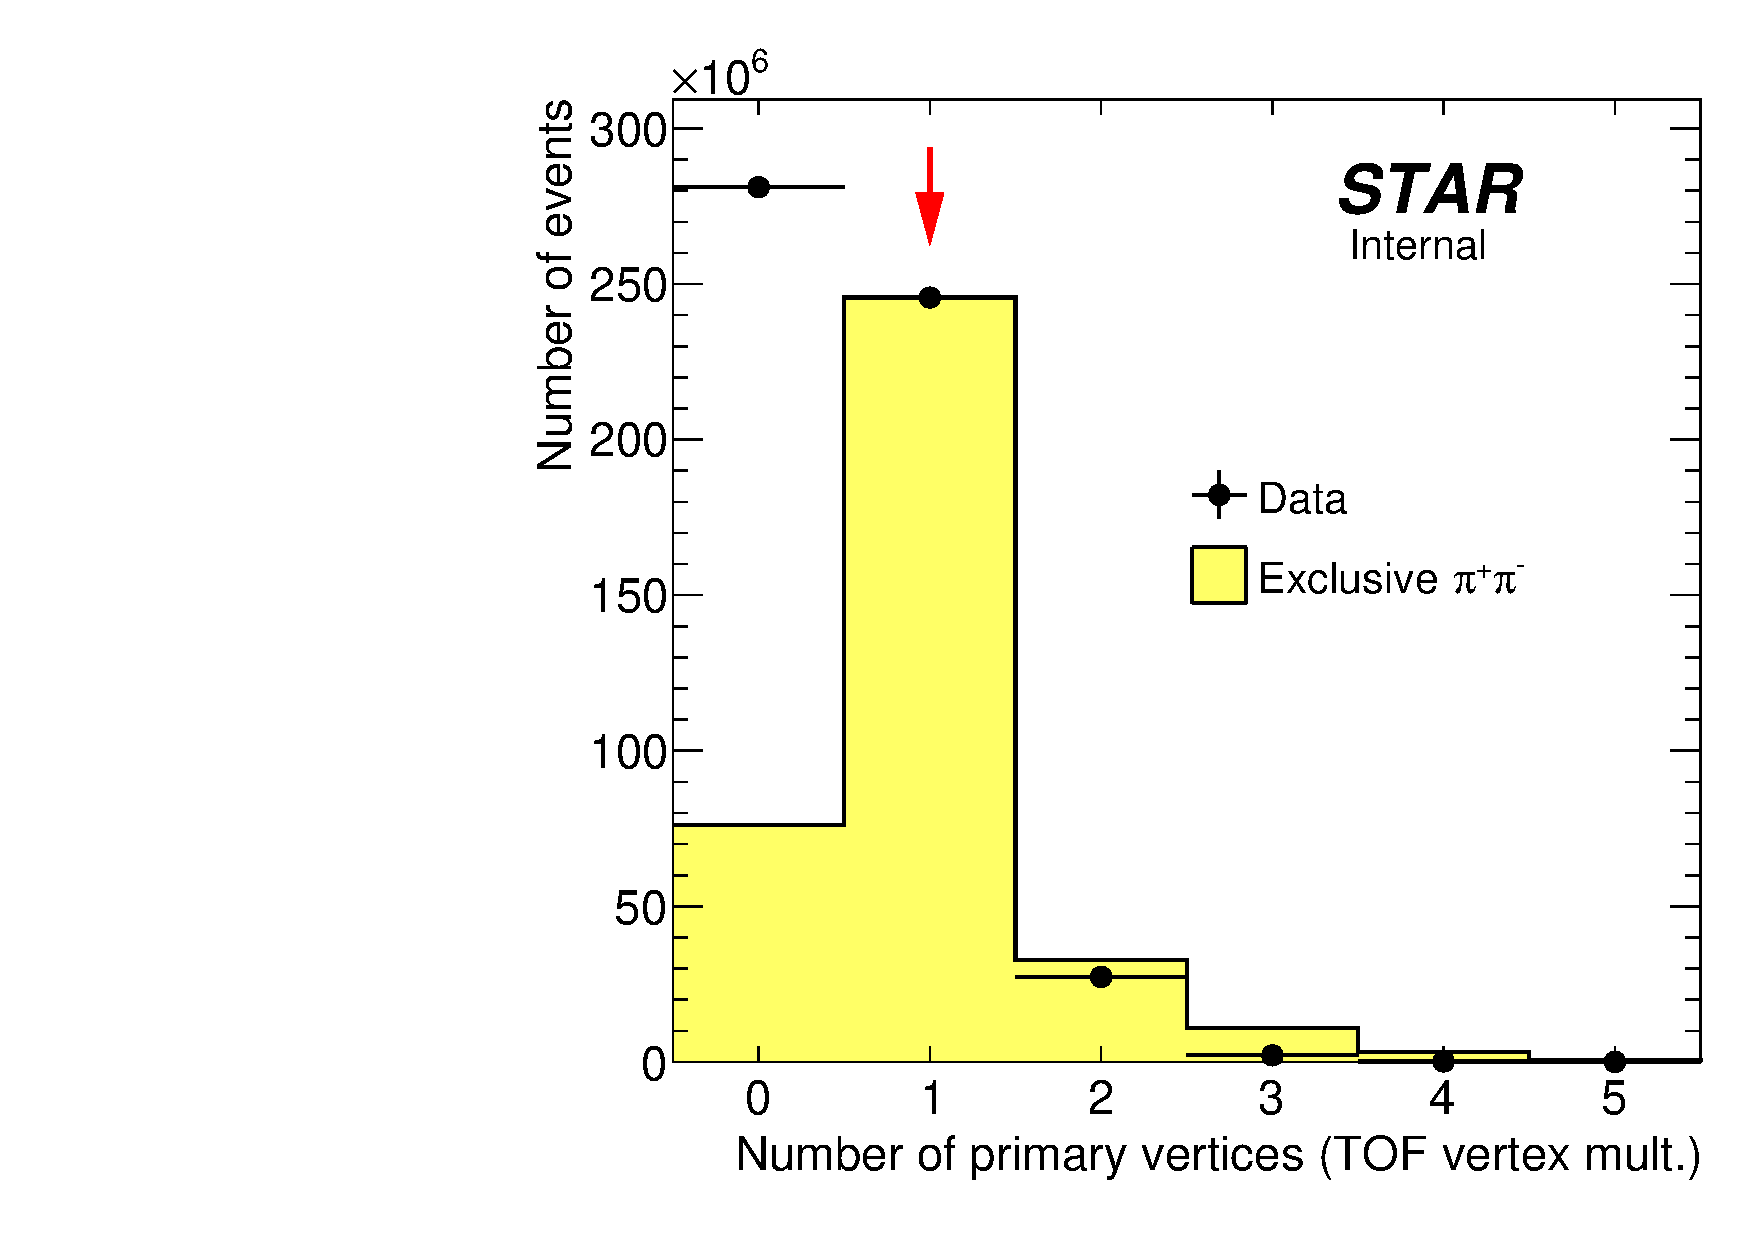
\includegraphics[width=\linewidth]{graphics/eventSelection/NumberOfPrimaryVertices.pdf}%
  \caption{Primary vertex multiplicty. Red arrow marks bin with events with exactly one primary vertex (with track(s) matched with hit in TOF), which are used in physics analysis.}\label{fig:NumberOfPrimaryVertices}
\end{minipage}%
\quad\quad%
\begin{minipage}{.4725\textwidth}%
  \centering
  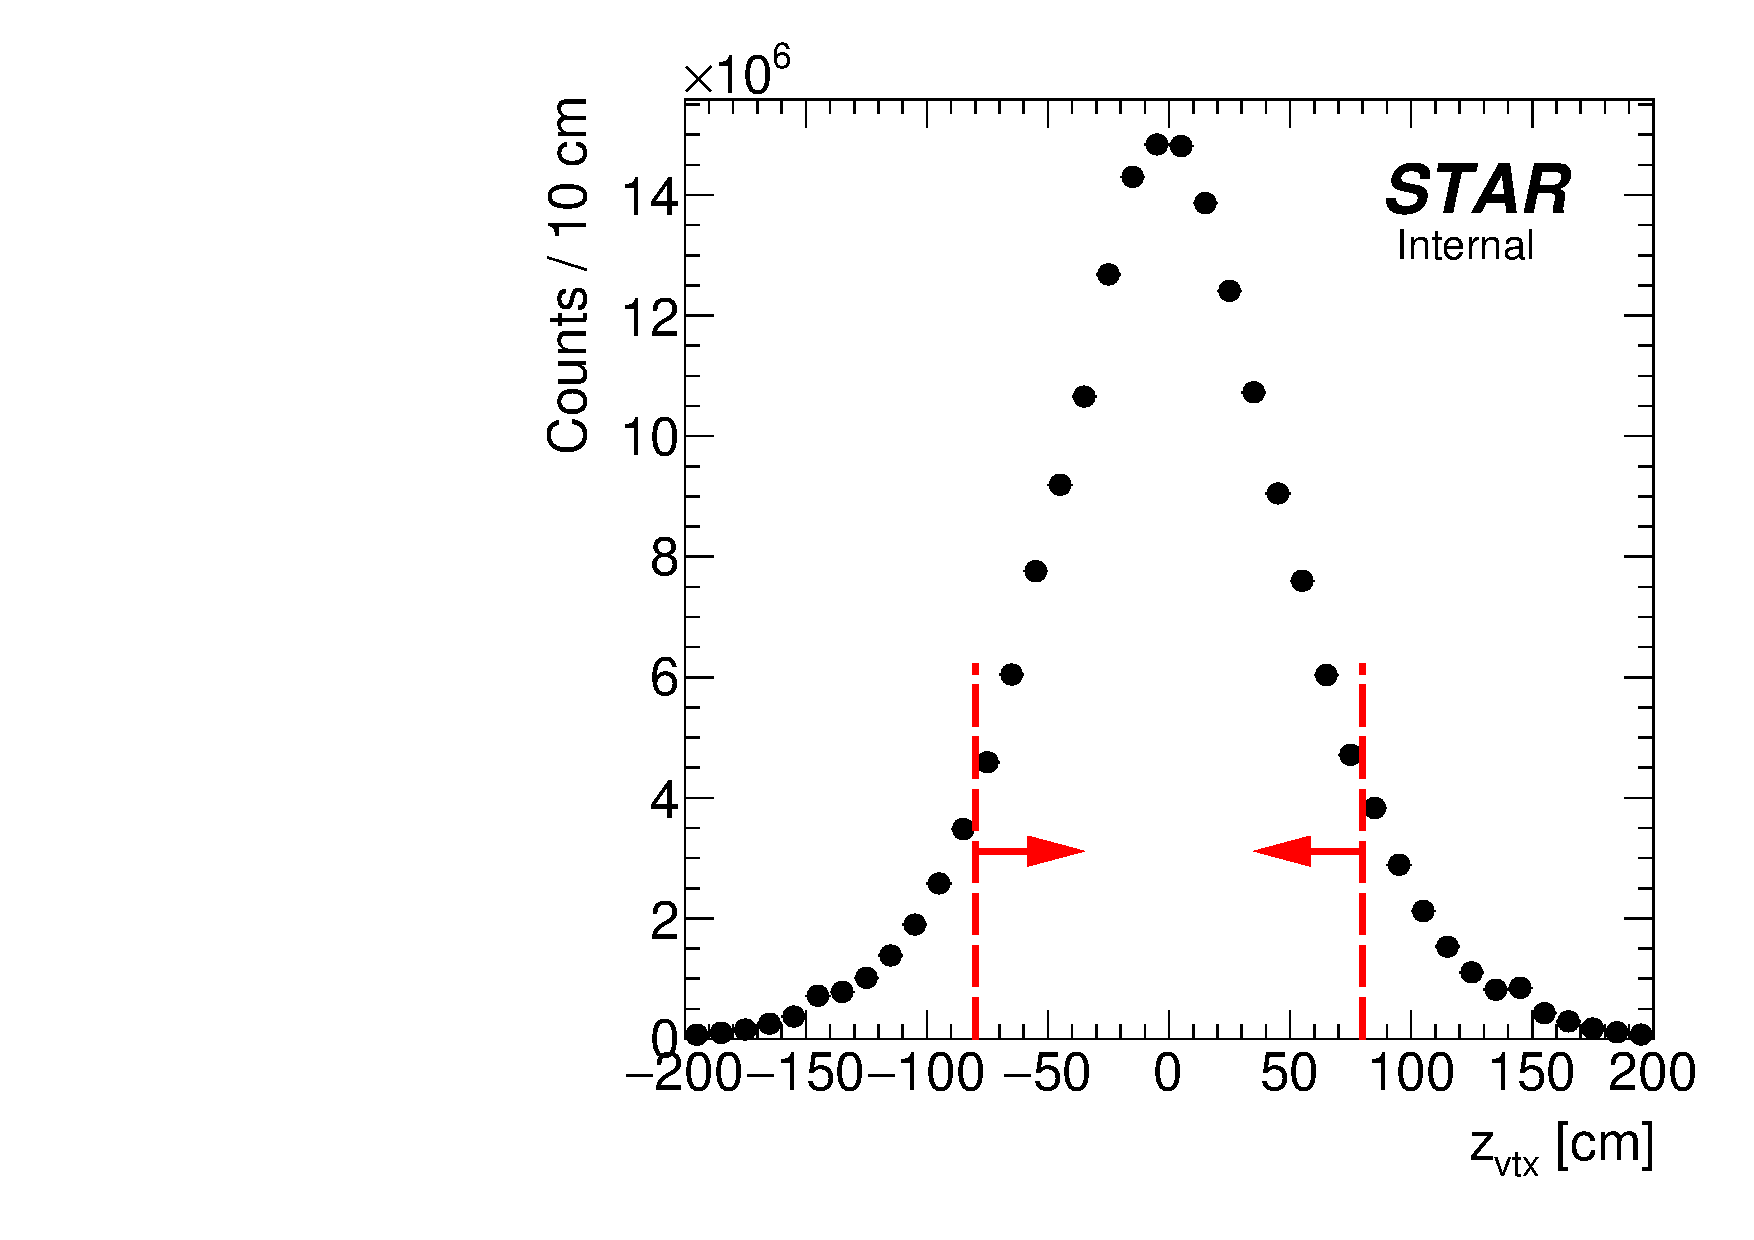
\includegraphics[width=\linewidth]{graphics/eventSelection/zVertex_oneTof.pdf}%
  \caption{\texorpdfstring{$z$}{z}-position of the primary vertex in single TOF vertex events. Red dashed line indicate range of longitudinal vertex position accepted in analysis.\newline}\label{fig:zVertexTpc}
\end{minipage}%
\end{figure}%
%---------------------------


The single TOF vertex is required to be placed within a range $(-80~\text{cm},~80~\text{cm})$ along the $z$-axis~(Fig.~\ref{fig:zVertexTpc}). Events with vertices away from the nominal IP have low acceptance both for the central tracks and the forward protons (comparing to events with vertices close to nominal IP), therefore we reject them as their inclusion to analysis would naturally introduce large systematic uncertainties. See Sec.~3.2.3 in Ref.~\cite{supplementaryNote}



















\subsection{(\ref{enum:CutTpcTrks})~TPC tracks}

The TPC track selection starts from the selection of events with exactly two primary tracks matched with hit in TOF~(Fig.~\ref{fig:NumberOfTofTracksInSingleTofVertex}). Matching with TOF guarantee that analyzed tracks originate from the triggered bunch crossing (ensures that tracks are ''in-time``). It is in accordance with the trigger logic which required at least 2 L0 TOF hits, as well as it enables more accurate particle identification with merged time-of-flight and $dE/dx$ method, comparing to sole usage of $dE/dx$. Primary tracks not matched with hit in TOF, whose average multiplicty in single TOF vertex is $\sim$8, are hardly distinguished between real and fake (off-time) tracks, which is an additional reason for not analyzing events with only one TOF-matched primary TPC track (the other track might be unmatched due to TOF inefficiency).

%---------------------------
\begin{figure}[t!]%
\centering%
\begin{minipage}{.4725\textwidth}%
  \centering%
  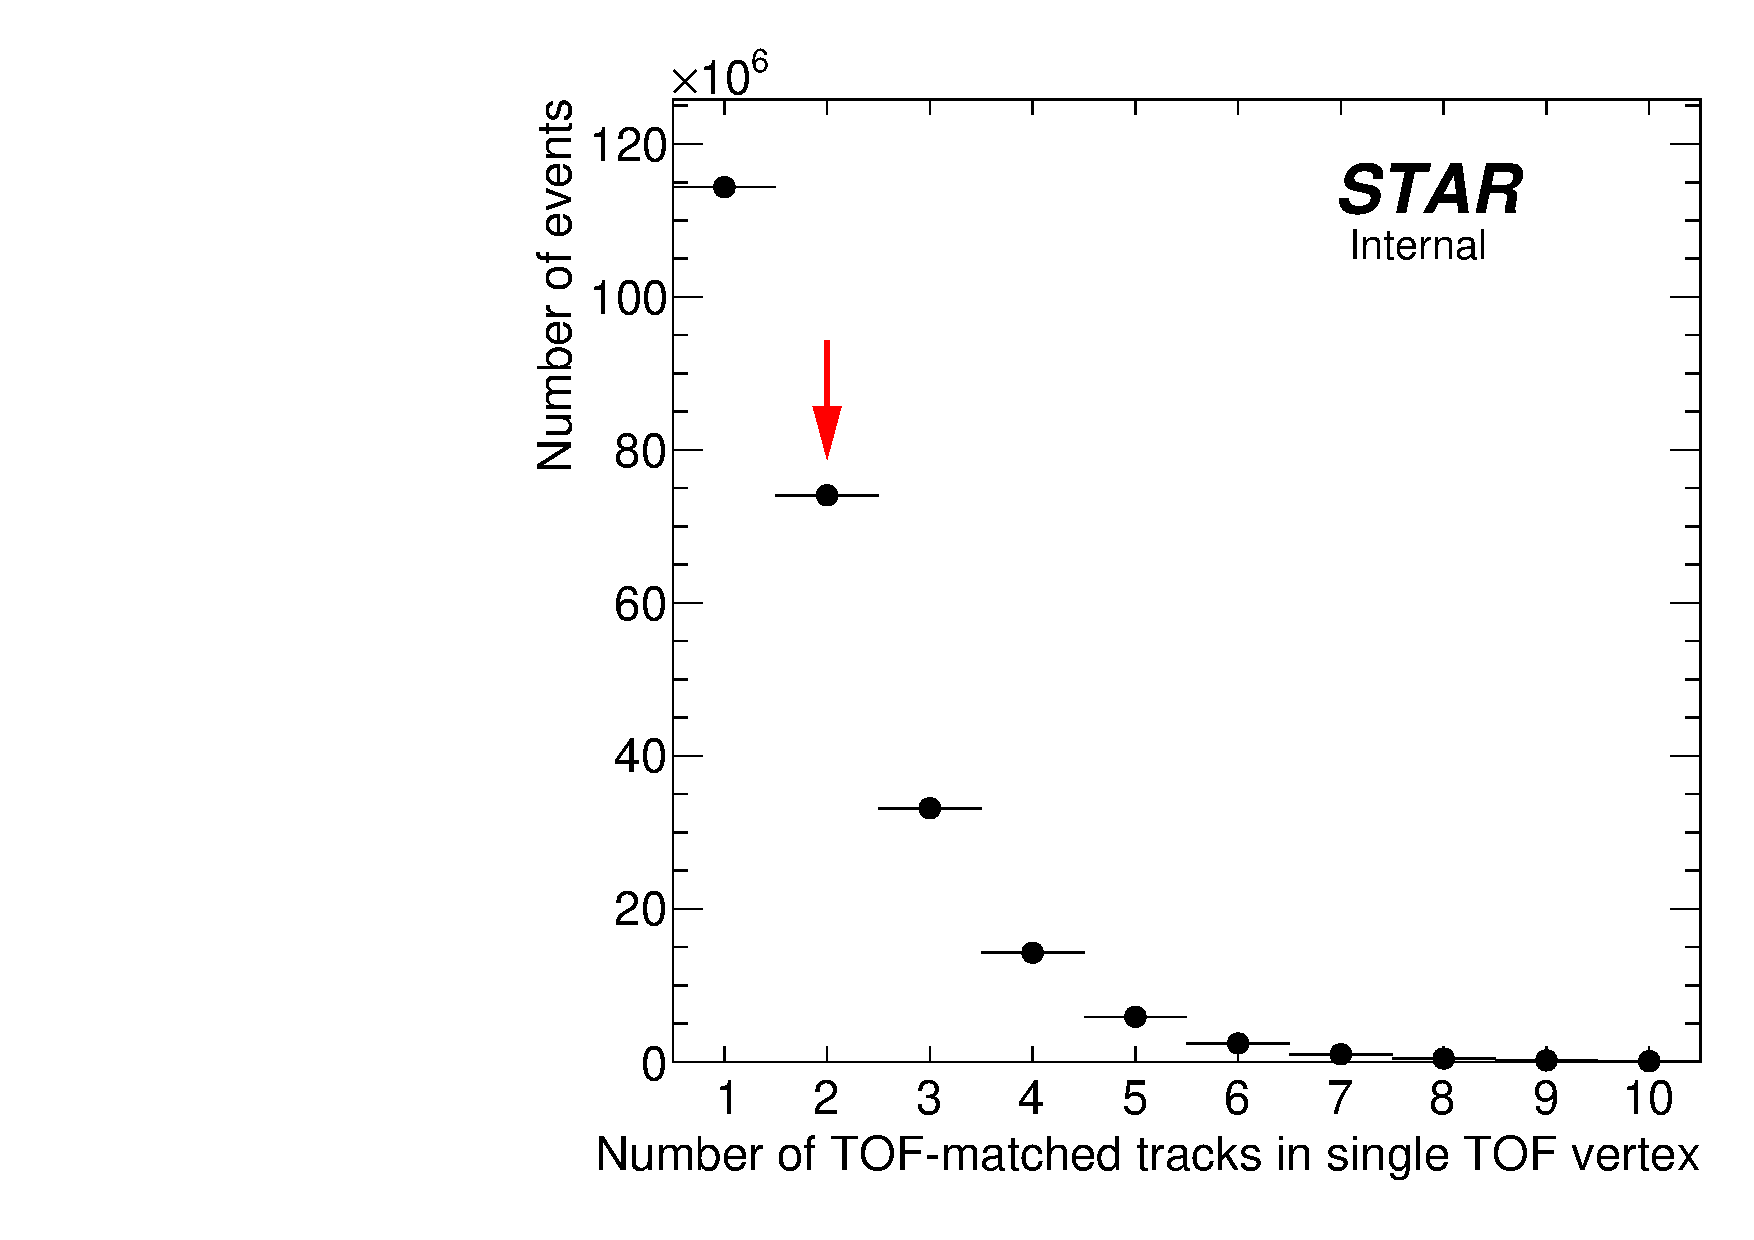
\includegraphics[width=\linewidth]{graphics/eventSelection/TpcTracks/NumberOfTofTracksInSingleTofVertex.pdf}%
  \caption[Multiplicty of primary TPC tracks matched with hit in TOF for single TOF vertex events]{Multiplicty of primary TPC tracks matched with hit in TOF for single TOF vertex events. Red arrow marks bin with events with exactly two primary tracks matched with hit in TOF, which are used in physics analysis.\newline}\label{fig:NumberOfTofTracksInSingleTofVertex}
\end{minipage}%
\quad\quad%
\begin{minipage}{.4725\textwidth}%
  \centering
  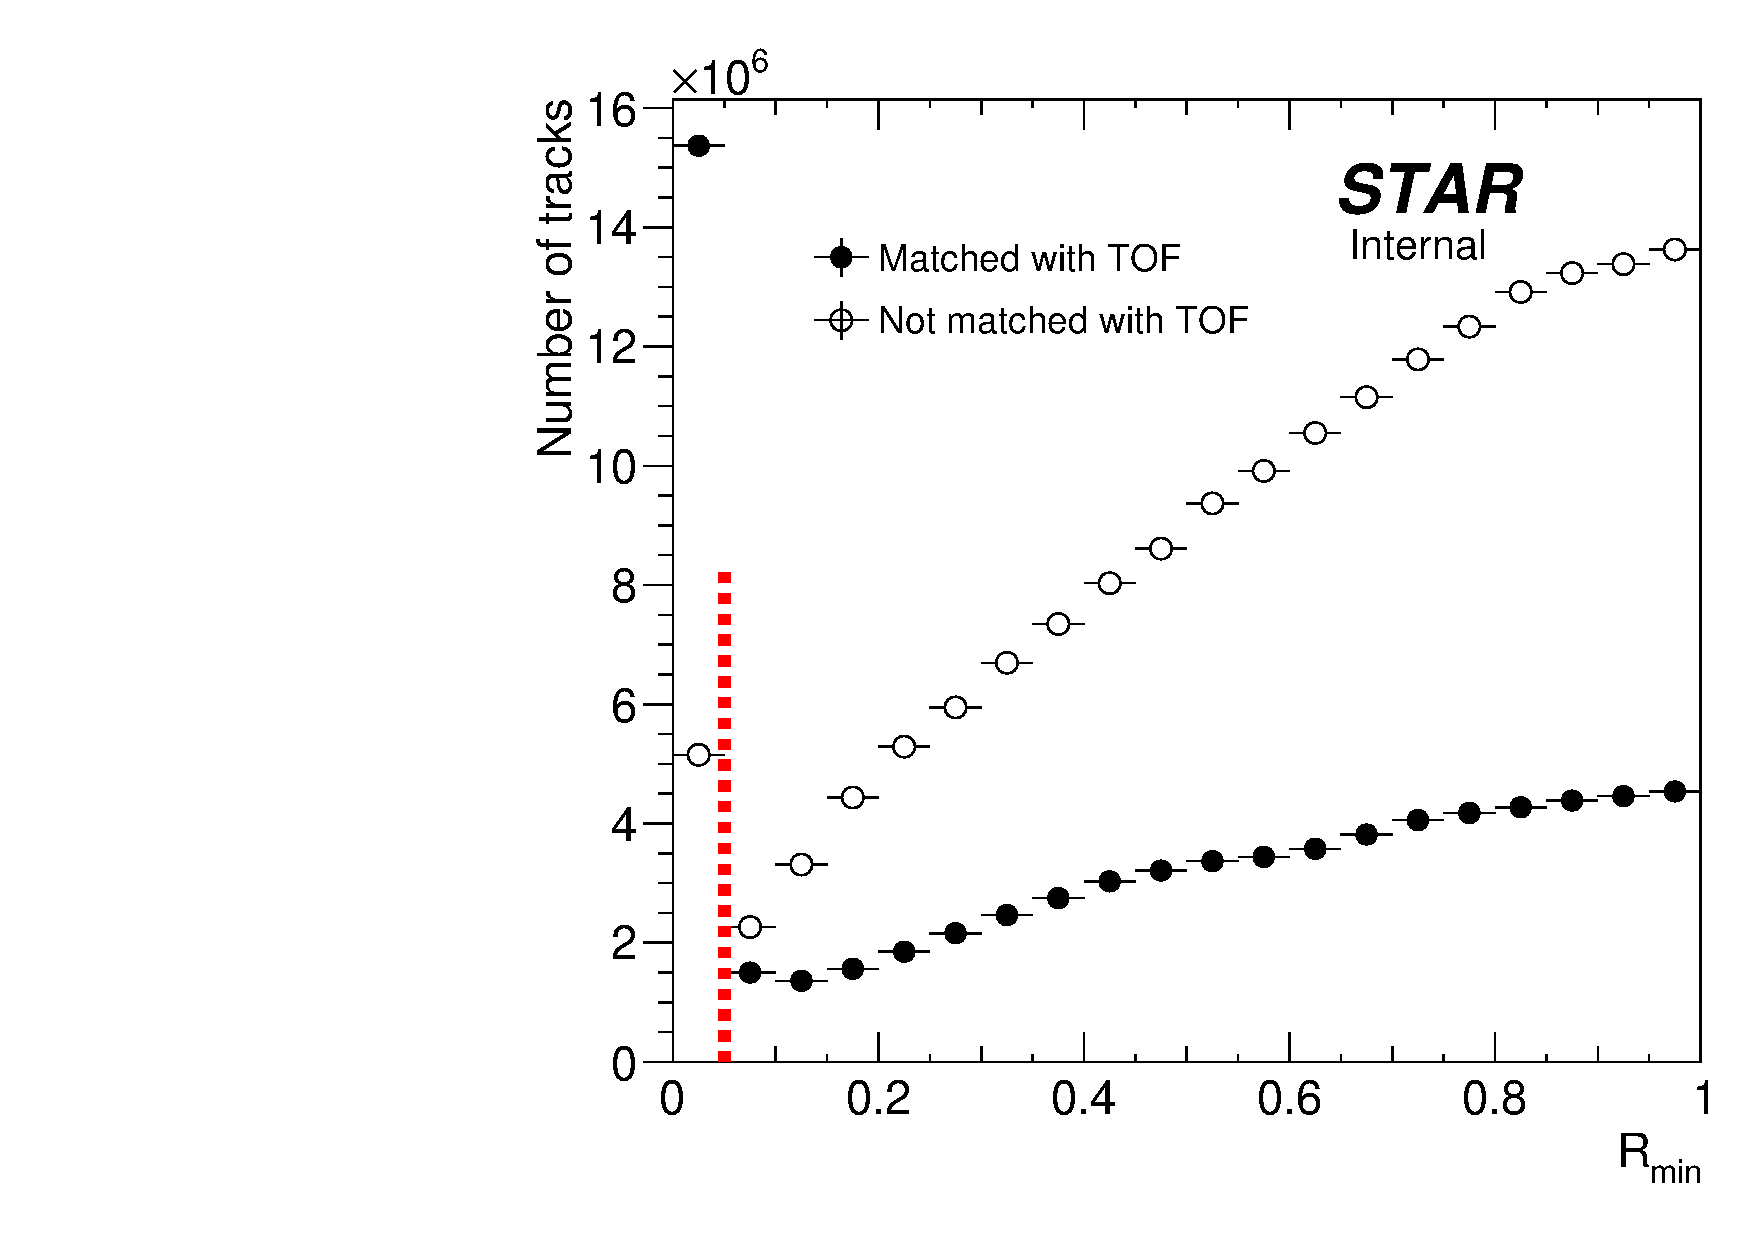
\includegraphics[width=\linewidth]{graphics/eventSelection/TpcTracks/Rmin.pdf}%
  \caption[Distribution of a distance in $\eta-\phi$ space between the BEMC cluster closest to primary TPC track ($R_{\text{min}}$)]{Distribution of a distance in $\eta-\phi$ space between the BEMC cluster closest to primary TPC track matched (filled circle) or not matched (opened circle) with hit in TOF, for single TOF vertex events. Red dashed line indicate matching threshold $R^{\text{match}}_{\text{max}} = 0.05$.}\label{fig:Rmin} %which are expected to reack BEMC
\end{minipage}%
\end{figure}%
%---------------------------

Primary TPC tracks from the single TOF vertex which are matched with TOF are allowed to be also matched with BEMC clusters. Matching with BEMC cluster is claimed if the distance in $\eta-\phi$ space between the BEMC cluster position $(\eta_{\text{clus}},~\phi_{\text{clus}})$ and projected position of the track in BEMC $(\eta_{\text{proj}},~\phi_{\text{proj}})$, defined as
\begin{equation}
 R=\sqrt{(\eta_{\text{clus}}-\eta_{\text{proj}})^{2} + (\phi_{\text{clus}}-\phi_{\text{proj}})^{2}},
\end{equation}
is less than $R^{\text{match}}_{\text{max}} = 0.05$. Distribution of the distance between the primary TPC track and the closest BEMC cluster is shown in~Fig.~\ref{fig:Rmin}.

However, if there are any primary TPC tracks matched with BEMC cluster and not matched with TOF in the single TOF vertex with two TOF-matched tracks, an event is rejected. Such configuration implies higher-than-2 multiplicty of the real tracks in the vertex, hence an event is unlikely a Central Exclusive Production of two particles.



%---------------------------
\begin{figure}[hb]
\centering
\parbox{0.4725\textwidth}{
  \centering
  \begin{subfigure}[b]{\linewidth}
                \subcaptionbox{\label{fig:NHitsFit}}{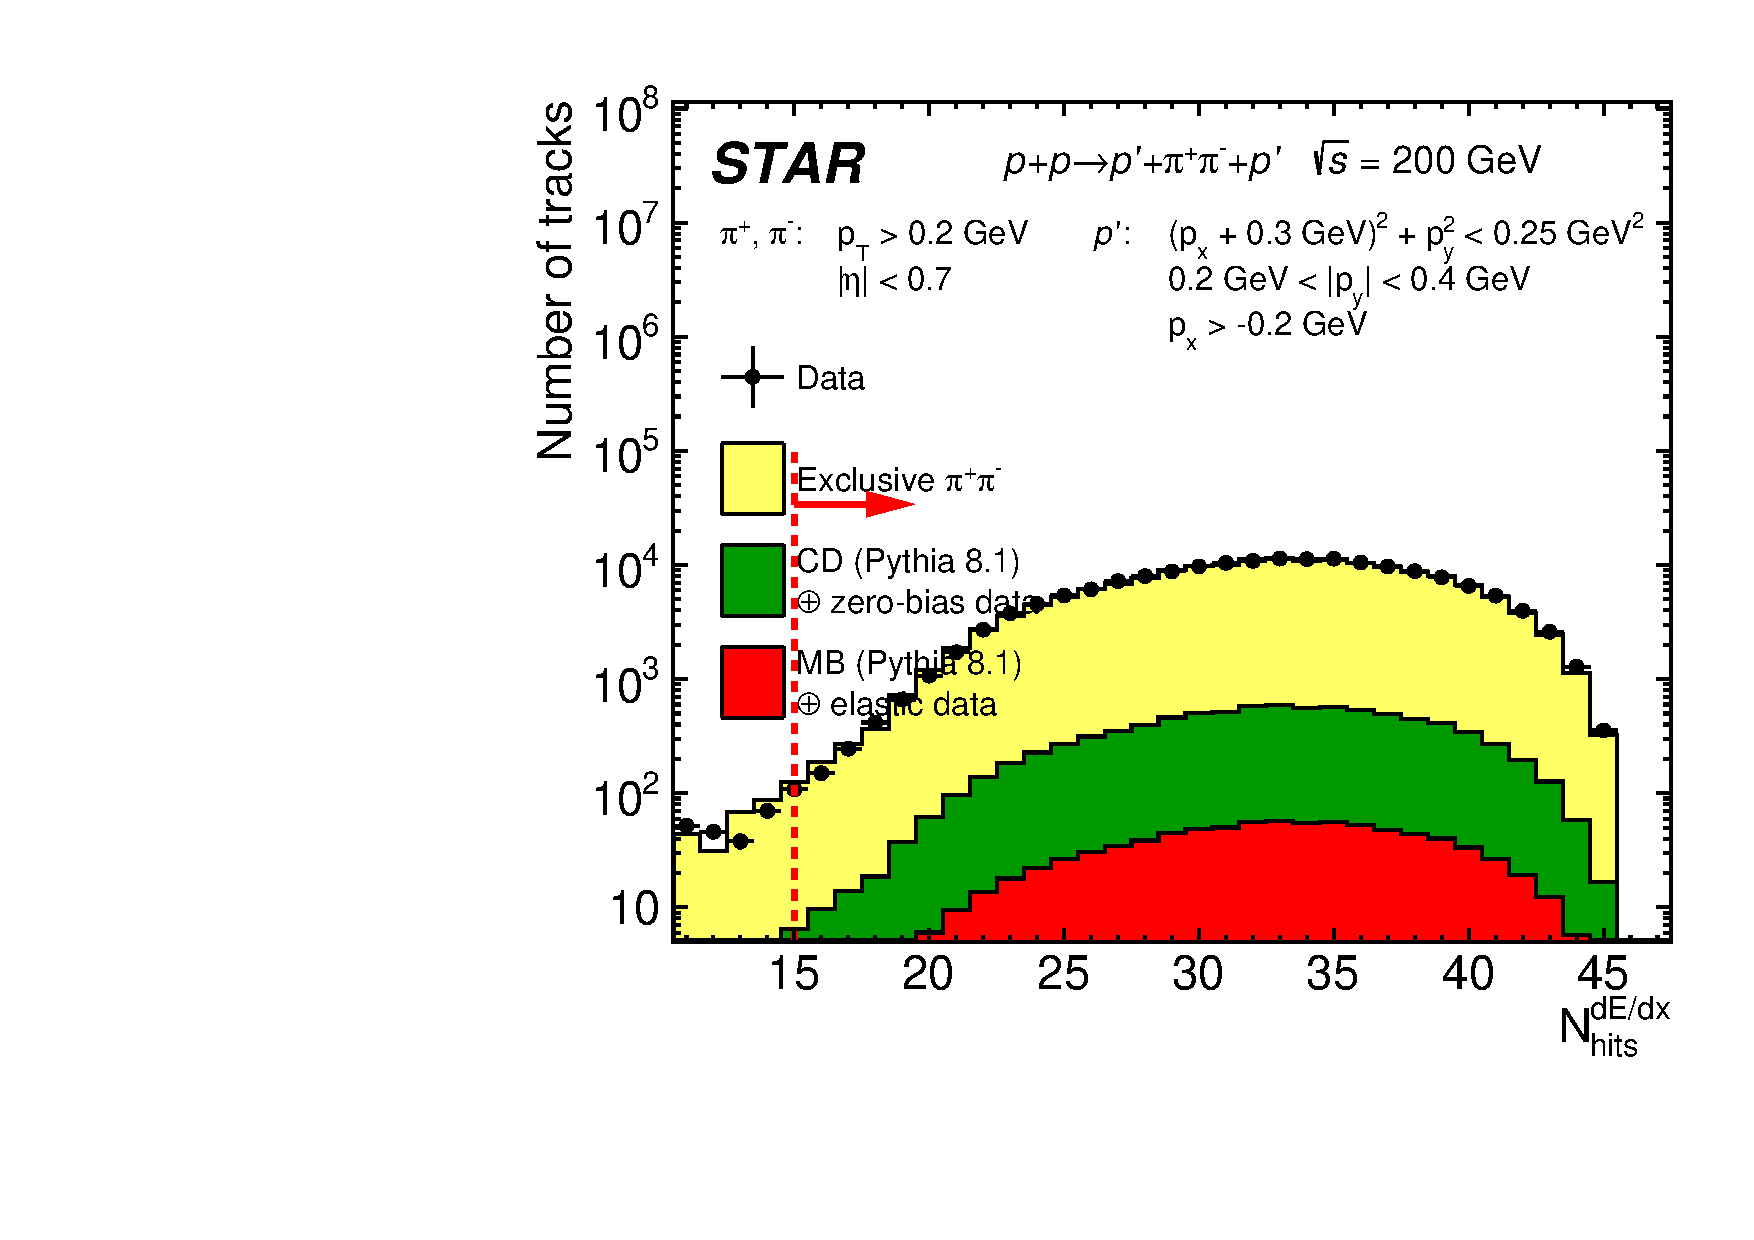
\includegraphics[width=\linewidth]{graphics/eventSelection/TpcTracks/NHitsFit.pdf}}
  \end{subfigure}\\
  \begin{subfigure}[b]{\linewidth}\addtocounter{subfigure}{1}
                \subcaptionbox{\label{fig:NHitsFit_to_NHitsPos}}{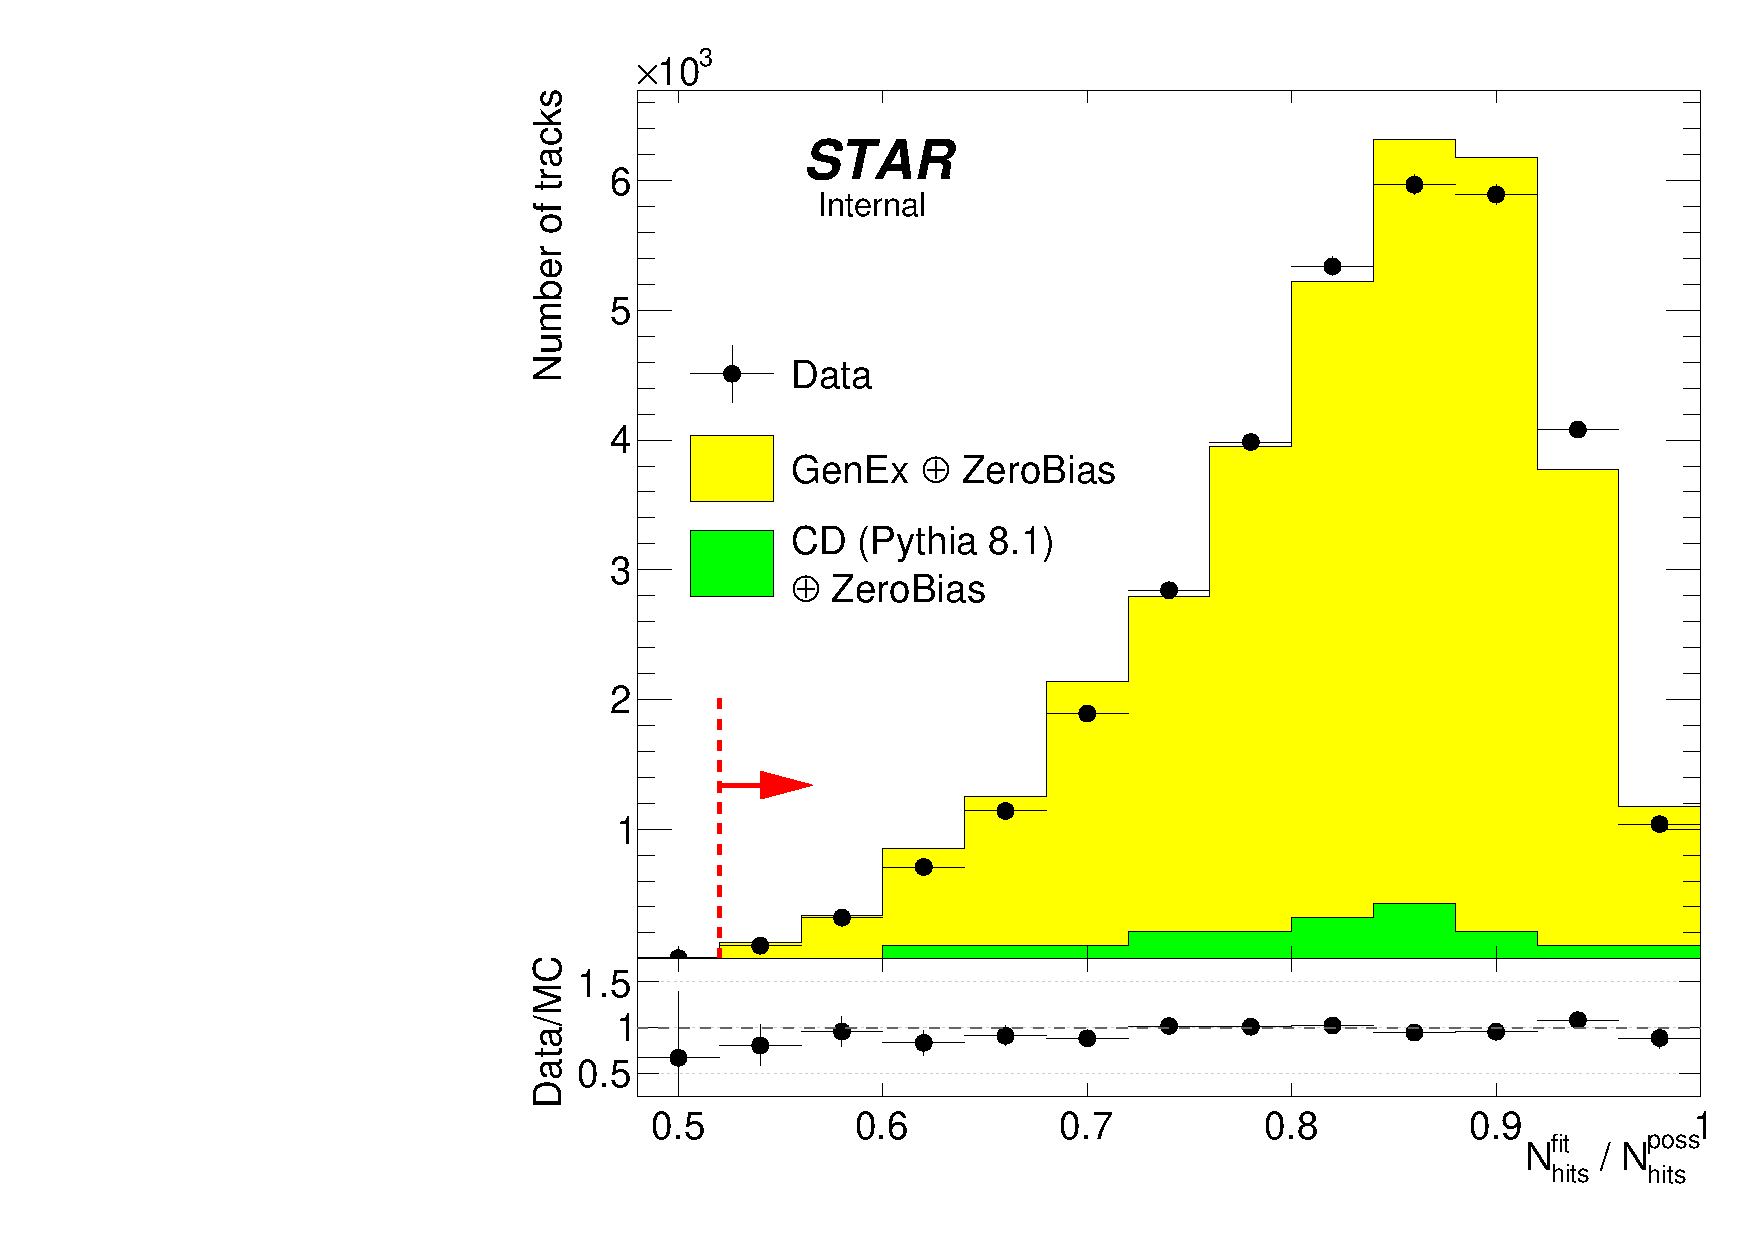
\includegraphics[width=\linewidth]{graphics/eventSelection/TpcTracks/NHitsFit_to_NHitsPos.pdf}}
  \end{subfigure}
}%
\quad\quad%
\parbox{0.4725\textwidth}{
  \centering
  \begin{subfigure}[b]{\linewidth}\addtocounter{subfigure}{-2}
                \subcaptionbox{\label{fig:NHits_dEdx}}{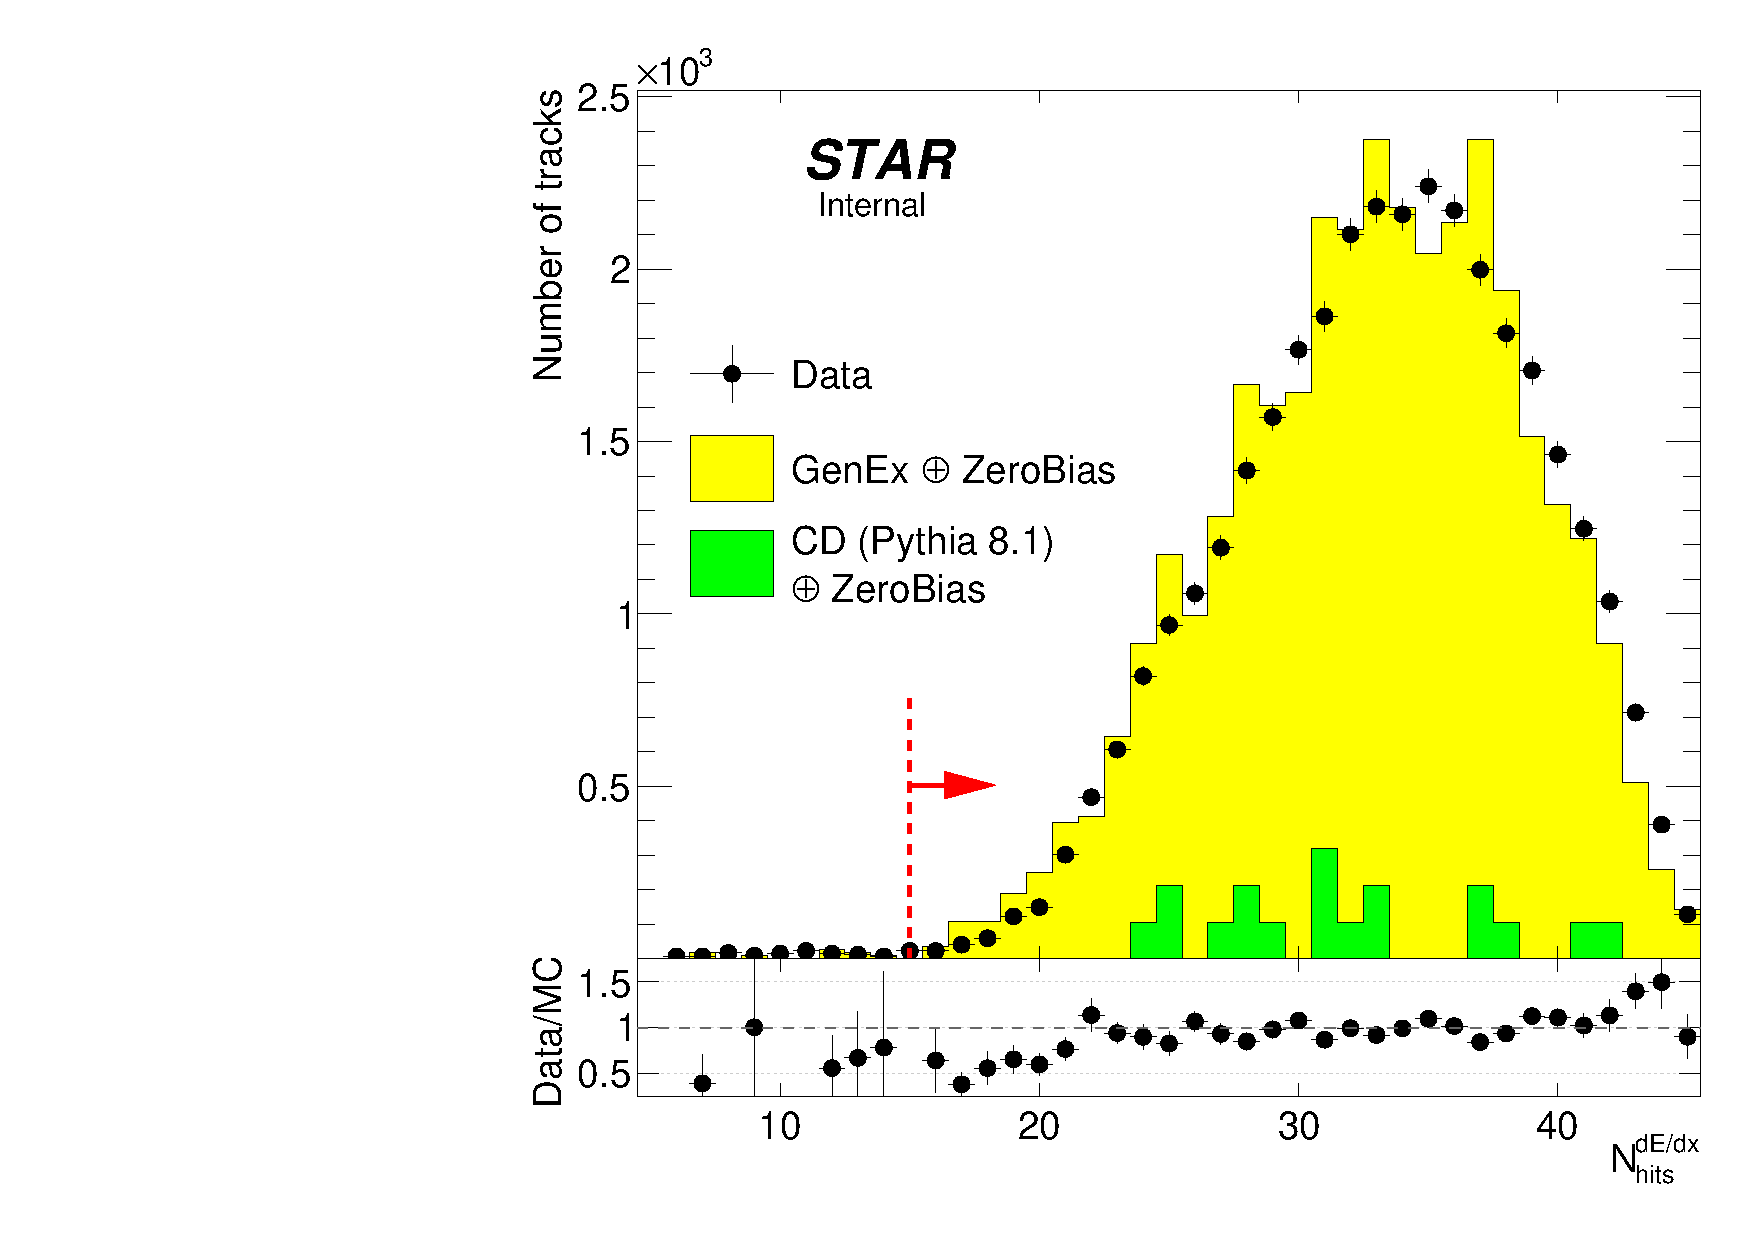
\includegraphics[width=\linewidth]{graphics/eventSelection/TpcTracks/NHits_dEdx.pdf}}
  \end{subfigure}\\
  \begin{minipage}[t][1.042\linewidth][t]{\linewidth}\vspace{10pt}
    \caption[Comparison of distribution of $N_{\text{hits}}^{\text{fit}}$,~$N_{\text{hits}}^{\text{dE/dx}}$ and $N_{\text{hits}}^{\text{fit}}/N_{\text{hits}}^{\text{poss}}$ in the data and embedded MC]
    {Comparison of distribution of the number of hits used in TPC track reconstrucion $N_{\text{hits}}^{\text{fit}}$ (\ref{fig:NHitsFit}), number of hits used in specific energy loss reconstrucion $N_{\text{hits}}^{\text{dE/dx}}$ (\ref{fig:NHits_dEdx}) and fraction of number of hits potentially generated by the track and finally used in the reconstrucion $N_{\text{hits}}^{\text{fit}}/N_{\text{hits}}^{\text{poss}}$ (\ref{fig:NHitsFit_to_NHitsPos}) in the data and embedded MC. Normalizations of the signal and backgrounds were established from the comparison of $p_{T}^{\text{miss}}$ and $\Delta\theta$ distributions after full selection (without cut on the presented quantity and without exclusivity cut), as described in Sec.~\ref{sec:bkgdSignalNorm}. Red dashed line and red arrow indicate the range of each quantity which is accepted in analysis.}\label{fig:NHits}
  \end{minipage}
}%

\end{figure}
%---------------------------







% %---------------------------
% \begin{figure}[ht!]
% \centering
% \parbox{0.4725\textwidth}{
%   \centering
%   \begin{subfigure}[b]{\linewidth}{
%                 \subcaptionbox{\label{fig:d0}}{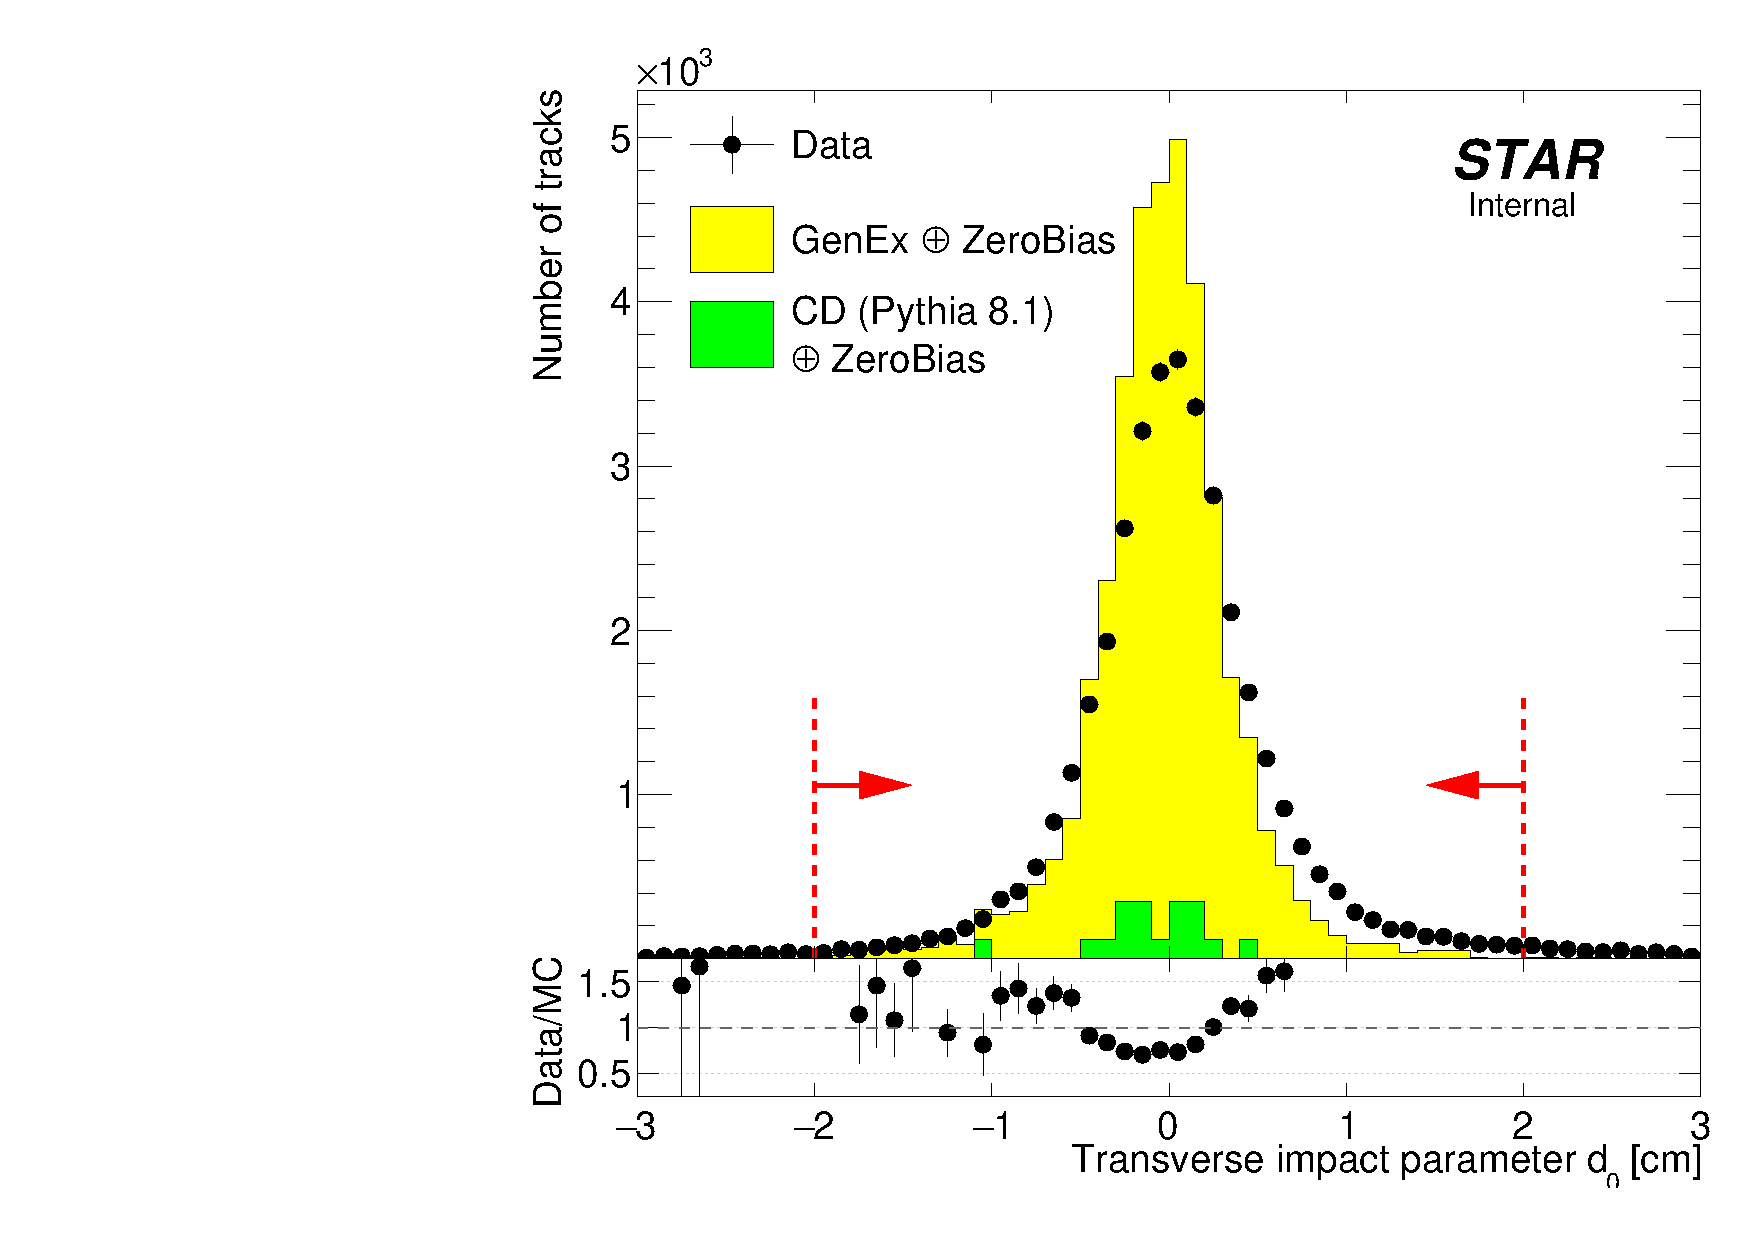
\includegraphics[width=\linewidth]{graphics/eventSelection/TpcTracks/d0.pdf}}}
%   \end{subfigure}
% }%
% \quad\quad%
% \parbox{0.4725\textwidth}{%
%   \centering
%   \begin{subfigure}[b]{\linewidth}{
%                 \subcaptionbox{\label{fig:z0}}{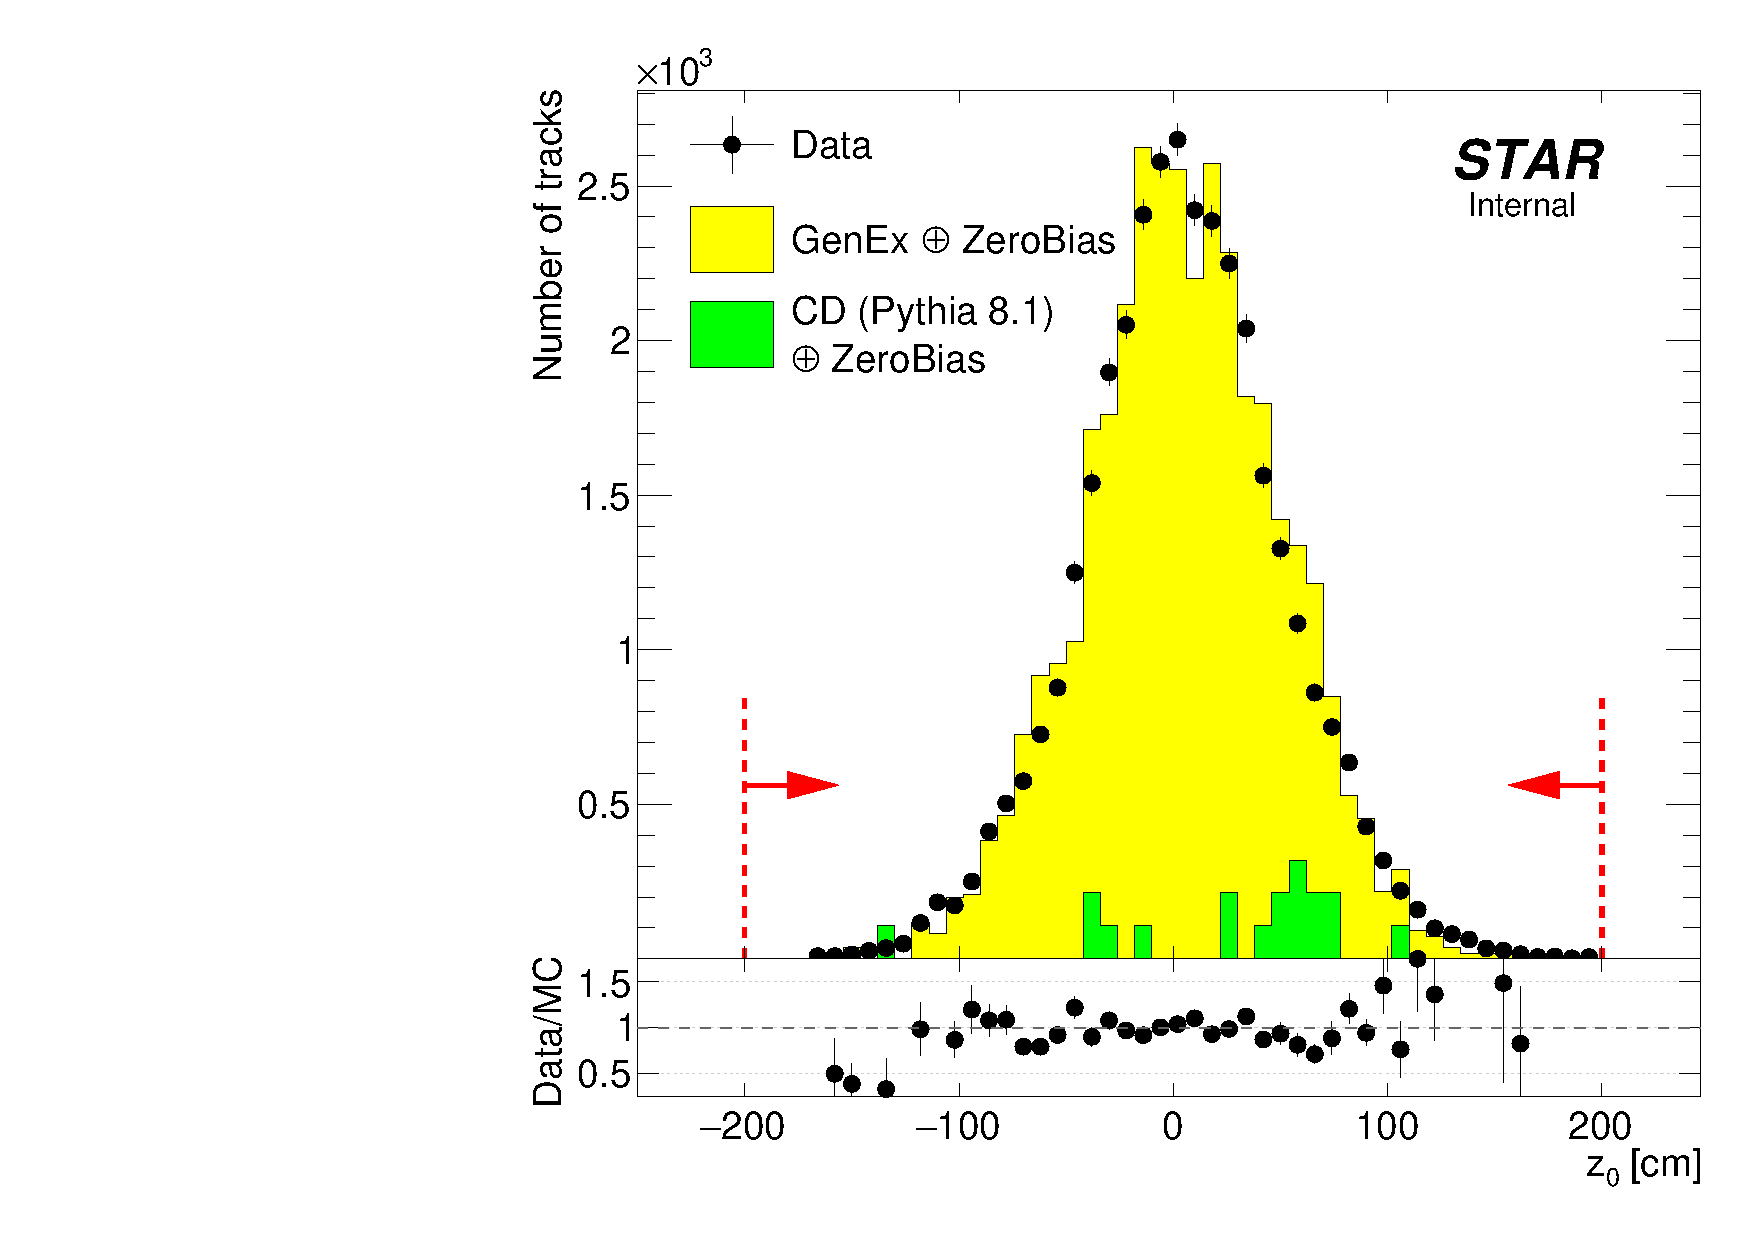
\includegraphics[width=\linewidth]{graphics/eventSelection/TpcTracks/z0.pdf}}}
%   \end{subfigure}
% }%
% \caption[Comparison of distribution of $d_{0}$ and $z_{0}$ in the data and embedded MC]
% {Comparison of distribution of the transverse impact parameter $d_{0}$ (\ref{fig:d0}) and the longitudinal impact parameter $z_{0}$ (\ref{fig:z0}) in the data and embedded MC. Normalizations of the signal and backgrounds were established from the comparison of $p_{T}^{\text{miss}}$ and $\Delta\theta$ distributions after full selection (without cut on the presented quantity and without exclusivity cut), as described in Sec.~\ref{sec:bkgdSignalNorm}. Red dashed lines and red arrows indicate the range of each quantity which is accepted in analysis.}\label{fig:d0z0}
% \end{figure}
% %---------------------------





% 
% %---------------------------
% \begin{figure}[ht!]
% \centering
% \parbox{0.4725\textwidth}{
%   \centering
%   \begin{subfigure}[b]{\linewidth}{
%                 \subcaptionbox{\label{fig:RadialDca}}{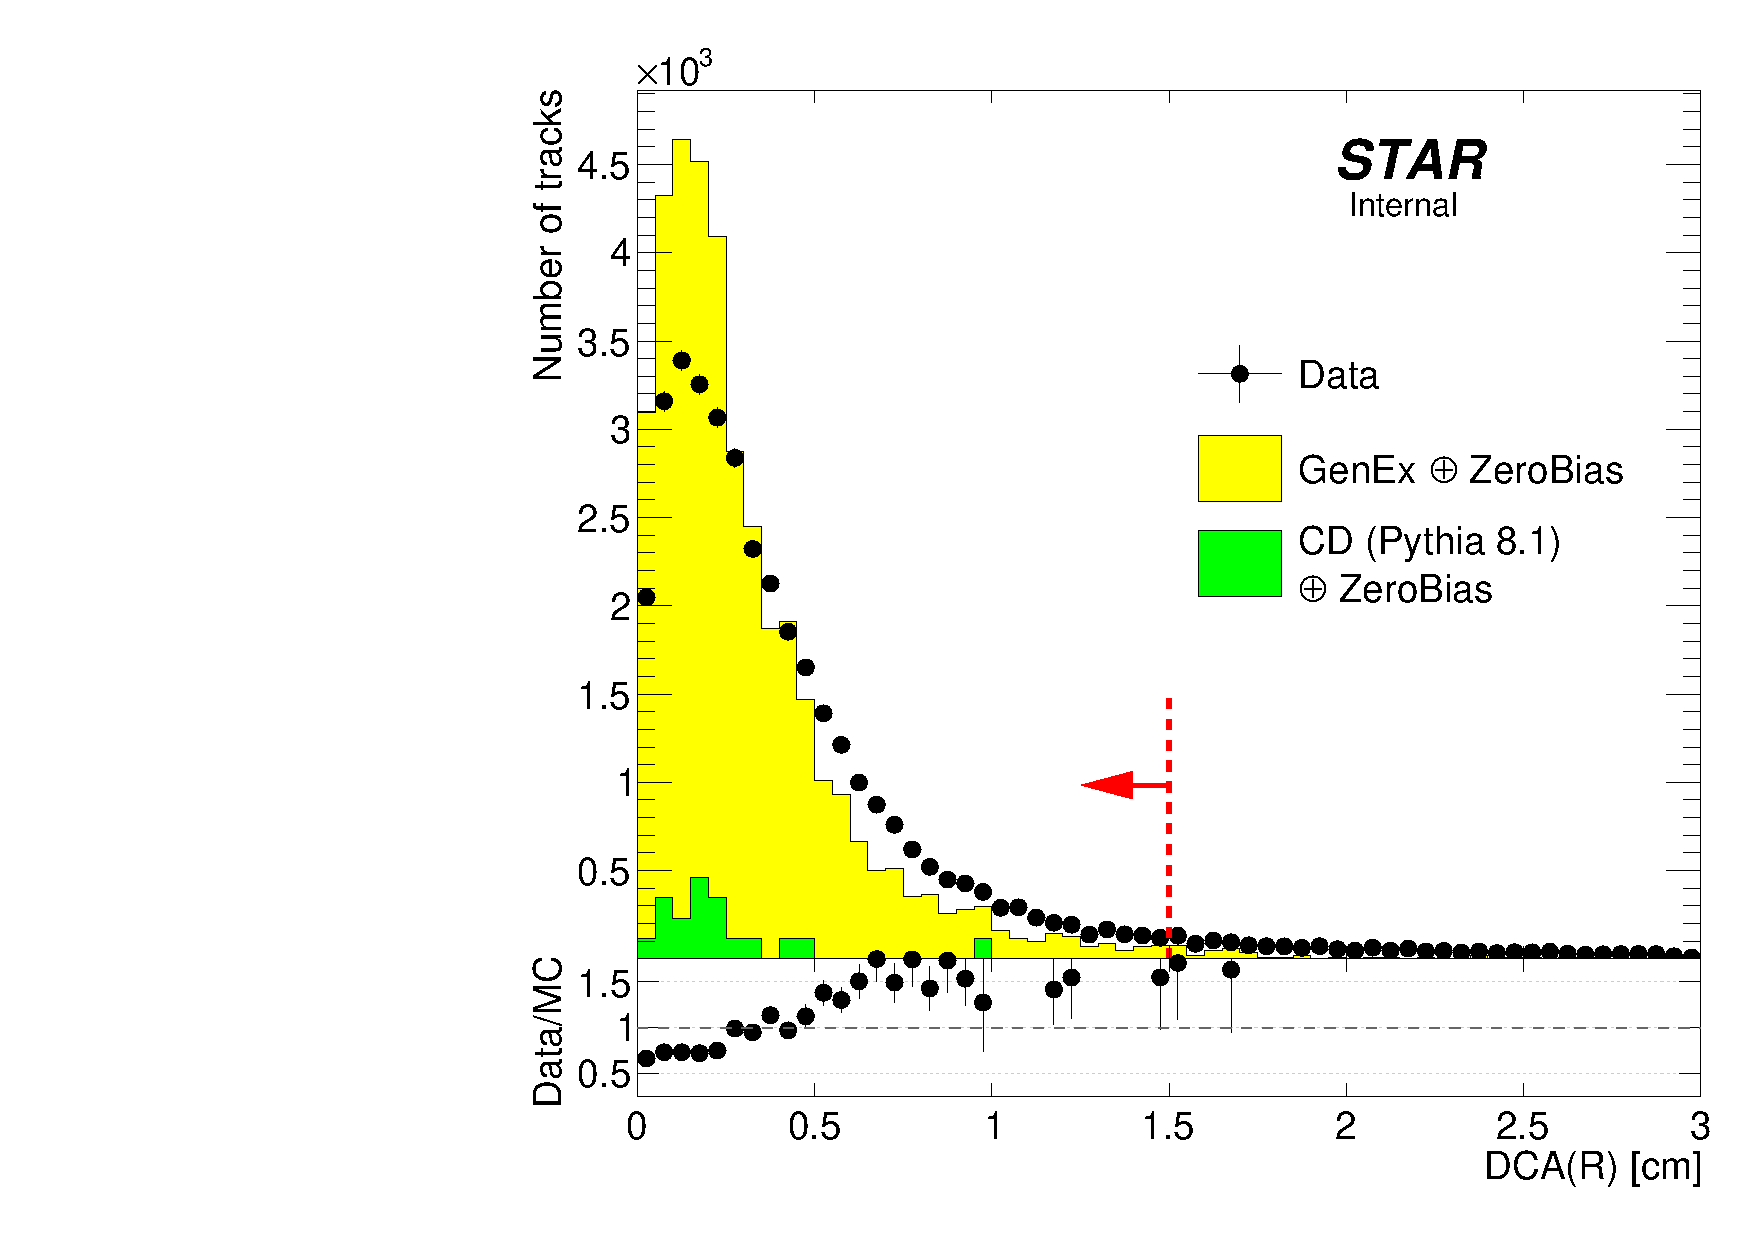
\includegraphics[width=\linewidth]{graphics/eventSelection/TpcTracks/RadialDCA.pdf}}}
%   \end{subfigure}
% }%
% \quad\quad%
% \parbox{0.4725\textwidth}{%
%   \centering
%   \begin{subfigure}[b]{\linewidth}{
%                 \subcaptionbox{\label{fig:LongitudinalDca}}{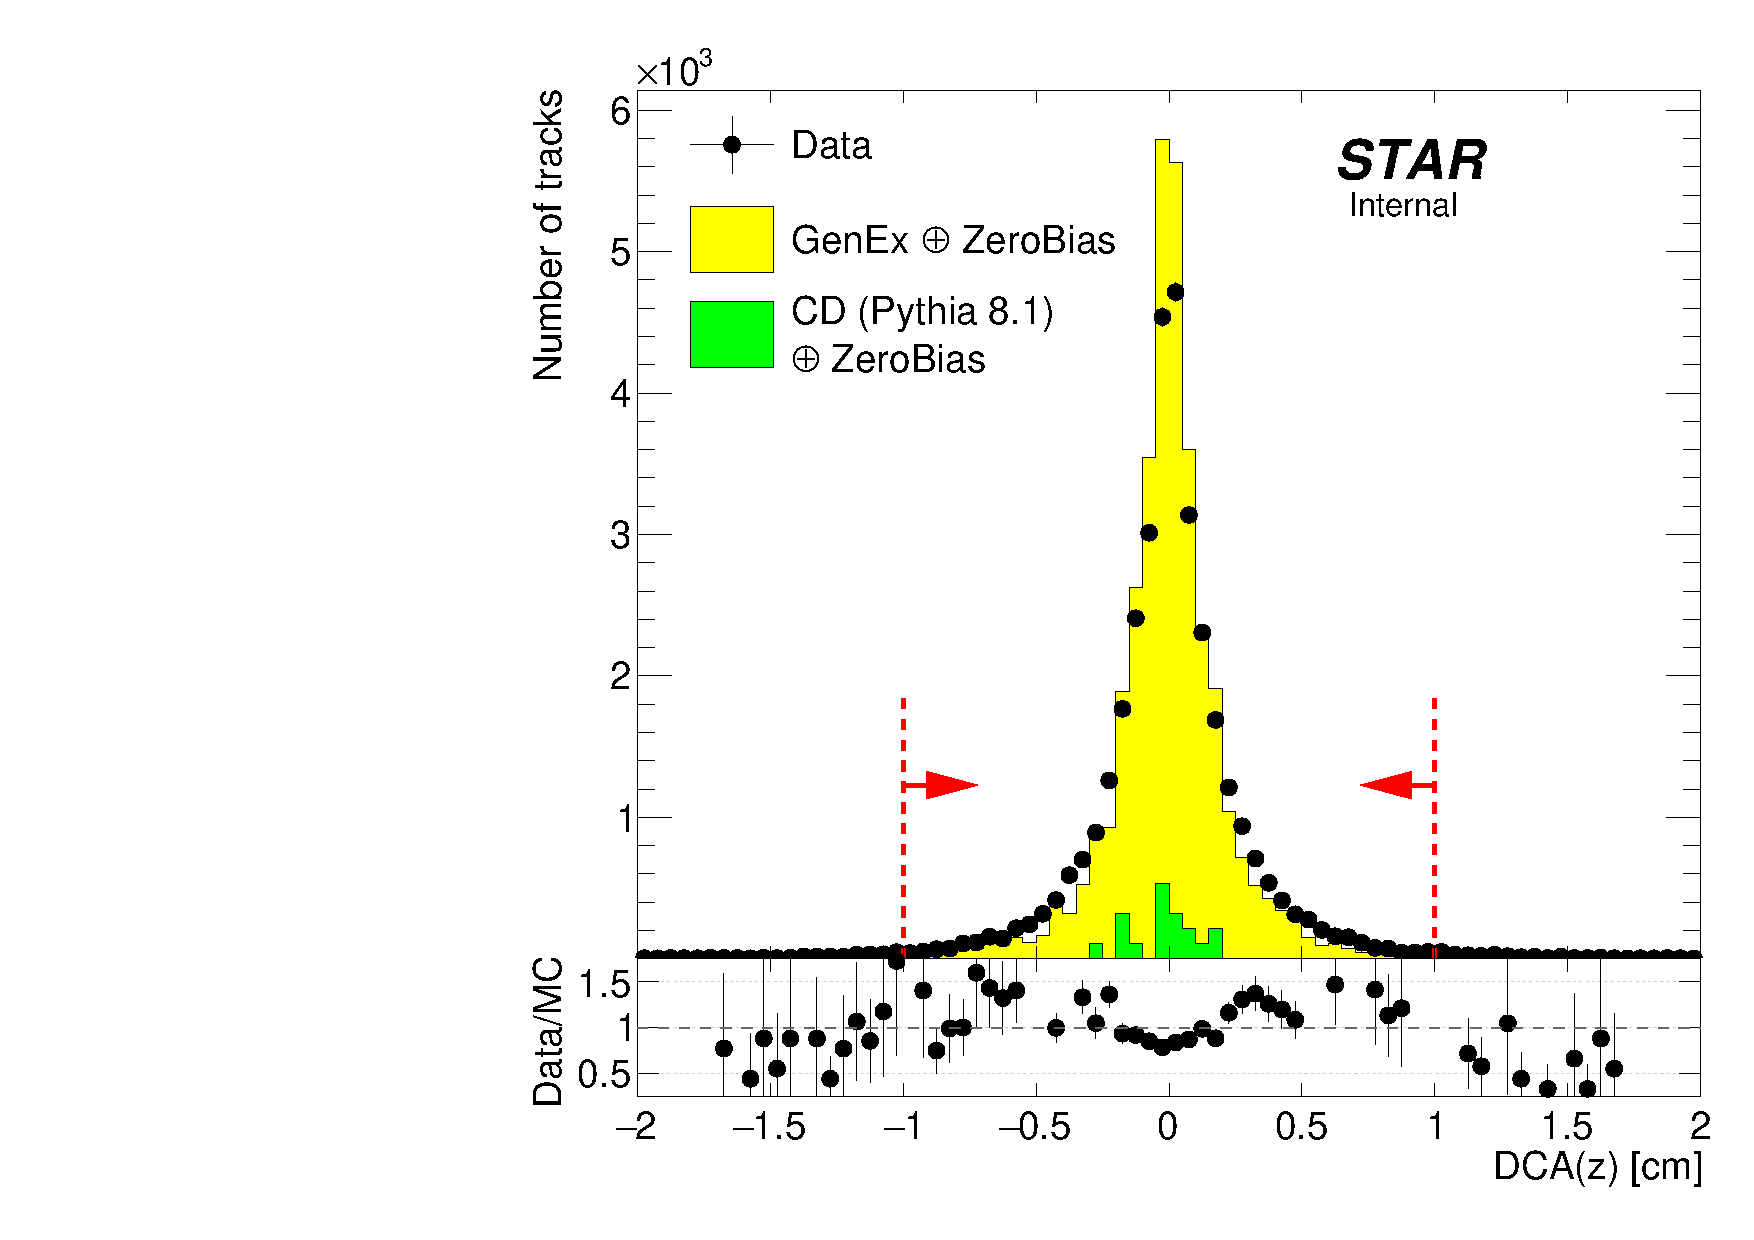
\includegraphics[width=\linewidth]{graphics/eventSelection/TpcTracks/LongitudinalDCA.pdf}}}
%   \end{subfigure}
% }%
% \caption[Comparison of distribution of $\text{DCA}(R)$ and $\text{DCA}(z)$ in the data and embedded MC]
% {Comparison of distribution of the distance of closest approach of the track to the vertex in the $xy$-plane $\text{DCA}(R)$ (\ref{fig:RadialDca}) and the the distance of closest approach of the track to the vertex along the $z$-axis $\text{DCA}(z)$ (\ref{fig:LongitudinalDca}) in the data and embedded MC. Normalizations of the signal and backgrounds were established from the comparison of $p_{T}^{\text{miss}}$ and $\Delta\theta$ distributions after full selection (without cut on the presented quantity and without exclusivity cut), as described in Sec.~\ref{sec:bkgdSignalNorm}. Red dashed lines and red arrows indicate the range of each quantity which is accepted in analysis.}\label{fig:DCA}
% \end{figure}
% %---------------------------



%---------------------------
\begin{figure}[ht!]
\centering
\parbox{0.4725\textwidth}{
  \centering
  \begin{subfigure}[b]{\linewidth}{
                \subcaptionbox{\label{fig:TrackEta}}{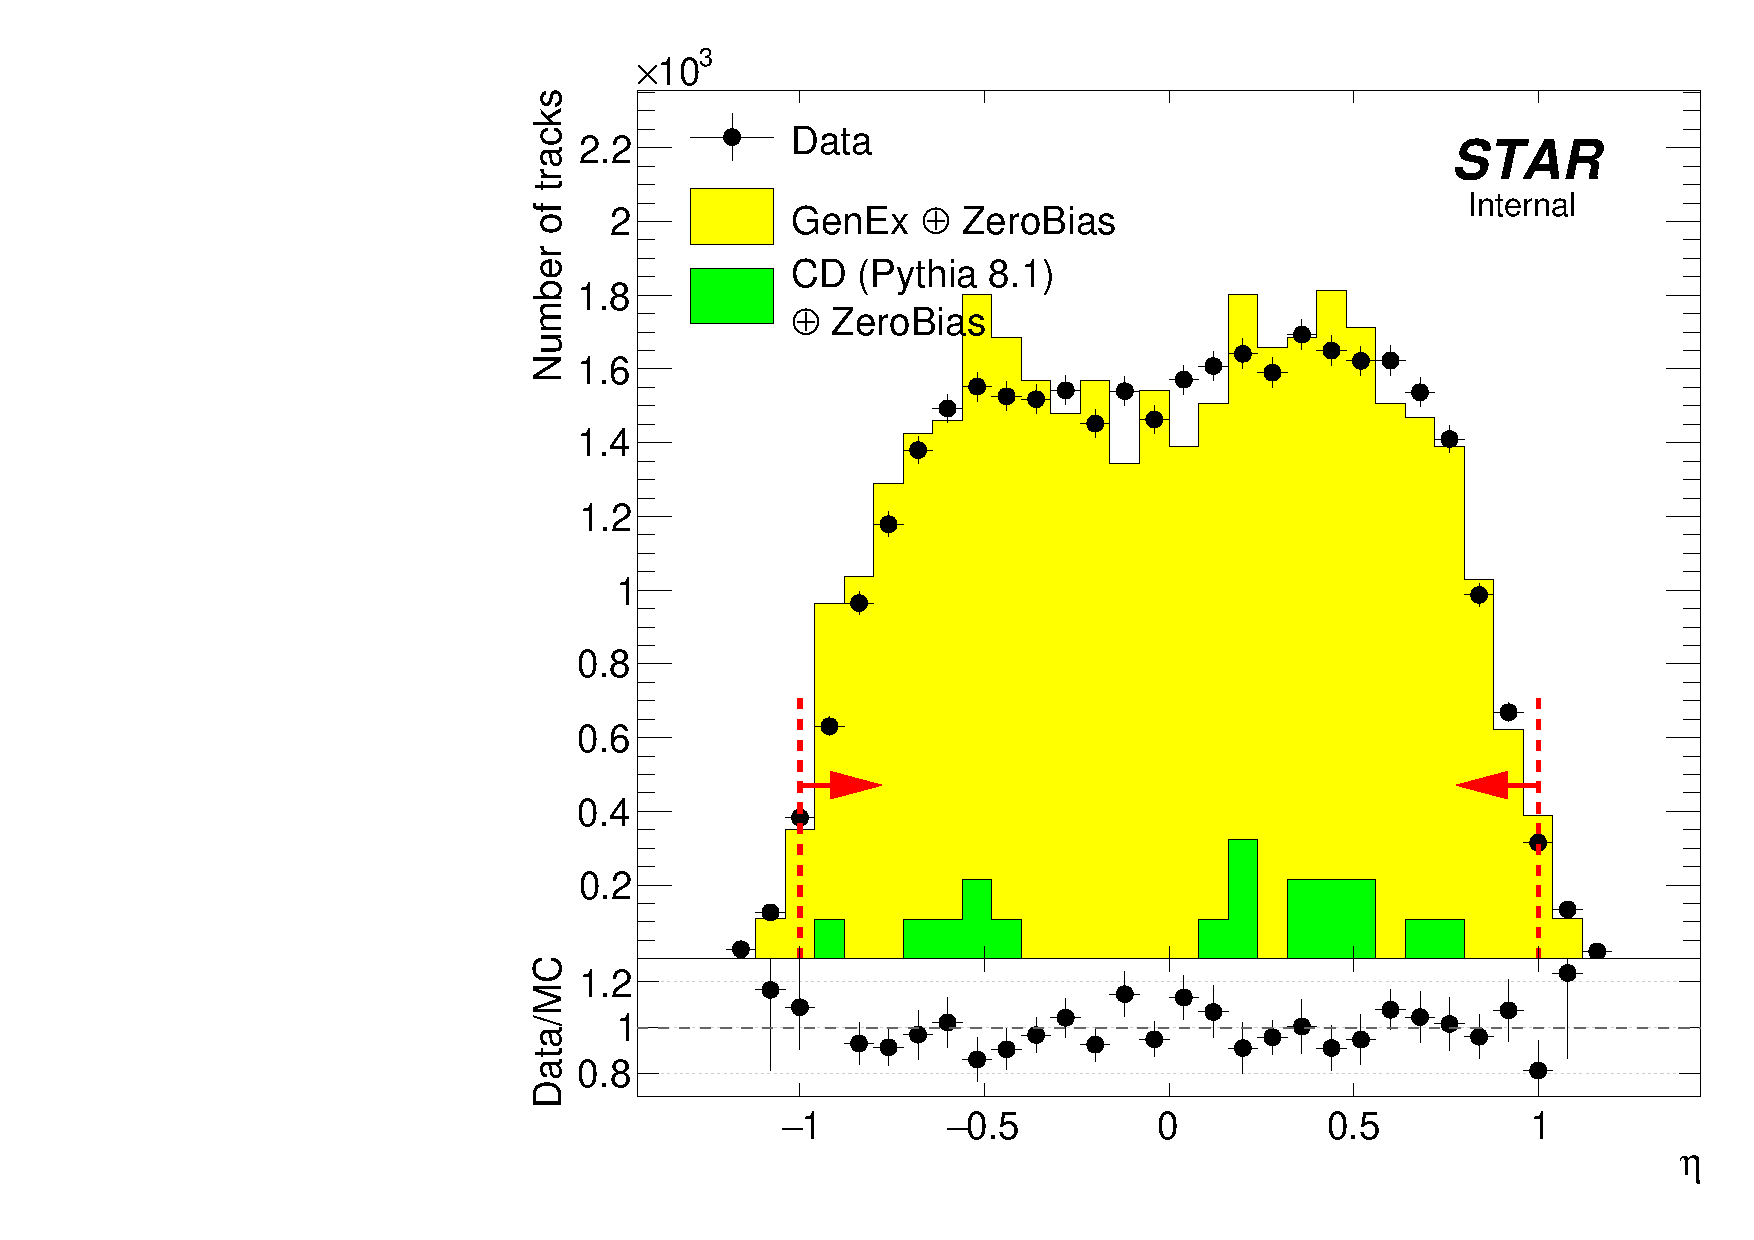
\includegraphics[width=\linewidth]{graphics/eventSelection/TpcTracks/TrackEta.pdf}}}
  \end{subfigure}
}%
\quad\quad%
\parbox{0.4725\textwidth}{%
  \centering
  \begin{subfigure}[b]{\linewidth}{
                \subcaptionbox{\label{fig:TrackPhi}}{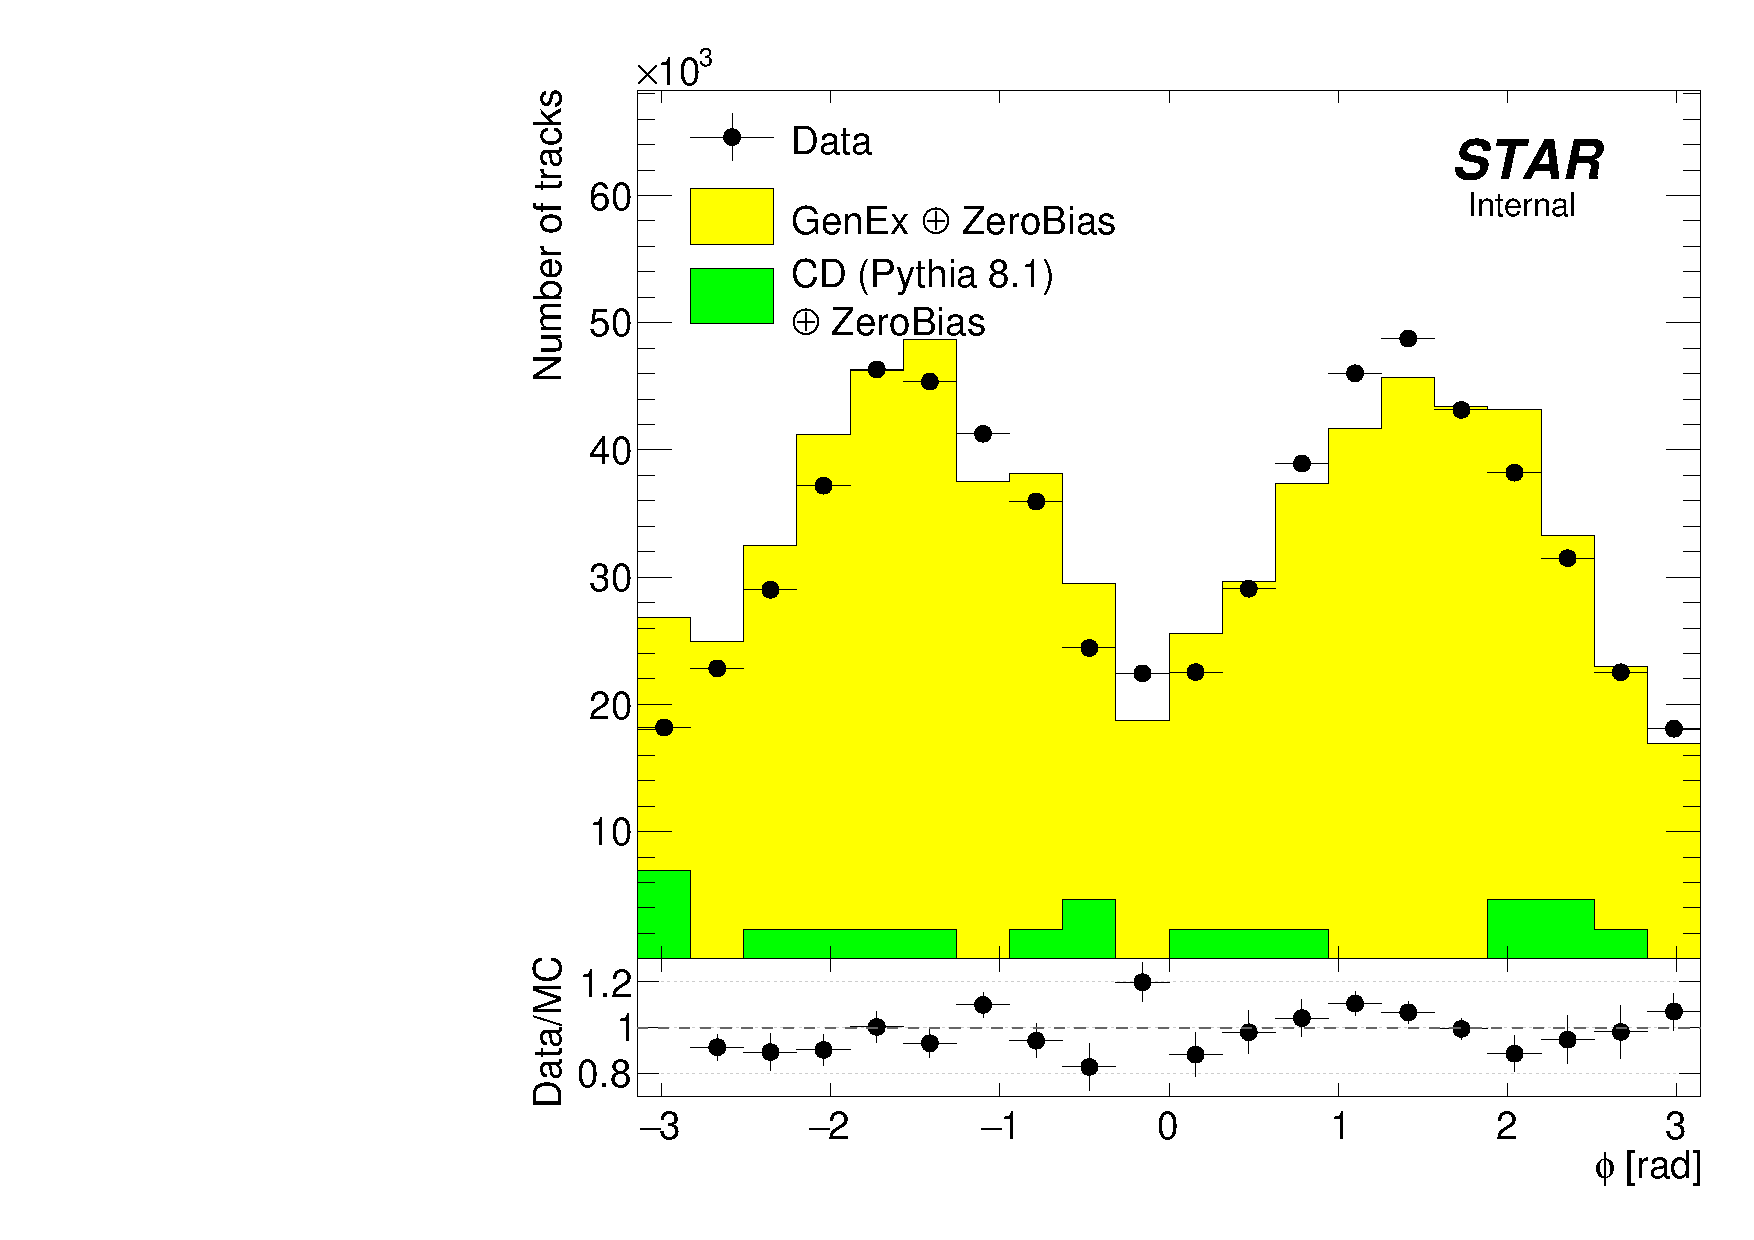
\includegraphics[width=\linewidth]{graphics/eventSelection/TpcTracks/TrackPhi.pdf}}}
  \end{subfigure}
}%
\caption[Comparison of distribution of track $\eta$ and $\phi$ in the data and embedded MC]
{Comparison of the track pseudorapidity $\eta$ (\ref{fig:TrackEta}) and the track azimuthal angle $\phi$ (\ref{fig:TrackPhi}) in the data and embedded MC. Normalizations of the signal and backgrounds were established from the comparison of $p_{T}^{\text{miss}}$ and $\Delta\theta$ distributions after full selection (without cut on the presented quantity and without exclusivity cut), as described in Sec.~\ref{sec:bkgdSignalNorm}. Red dashed lines and red arrows indicate the range of each quantity which is accepted in analysis.}\label{fig:TrackEtaPhi}
\end{figure}
%---------------------------









\subsection{(\ref{enum:CutRpTrks})~RP tracks}

%---------------------------
\begin{figure}[ht!]
\centering
\parbox{0.315\textwidth}{
  \centering
  \begin{subfigure}[b]{\linewidth}{
                \subcaptionbox{\label{fig:LocalAngles_2D}}{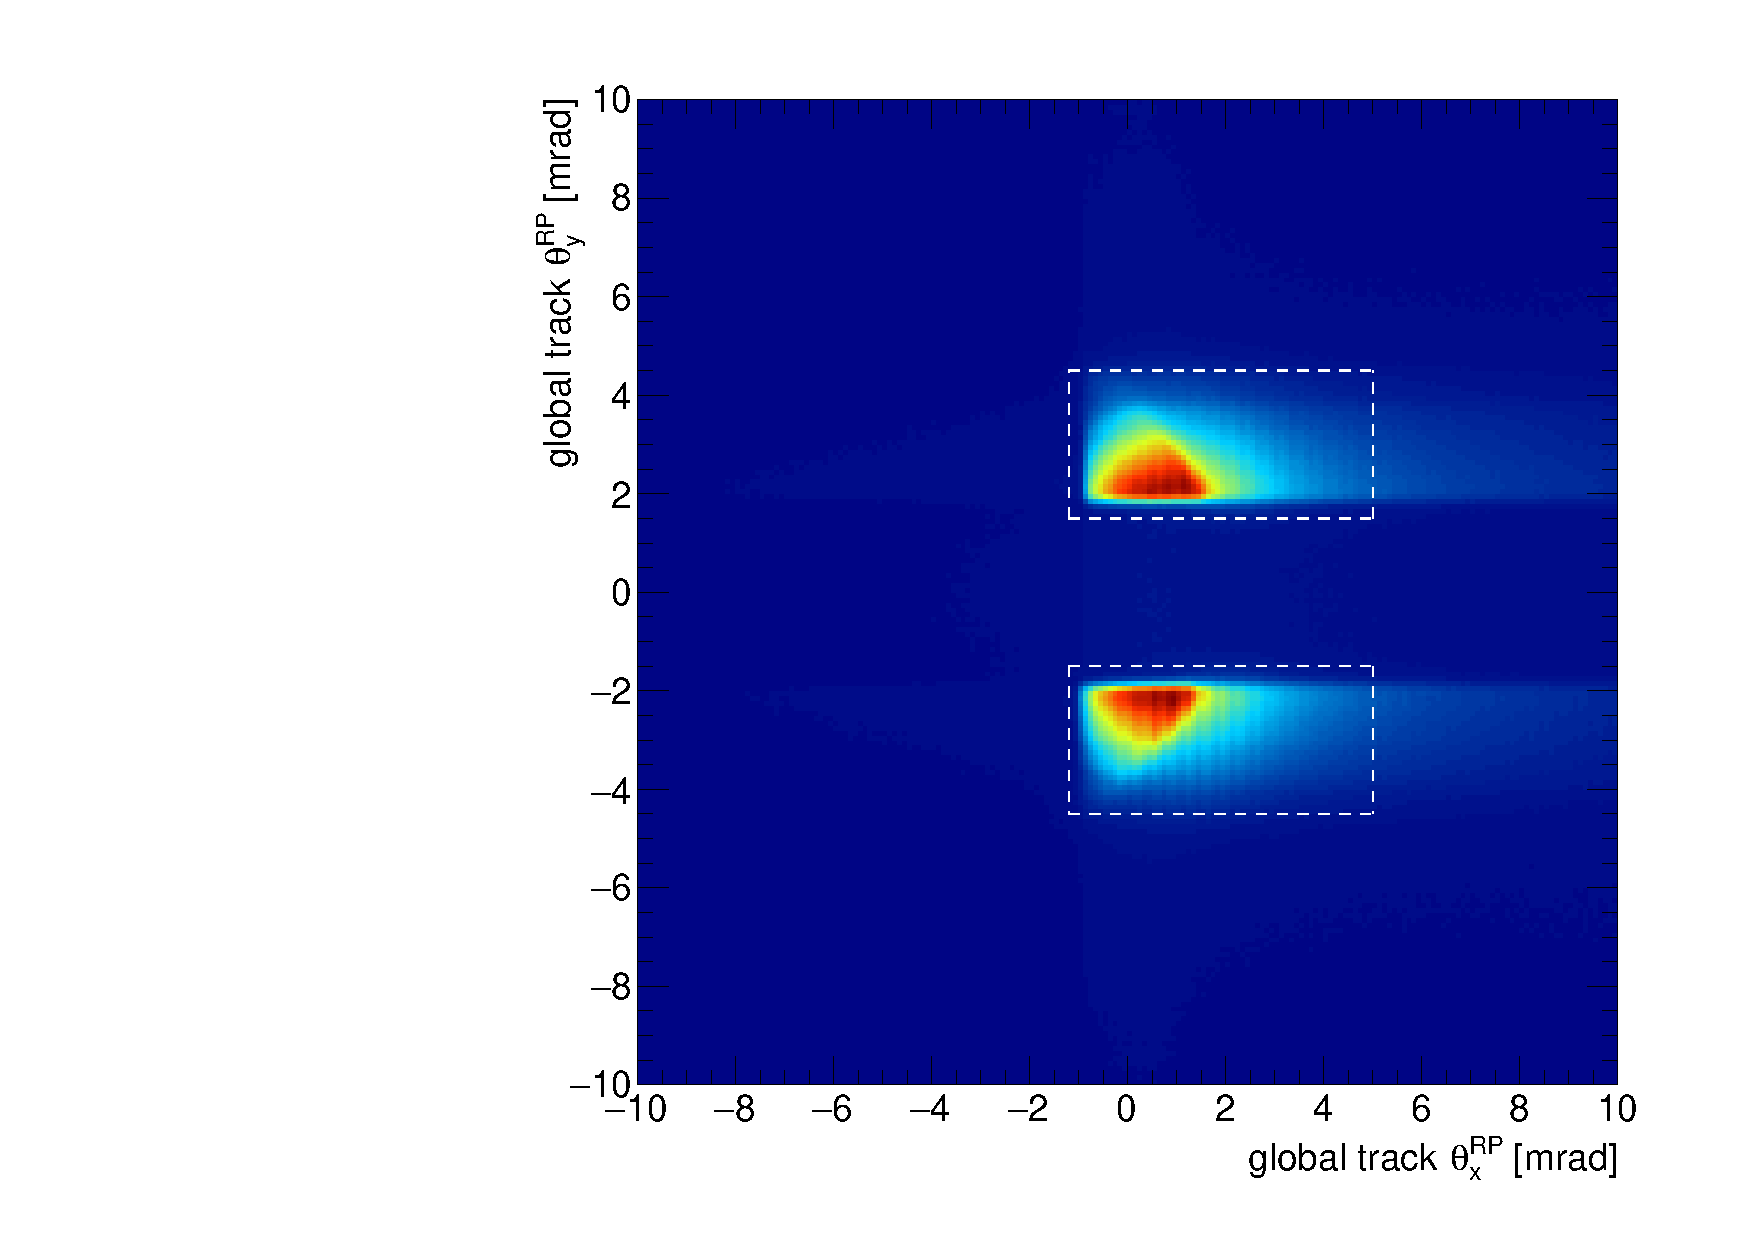
\includegraphics[width=\linewidth,page=1]{graphics/eventSelection/LocalAngles.pdf}}}
  \end{subfigure}
}
\quad
\parbox{0.315\textwidth}{
  \centering
  \begin{subfigure}[b]{\linewidth}{
                \subcaptionbox{\label{fig:LocalAngles_1D_x}}{\includegraphics[width=\linewidth,page=2]{graphics/eventSelection/LocalAngles.pdf}}}
  \end{subfigure}
}
\quad
\parbox{0.315\textwidth}{
  \centering
  \begin{subfigure}[b]{\linewidth}{
                \subcaptionbox{\label{fig:LocalAngles_1D_y}}{\includegraphics[width=\linewidth,page=3]{graphics/eventSelection/LocalAngles.pdf}}}
  \end{subfigure}
}%
\caption{Local angles of global tracks in Roman Pots.}
\end{figure}
%---------------------------



\subsection{(\ref{enum:CutDeltaZVx})~TPC-RP \texorpdfstring{$z$}{z}-vertex matching}


%---------------------------
\begin{figure}[ht!]
\centering
\parbox{0.4\textwidth}{
  \centering
  \begin{subfigure}[b]{\linewidth}{
                \subcaptionbox{\label{fig:zVertexRpVsTpc}}{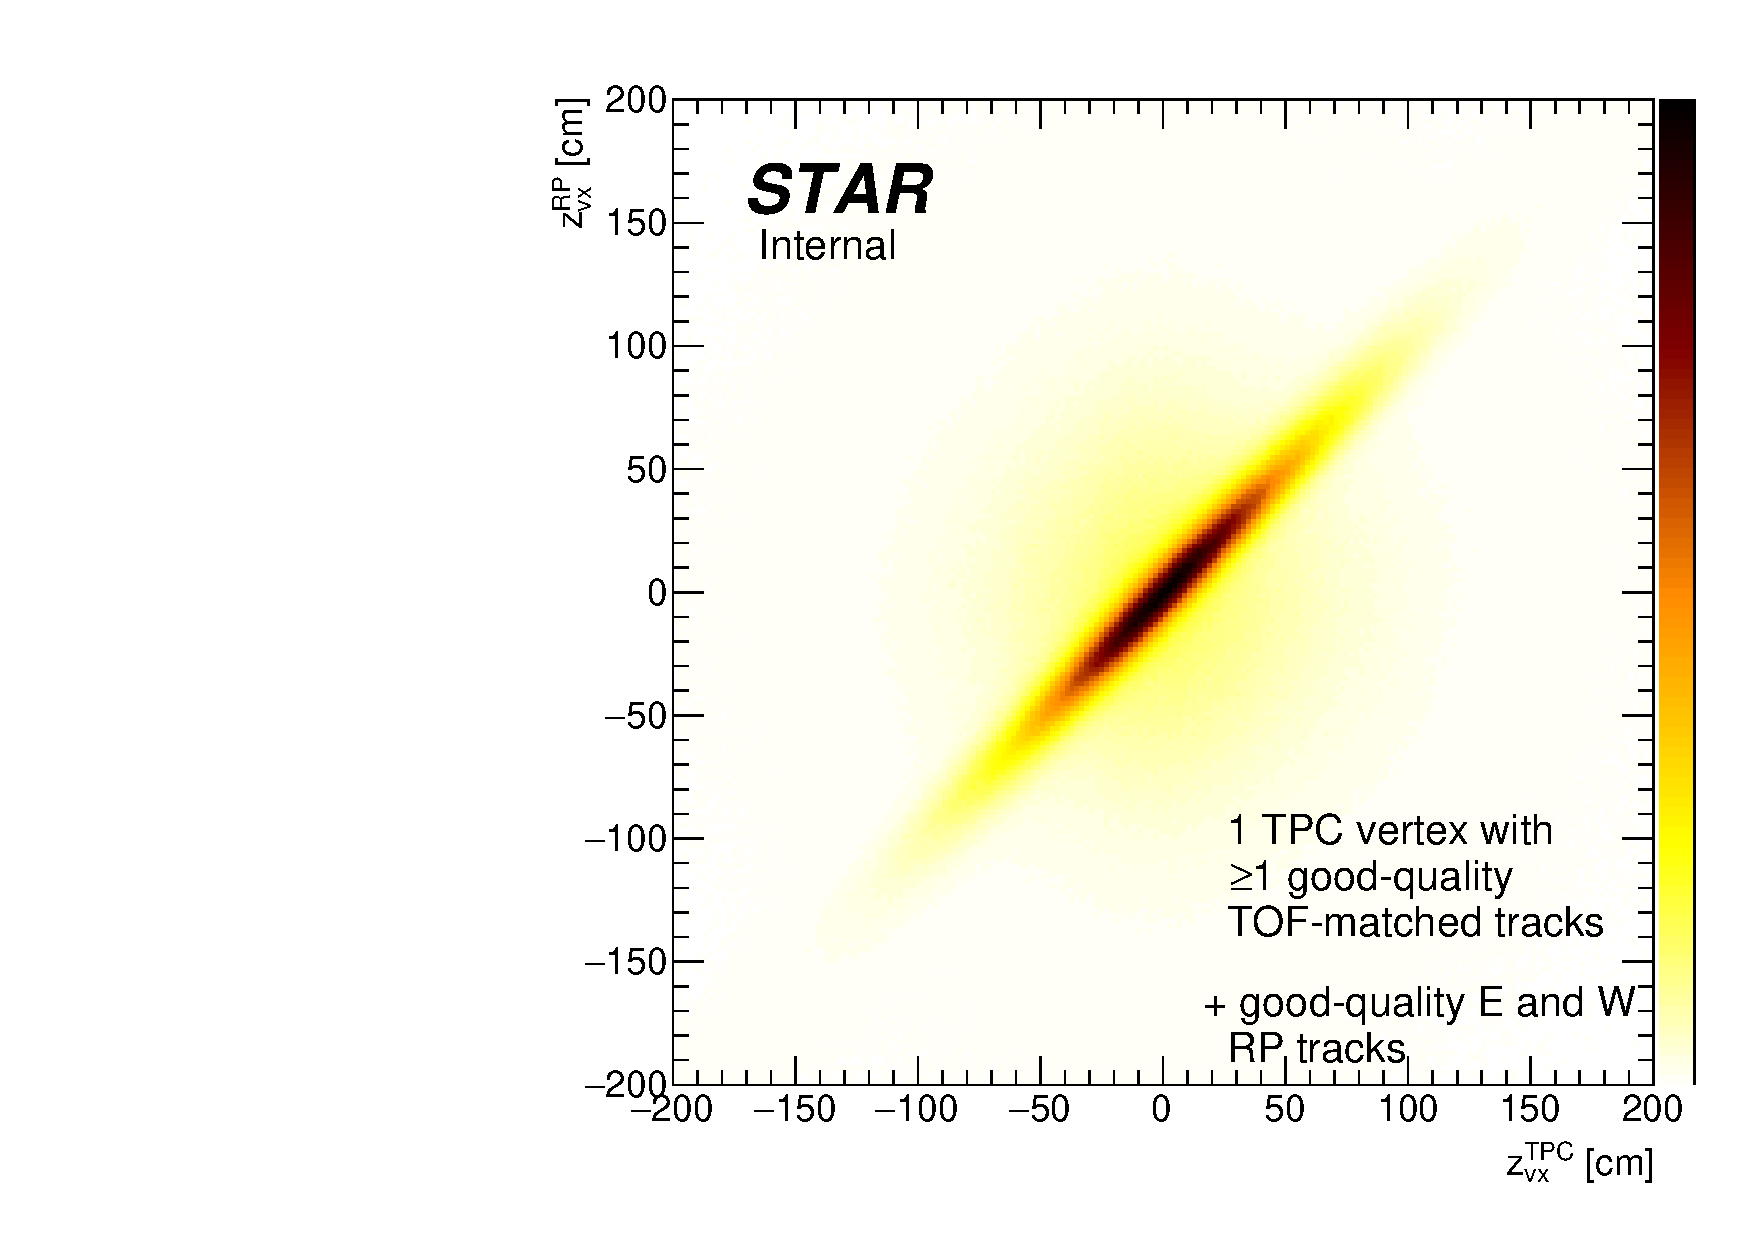
\includegraphics[width=\linewidth]{graphics/eventSelection/zVertexRpVsTpc.pdf}}}
  \end{subfigure}
}
\quad
\parbox{0.545\textwidth}{
  \centering
  \begin{subfigure}[b]{\linewidth}{
                \subcaptionbox{\label{fig:zVertexRpMinusZVertexTpc}}{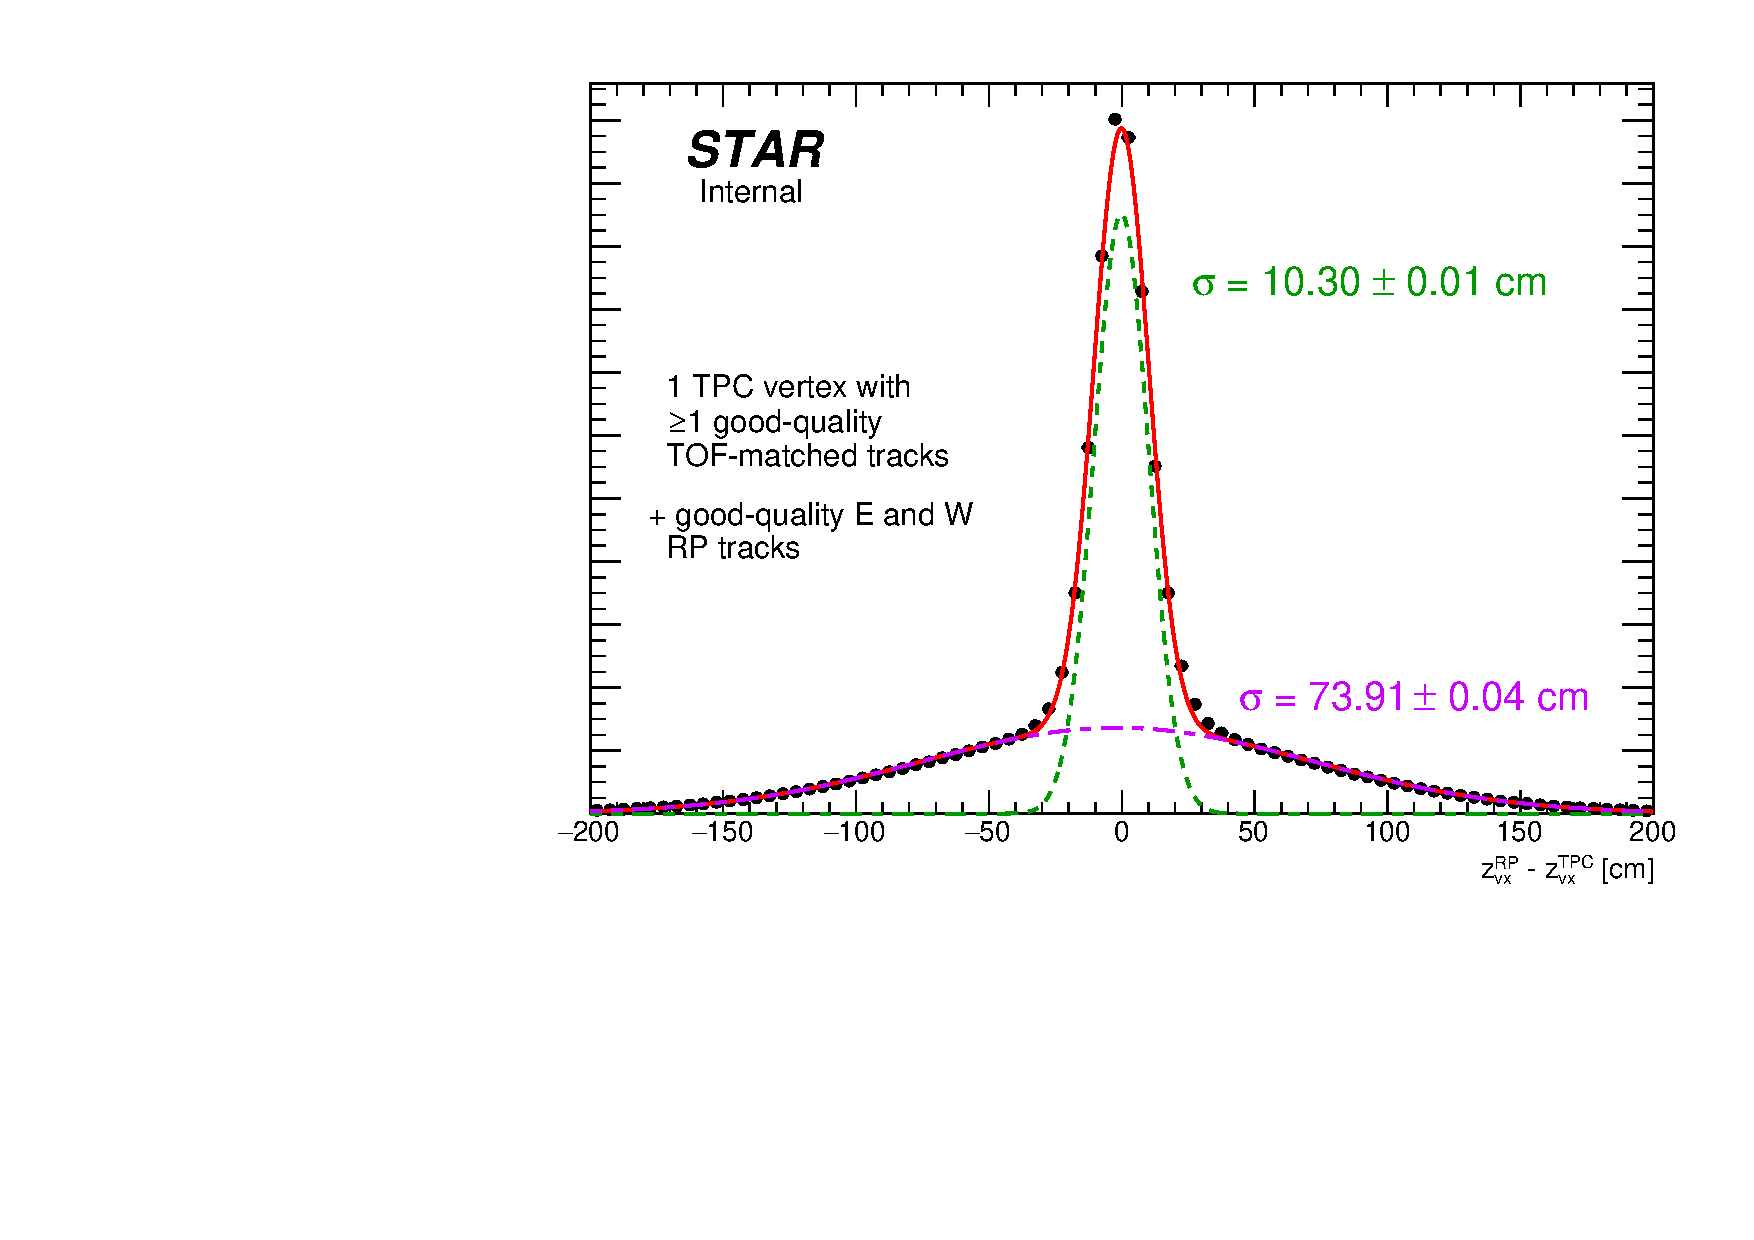
\includegraphics[width=\linewidth]{graphics/eventSelection/zVertexRpMinusZVertexTpc.pdf}}}
  \end{subfigure}
}%
\caption[Correlation and difference of $z$-vertex position measured in Roman Pots and TPC.]{Correlation (Fig.~\ref{fig:zVertexRpVsTpc}) and difference (Fig.~\ref{fig:zVertexRpMinusZVertexTpc}) of $z$-vertex position measured in Roman Pots and TPC.}
\end{figure}
%---------------------------


% %---------------------------
% \begin{figure}[ht!]
% % \begin{wrapfigure}{l}{0.475\textwidth}%[ht!]
% \centering%
% 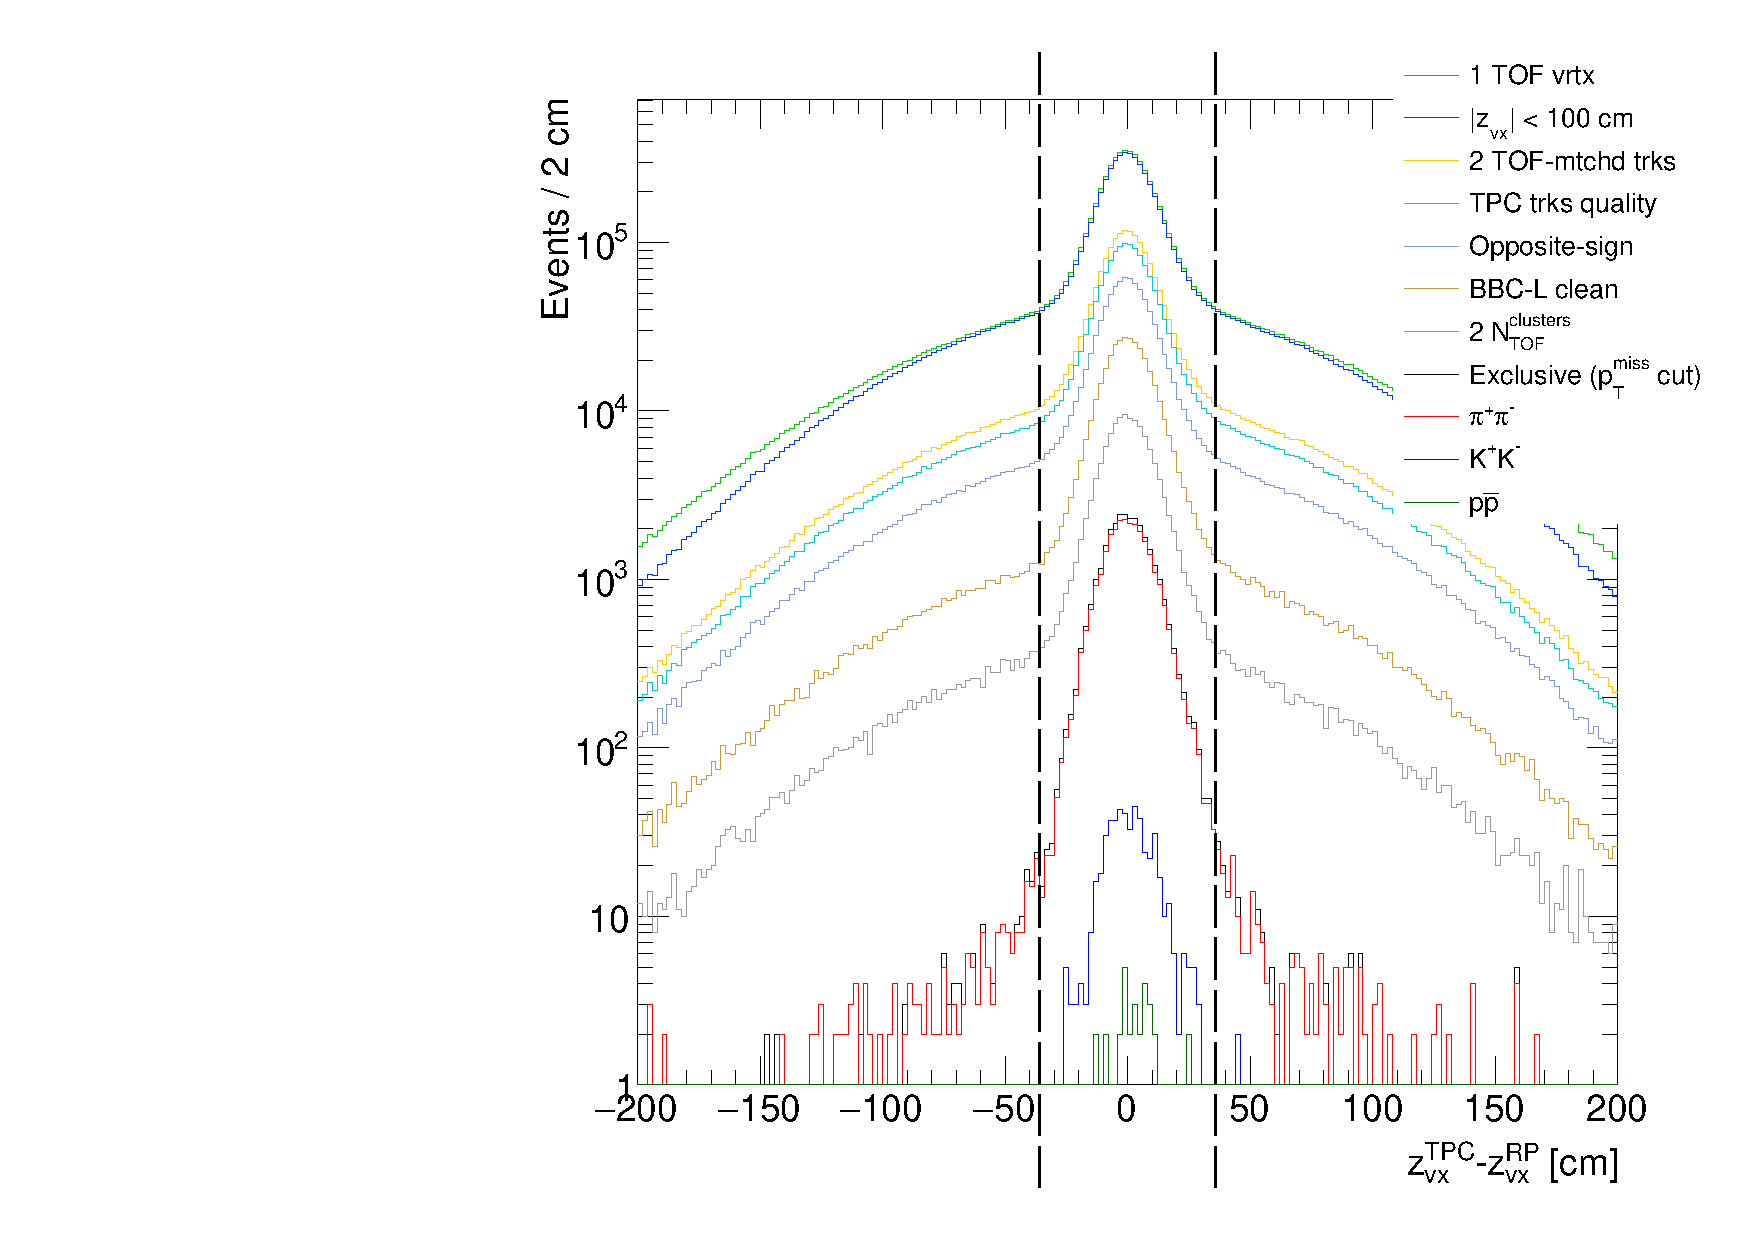
\includegraphics[width=0.475\linewidth,page=1]{graphics/eventSelection/DeltaZVx.pdf}%
% % % 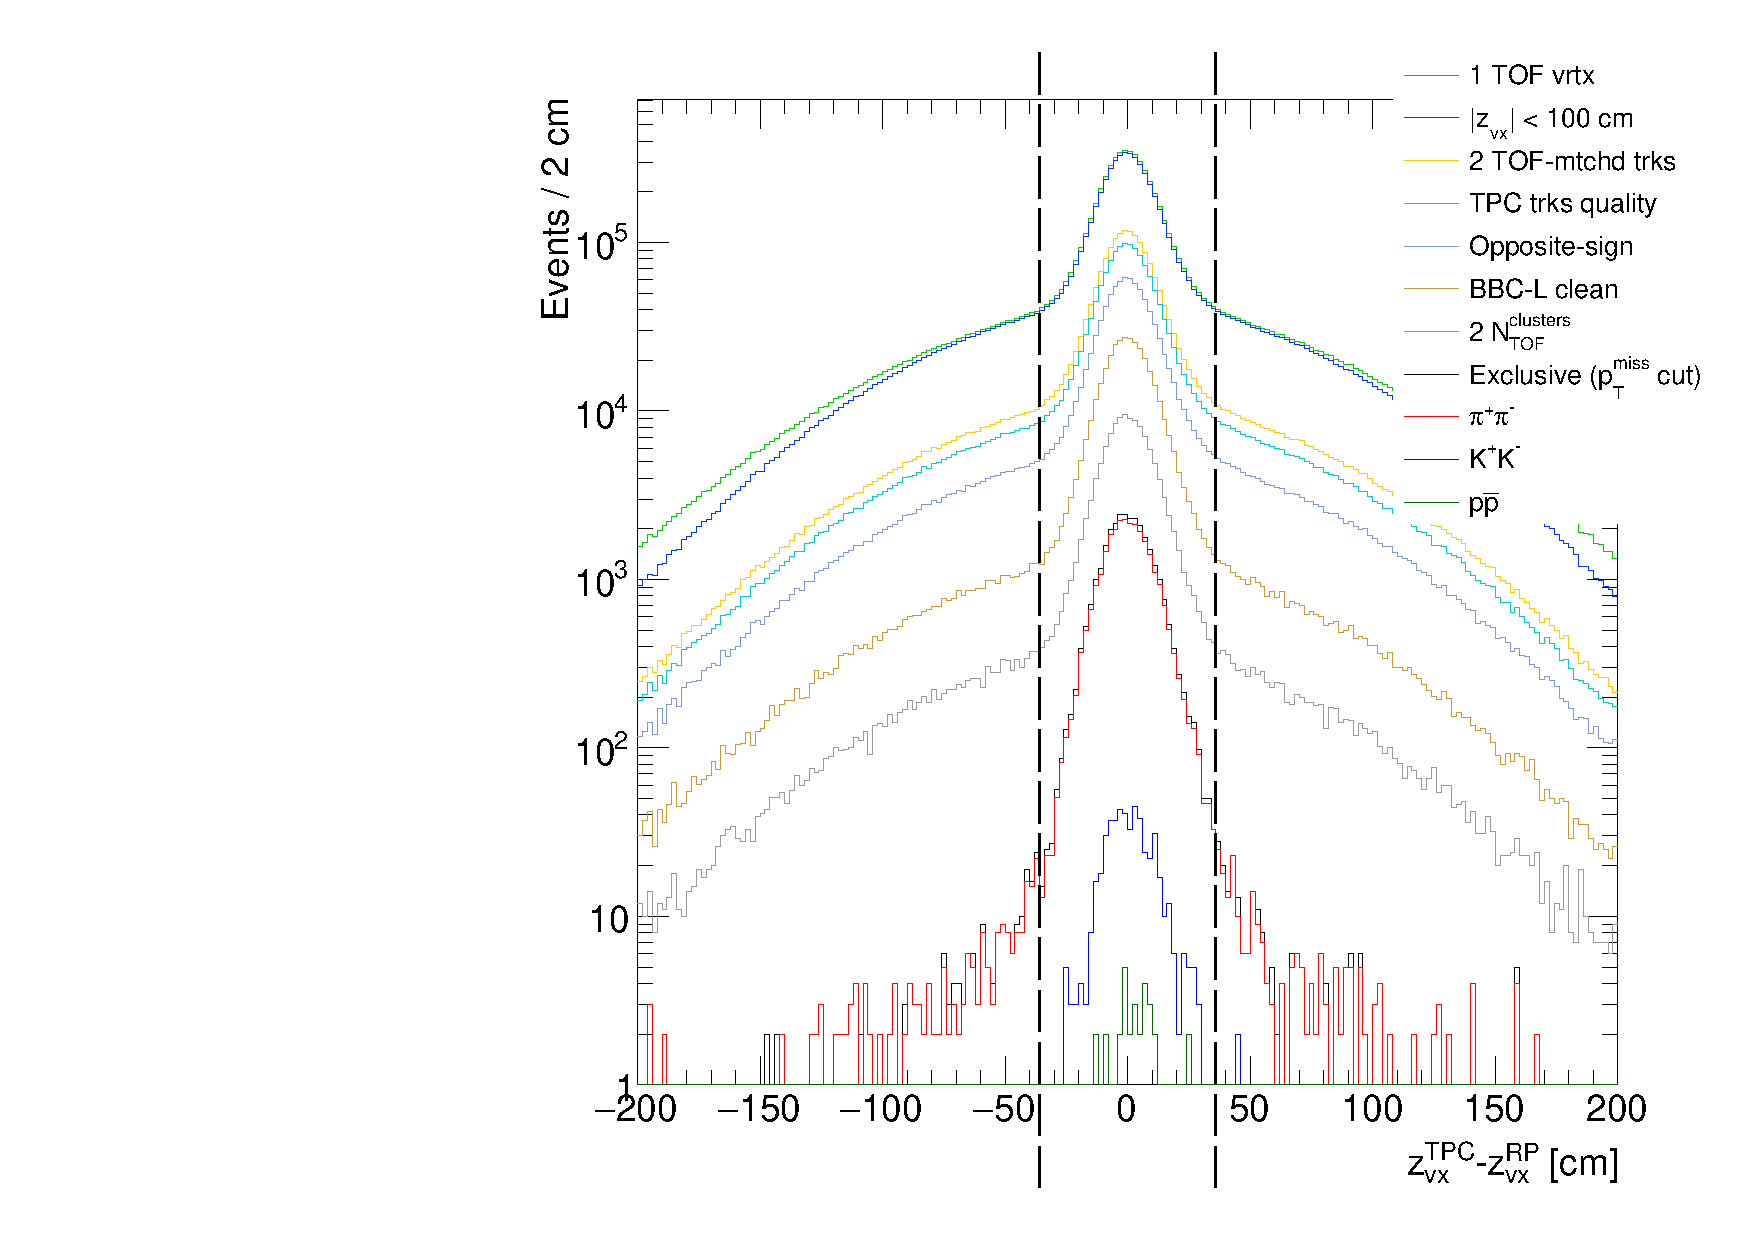
\includegraphics[width=\linewidth,page=1]{graphics/eventSelection/DeltaZVx.pdf}%
% \caption{Delta z-vx.}\label{fig:DeltaZVx}%
% \end{figure}
% % \end{wrapfigure}
% %---------------------------
%%%%%%%%%%%%%%%%%%%%%%%%%%%%%%%%%%%%%%%%%%%%%%%%%%%%%%%%%%%%%%%%%%%%%%%%%%%%%%%%%%%%%%%%%%%%%%%%%%%%%%%%%%%%%%%%%%%%%%%%%%%%%%%%%%%%




%%%%%%%%%%%%%%%%%%%%%%%%%%%%%%%%%%%%%%%%%%%%%%%%%%%%%%%%%%%%%%%%%%%%%%%%%%%%%%%%%%%%%%%%%%%%%%%%%%%%%%%%%%%%%%%%%%%%%%%%%%%%%%%%%%%%
\subsection{(\ref{enum:CutBbcLarge})~BBC-large signal veto}

At the trigger level a veto on signal in small BBC detectors was used. During offline analysis we found that the non-exclusive background can be efficiently rejected if an additional veto on signal in large BBC detectors is added. It is connected with the fact that vast majority of selected RP\_CPT2 triggers were from the central diffraction process to which CEP belongs. Many of central diffraction events have particles produced in the rapidity region outside the TPC and TOF acceptance, some hitting large BBC tiles. Presence of signal in large BBC is therefore a signature of background or a pile-up interaction.

The response of large BBC tiles is different from that of small BBC tiles, as shown in sample plots in Fig.~\ref{fig:sampleBbcResponse} (similar distributions for all channels can be found in Appendix~\ref{appendix:bbc}). Typically in small BBC tiles a peak visible in ADC distribution around $100-150$ (Figs.~\ref{fig:sampleBbcSmallAdcVsTac},\ref{fig:sampleBbcSmallAdc}), a signature of good separation of the electronics noise and signal from the ionizing particle. No such feature is observed in corresponding distribution for large BBC tile (Figs.~\ref{fig:sampleBbcLargeAdcVsTac},\ref{fig:sampleBbcLargeAdc}), which can be explained by the difference in geometry (in size) of small and large tiles. In large BBC tiles the path that scintillation light must travel to reach PMT is much longer in comparison to smal BBC tiles (multiple reflections on the main tile surface due to small thickness of the tile) therefore it is highly attenuated and extended in time. This is possible reason of lack of signal peak in the ADC distribution in large BBC tile spectrum (Fig.~\ref{fig:sampleBbcLargeAdc}), as well as the late-TAC (TAC$<\sim600$, ADC$<100$) tail in the ADC vs. TAC spectrum (slewing effect, Fig.~\ref{fig:sampleBbcLargeAdcVsTac}). Nevertheless, the above features of BBC-large response does not disqualify this detector from being used as a veto detector, as in this case lower efficiency of the detector only reduce the background rejection power.


%---------------------------
\begin{figure}[h]
\centering
\parbox{0.4725\textwidth}{
  \centering
  \begin{subfigure}[b]{\linewidth}
                \subcaptionbox{\label{fig:sampleBbcSmallAdcVsTac}}{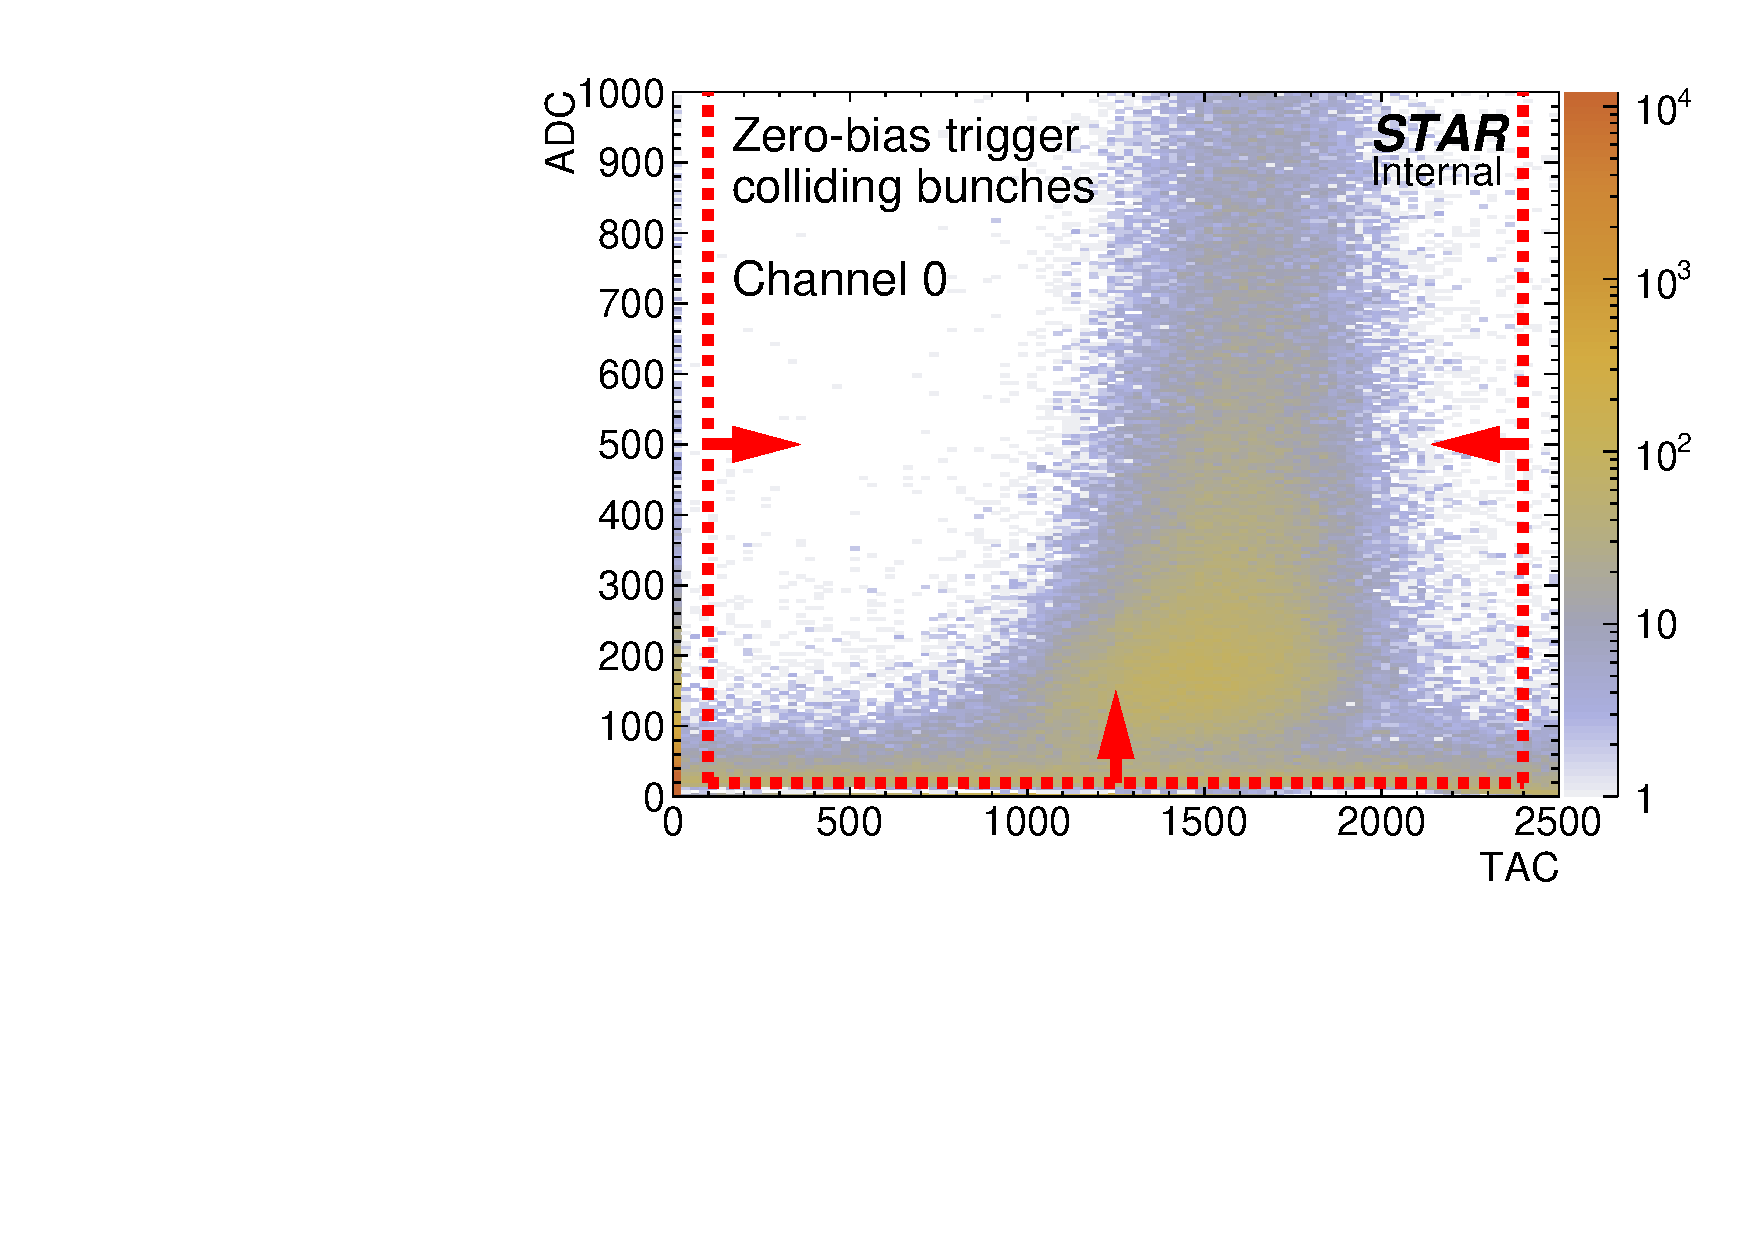
\includegraphics[width=\linewidth,page=1]{graphics/eventSelection/bbc/Bbc_ADCvsTAC_collidingBunches.pdf}}
  \end{subfigure}\\
  \begin{subfigure}[b]{\linewidth}\addtocounter{subfigure}{1}
                \subcaptionbox{\label{fig:sampleBbcSmallAdc}}{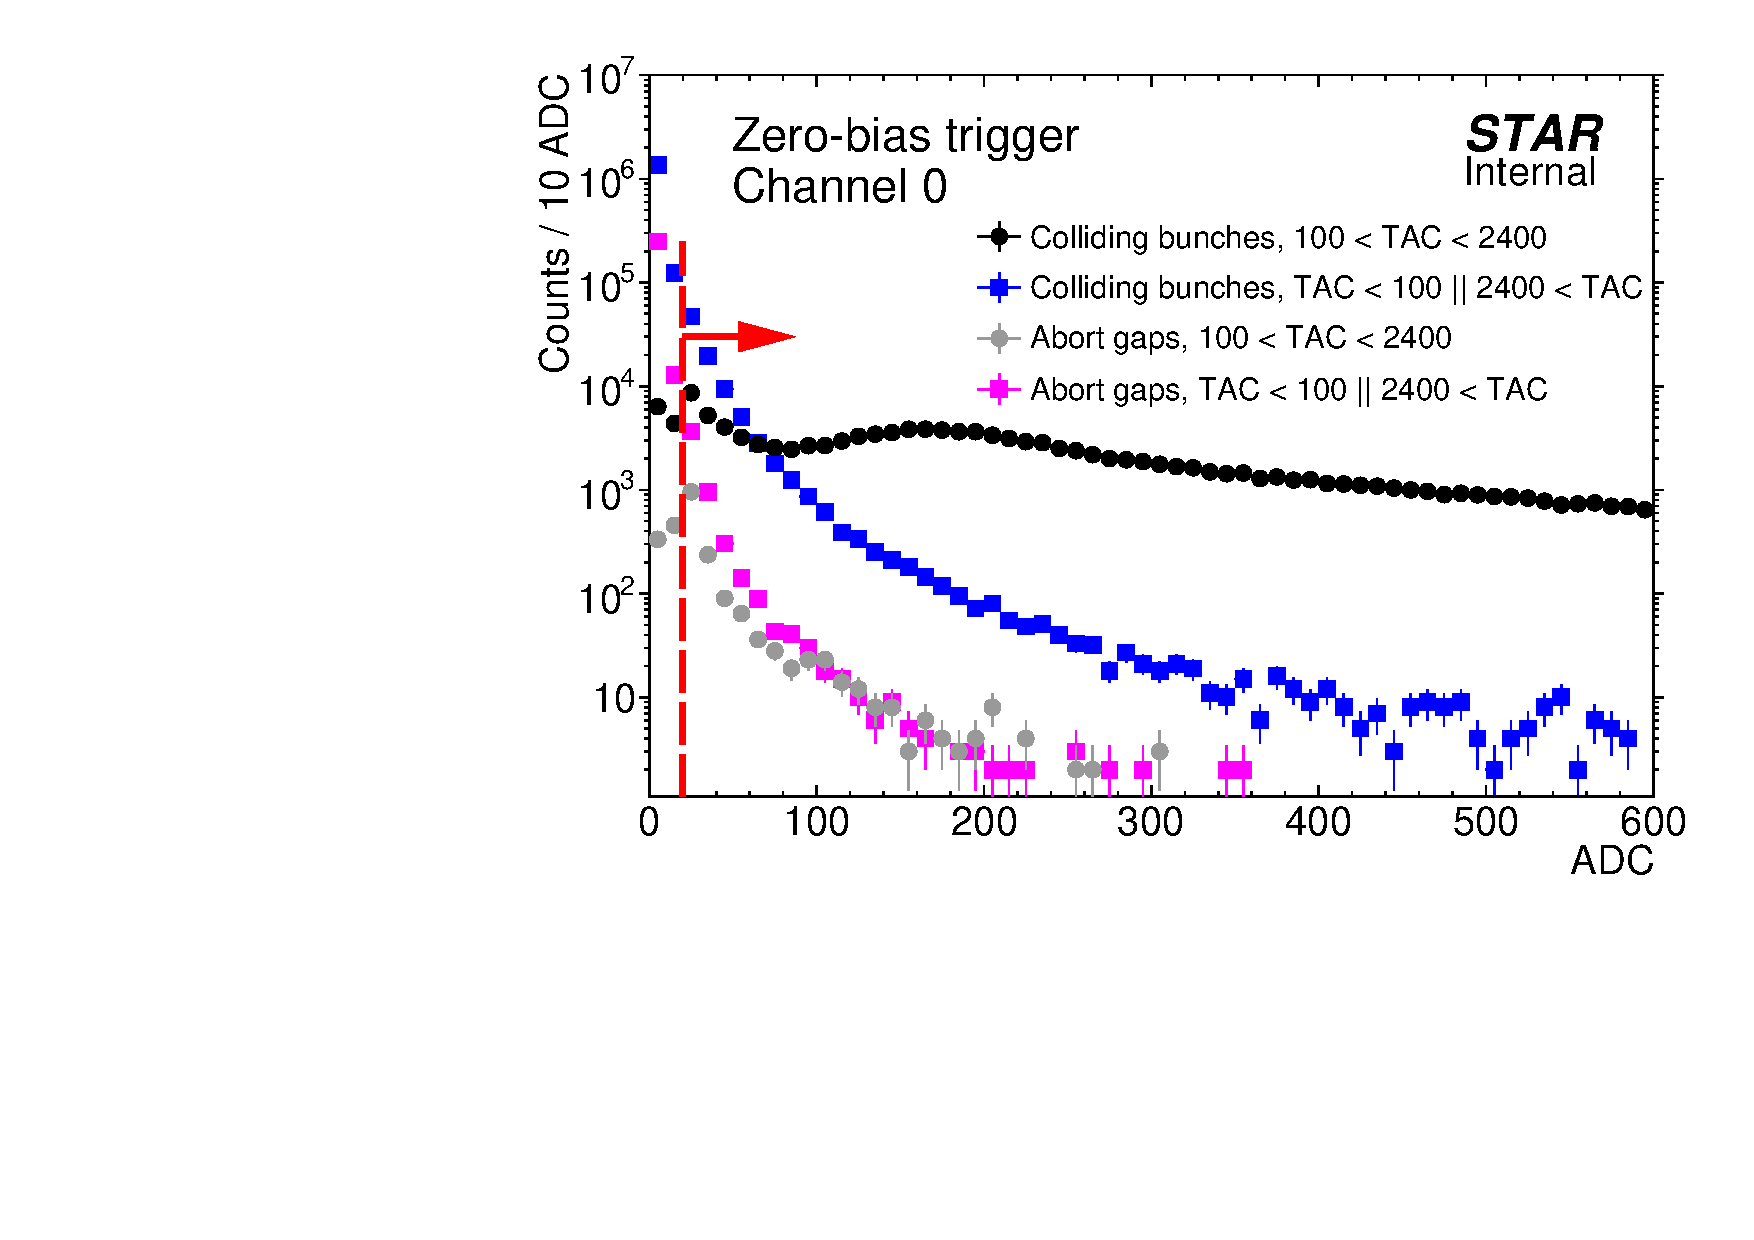
\includegraphics[width=\linewidth,page=1]{graphics/eventSelection/bbc/Bbc_ADC.pdf}}
  \end{subfigure}
}%
\quad\quad%
\parbox{0.4725\textwidth}{
  \centering
  \begin{subfigure}[b]{\linewidth}\addtocounter{subfigure}{-2}
                \subcaptionbox{\label{fig:sampleBbcLargeAdcVsTac}}{\includegraphics[width=\linewidth,page=17]{graphics/eventSelection/bbc/Bbc_ADCvsTAC_collidingBunches.pdf}}
  \end{subfigure}\\
  \begin{subfigure}[b]{\linewidth}\addtocounter{subfigure}{1}
                \subcaptionbox{\label{fig:sampleBbcLargeAdc}}{\includegraphics[width=\linewidth,page=17]{graphics/eventSelection/bbc/Bbc_ADC.pdf}}
  \end{subfigure}
}%
\label{fig:sampleBbcResponse}%
\caption[Sample BBC-small and BBC-large response in zero-bias triggers.]{Sample BBC-small (left column) and BBC-large (right column) response in zero-bias data. Top row shows TAC vs. ADC distributions, bottom row shows projection of the corresponding two-dimensional ditribution on $x$-axis (ADC) in the TAC range quoted in the legend, for both abort gaps and colliding bunches. Red lines and arrows indicate thresholds for a signal in presented channels.}
\end{figure}
%---------------------------


Each channel of the BBC-large has different response to signal from ionizing particle, as well as different level of noise. We decided to set up a signal threshold for each channel based on a study of the noise in abort gaps (in zero-bias data). This noise, in principle, should be solely the electronics noise. We checked for each channel the probability to detect a signal with ADC above certain threshold and with TAC contained within 100 and 2400 (the same window is deafult for small BBC). The result is shown in Fig.~\ref{fig:bbcLargeThresholds}. Next, we established final ADC thresholds in each BBC-large channel by requiring that the noise in BBC-large would cause a veto in maximally $3.5\%$ of events. To transform it to $\text{ADC}_{thr}$ we first assumed that the noise is uncorrelated between the channels. With this assumption one can connect the probability of the veto in whole BBC-large detector (east and west) caused by noise $\mathcal{P}_{\text{veto}}^{\text{noise}}$ with the probability of the signal induced by noise in single BBC-large channel $\mathcal{P}_{i,\text{sig}}^{\text{noise}}$:
\begin{equation}\label{eq:bbcNoise1}
 \mathcal{P}_{\text{veto}}^{\text{noise}} = 1-\mathcal{P}_{!\text{veto}}^{\text{noise}} = 1-\left( 1-\mathcal{P}_{i,\text{sig}}^{\text{noise}} \right)^{N^{\text{BBC}}_{\text{ch}}}.
\end{equation}
In the equation above $N^{\text{BBC}}_{\text{ch}}$ denotes number of active channels in BBC-large. From plots contained in Appendix~\ref{appendix:bbc} one can read that there were 14 active channels in BBC-large. 2 dead channels were found on the west side (40 and 42). By transforming Eq.~\ref{eq:bbcNoise1} to the form presented below we can calculate the threshold probability for a single BBC-large channel:
\begin{equation}\label{eq:bbcNoise2}
 \mathcal{P}_{i,\text{sig}}^{\text{noise}} = 1-\sqrt[N^{\text{BBC}}_{\text{ch}}]{1-\mathcal{P}_{\text{veto}}^{\text{noise}}} = 1-\sqrt[14]{1-0.035} \approx 0.0025.
\end{equation}
In the last step we translated this number to ADC threshold for each channel of BBC-large. For this purpose we used Fig.~\ref{fig:bbcLargeThresholds}. The $x$-axis projection of the crossing point of each color line with the $y$-axis value of 0.0025 defines $\text{ADC}_{thr}$ for each particular channel. These numbers are listed in Tab.~\ref{tab:bbcLargeThresholds}. The event was dropped from analysis if any of the BBC-large channels registered signal of strength $\text{ADC}_{i}>\text{ADC}_{i,thr}$ and $100<\text{TAC}_{i}<2400$.



\begin{table}[h]
	\begin{minipage}{0.65\linewidth}
		\centering
		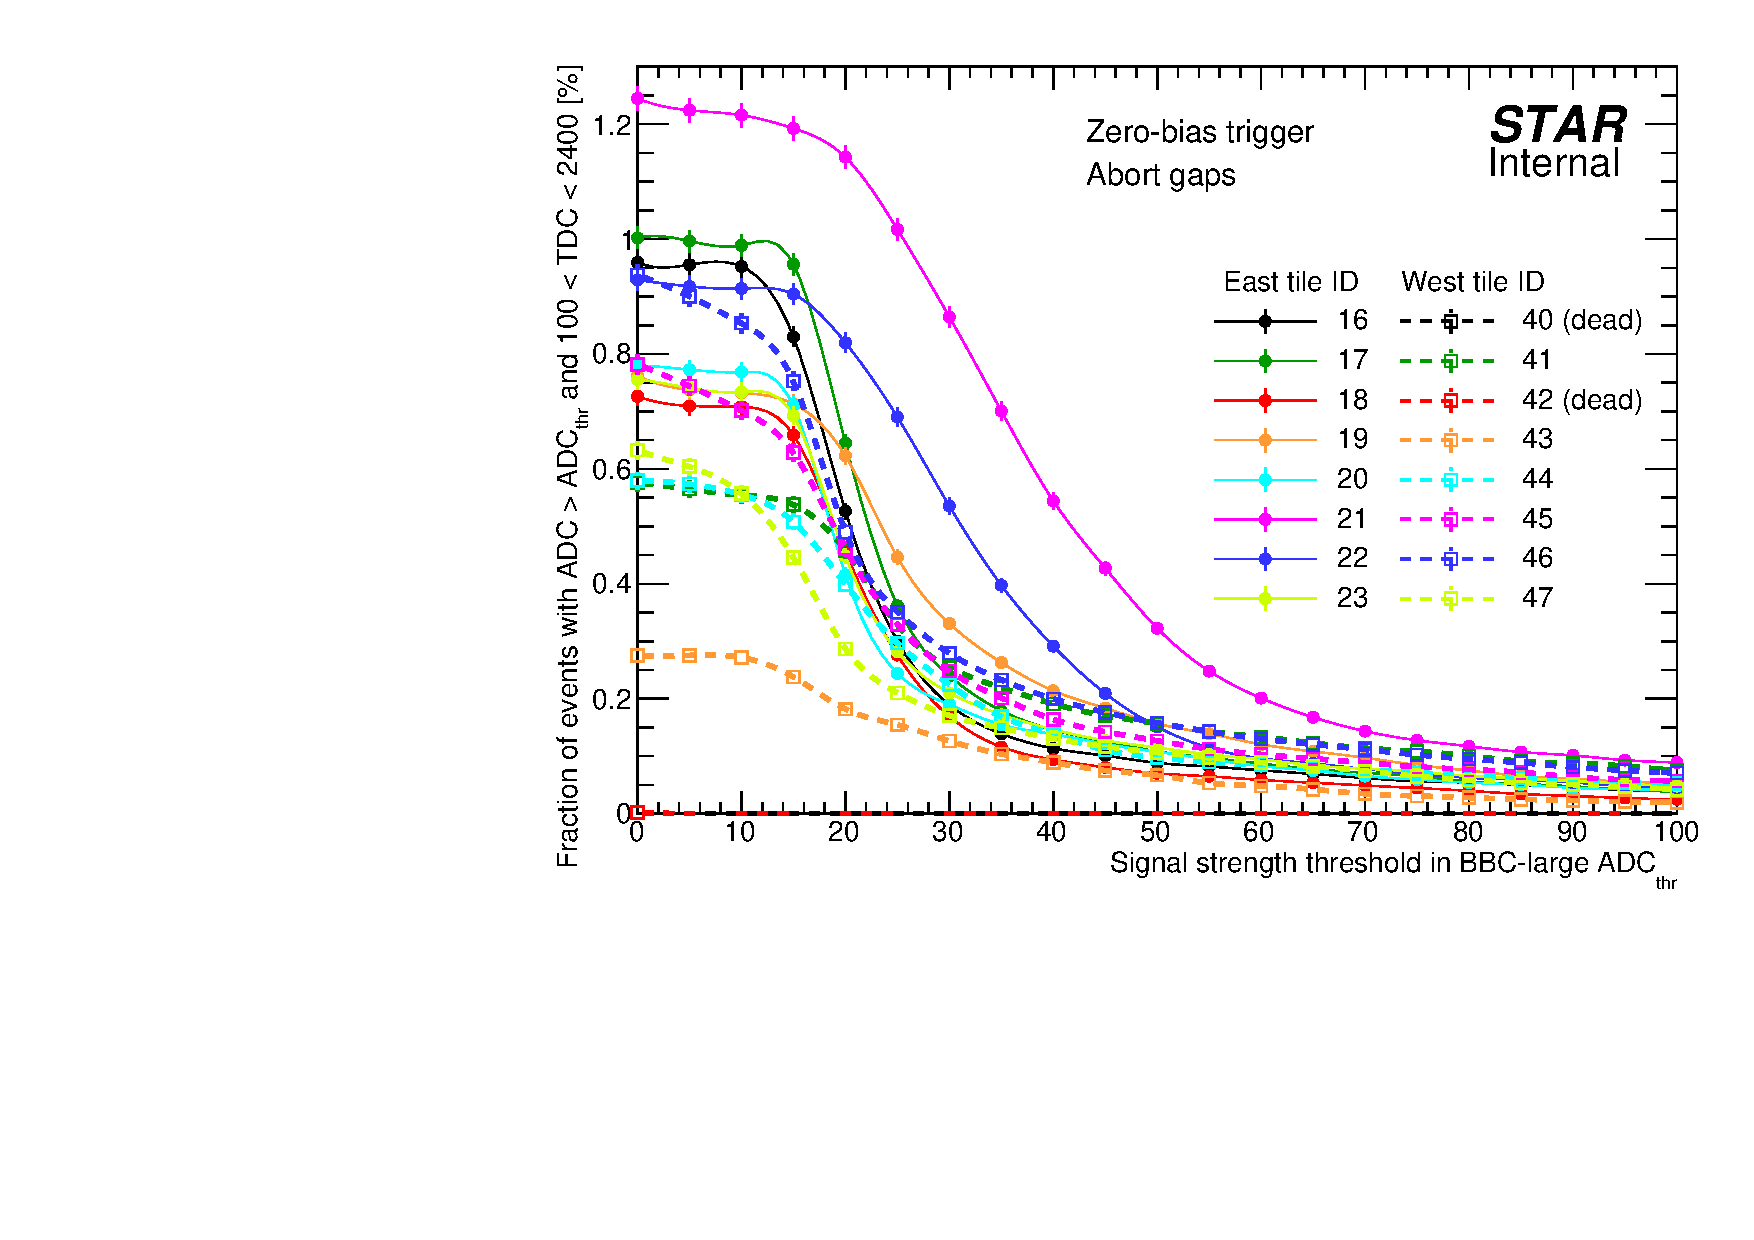
\includegraphics[width=\linewidth]{graphics/eventSelection/bbc/BbbLargeThreshold.pdf}
		\captionof{figure}[Probability of false BBC-large signal (noise-induced).]{Percentage of events in abort gaps from zero-bias triggers with the ADC counts larger than the ADC threshold given in the $x$-axis, for each BBC-large channel. Measured points with statistical uncertainties are connected with a smooth line of corresponding color for better visualization.}
		\label{fig:bbcLargeThresholds}
	\end{minipage}\hfill
	\begin{minipage}{0.3\linewidth}
		\centering
		\begin{tabular}{c|c||c|c}
			\multicolumn{2}{c||}{East} & \multicolumn{2}{c}{West} \\ \hline
			$i$  & $\text{ADC}_{\text{thr}}$ & $i$  & $\text{ADC}_{\text{thr}}$ \\ \hline
			16 & 27 & 40 & 0 \\
			17 & 30 & 41 & 31 \\
			18 & 26 & 42 & 0 \\
			19 & 37 & 43 & 14 \\
			20 & 25 & 44 & 29 \\
			21 & 55 & 45 & 30 \\
			22 & 43 & 46 & 33 \\
			23 & 27 & 47 & 22 \\
		\end{tabular}
		\caption[Offline ADC thresholds in BBC-large.]{Offline ADC thresholds in BBC-large.\newline\newline\newline\newline\newline\newline\newline\newline}
		\label{tab:bbcLargeThresholds}
	\end{minipage}

\end{table}

Observation of high purification of CEP sample with described BBC-large veto in the data from run 15 was helpful to improve the CEP trigger for run 17. The improved trigger called RP\_CPT2noBBCL was similar to RP\_CPT2 with an addition of BBC-large veto using ADC threshold of 50.

%%%%%%%%%%%%%%%%%%%%%%%%%%%%%%%%%%%%%%%%%%%%%%%%%%%%%%%%%%%%%%%%%%%%%%%%%%%%%%%%%%%%%%%%%%%%%%%%%%%%%%%%%%%%%%%%%%%%%%%%%%%%%%%%%%%%



%%%%%%%%%%%%%%%%%%%%%%%%%%%%%%%%%%%%%%%%%%%%%%%%%%%%%%%%%%%%%%%%%%%%%%%%%%%%%%%%%%%%%%%%%%%%%%%%%%%%%%%%%%%%%%%%%%%%%%%%%%%%%%%%%%%%
\subsection{(\ref{enum:CutTofClusters})~TOF clusters limit}

%---------------------------
\begin{figure}[ht!]
% \begin{wrapfigure}{l}{0.475\textwidth}%[ht!]
\centering%
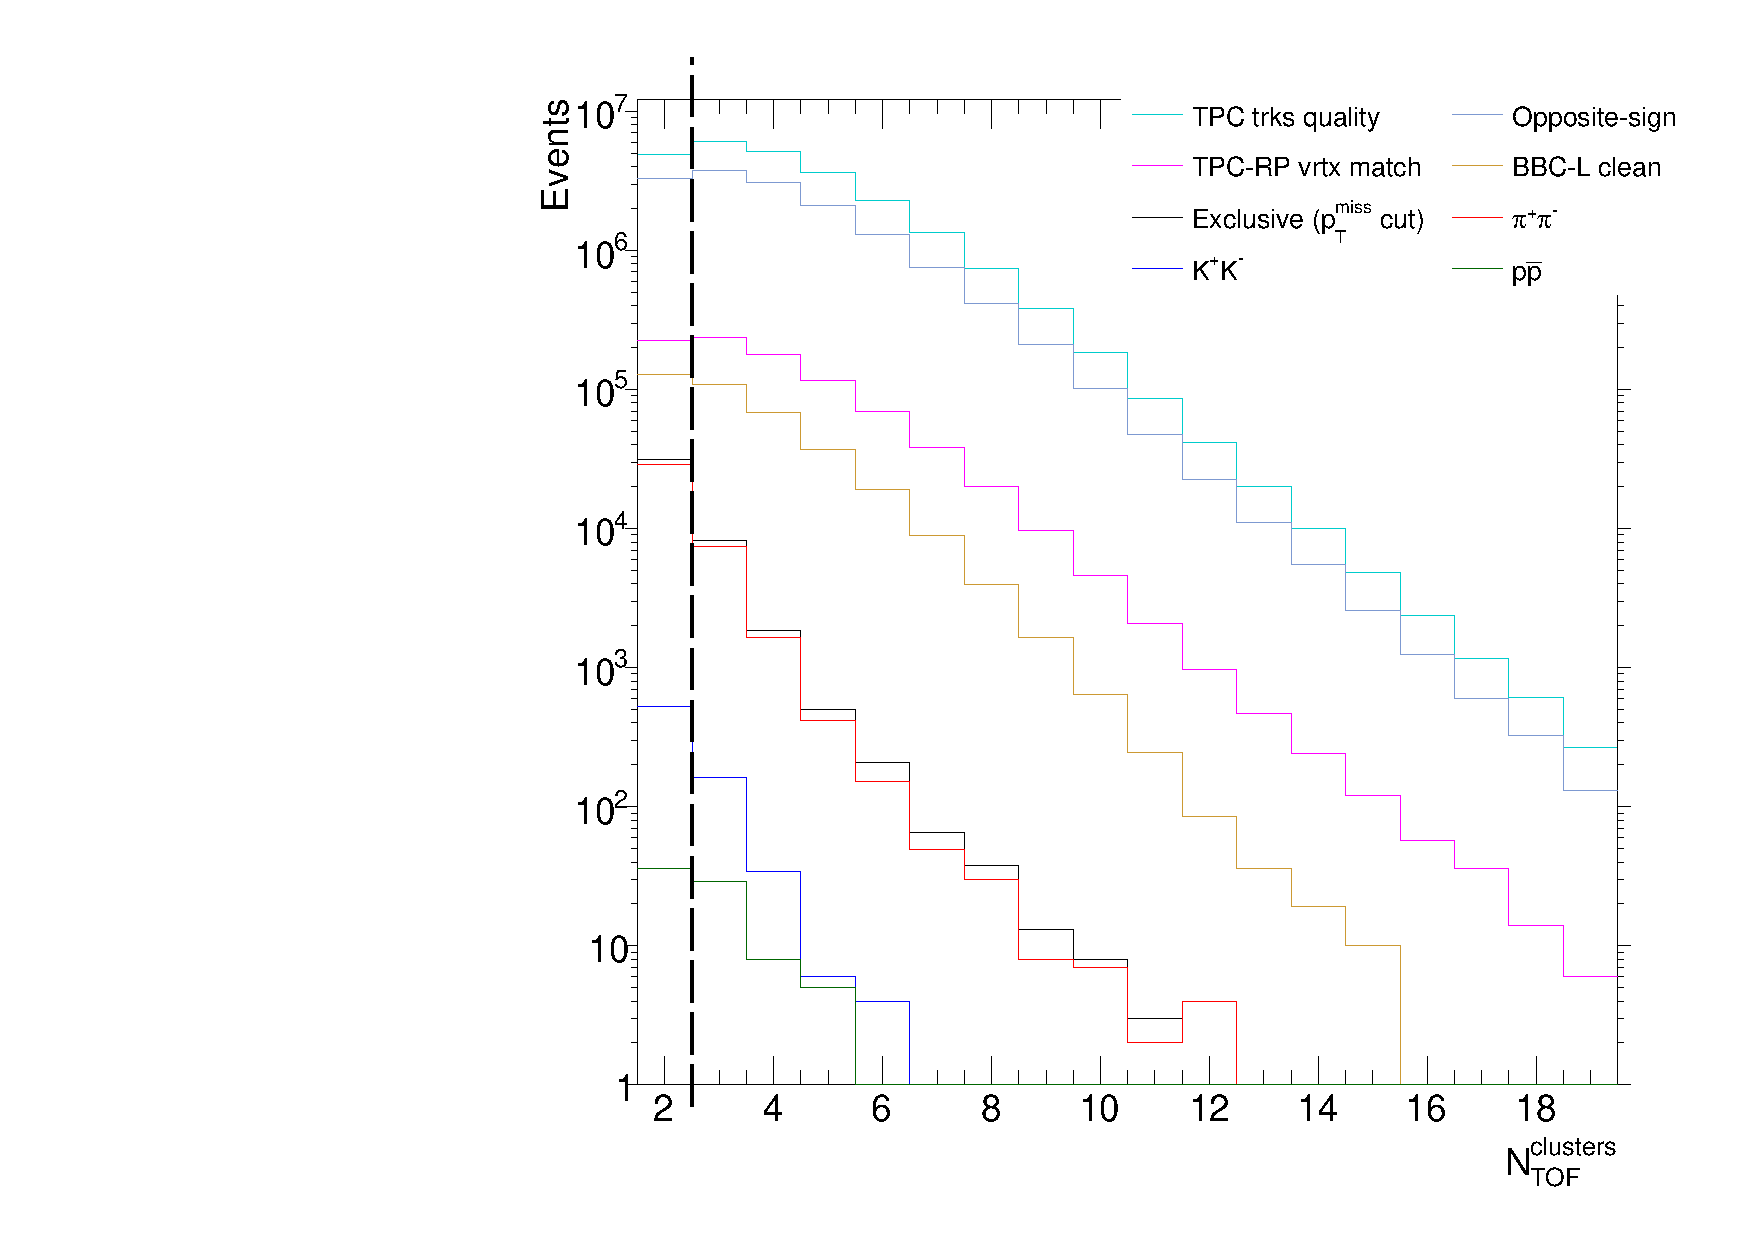
\includegraphics[width=0.475\linewidth,page=1]{graphics/eventSelection/NTofClusters.pdf}%
% % 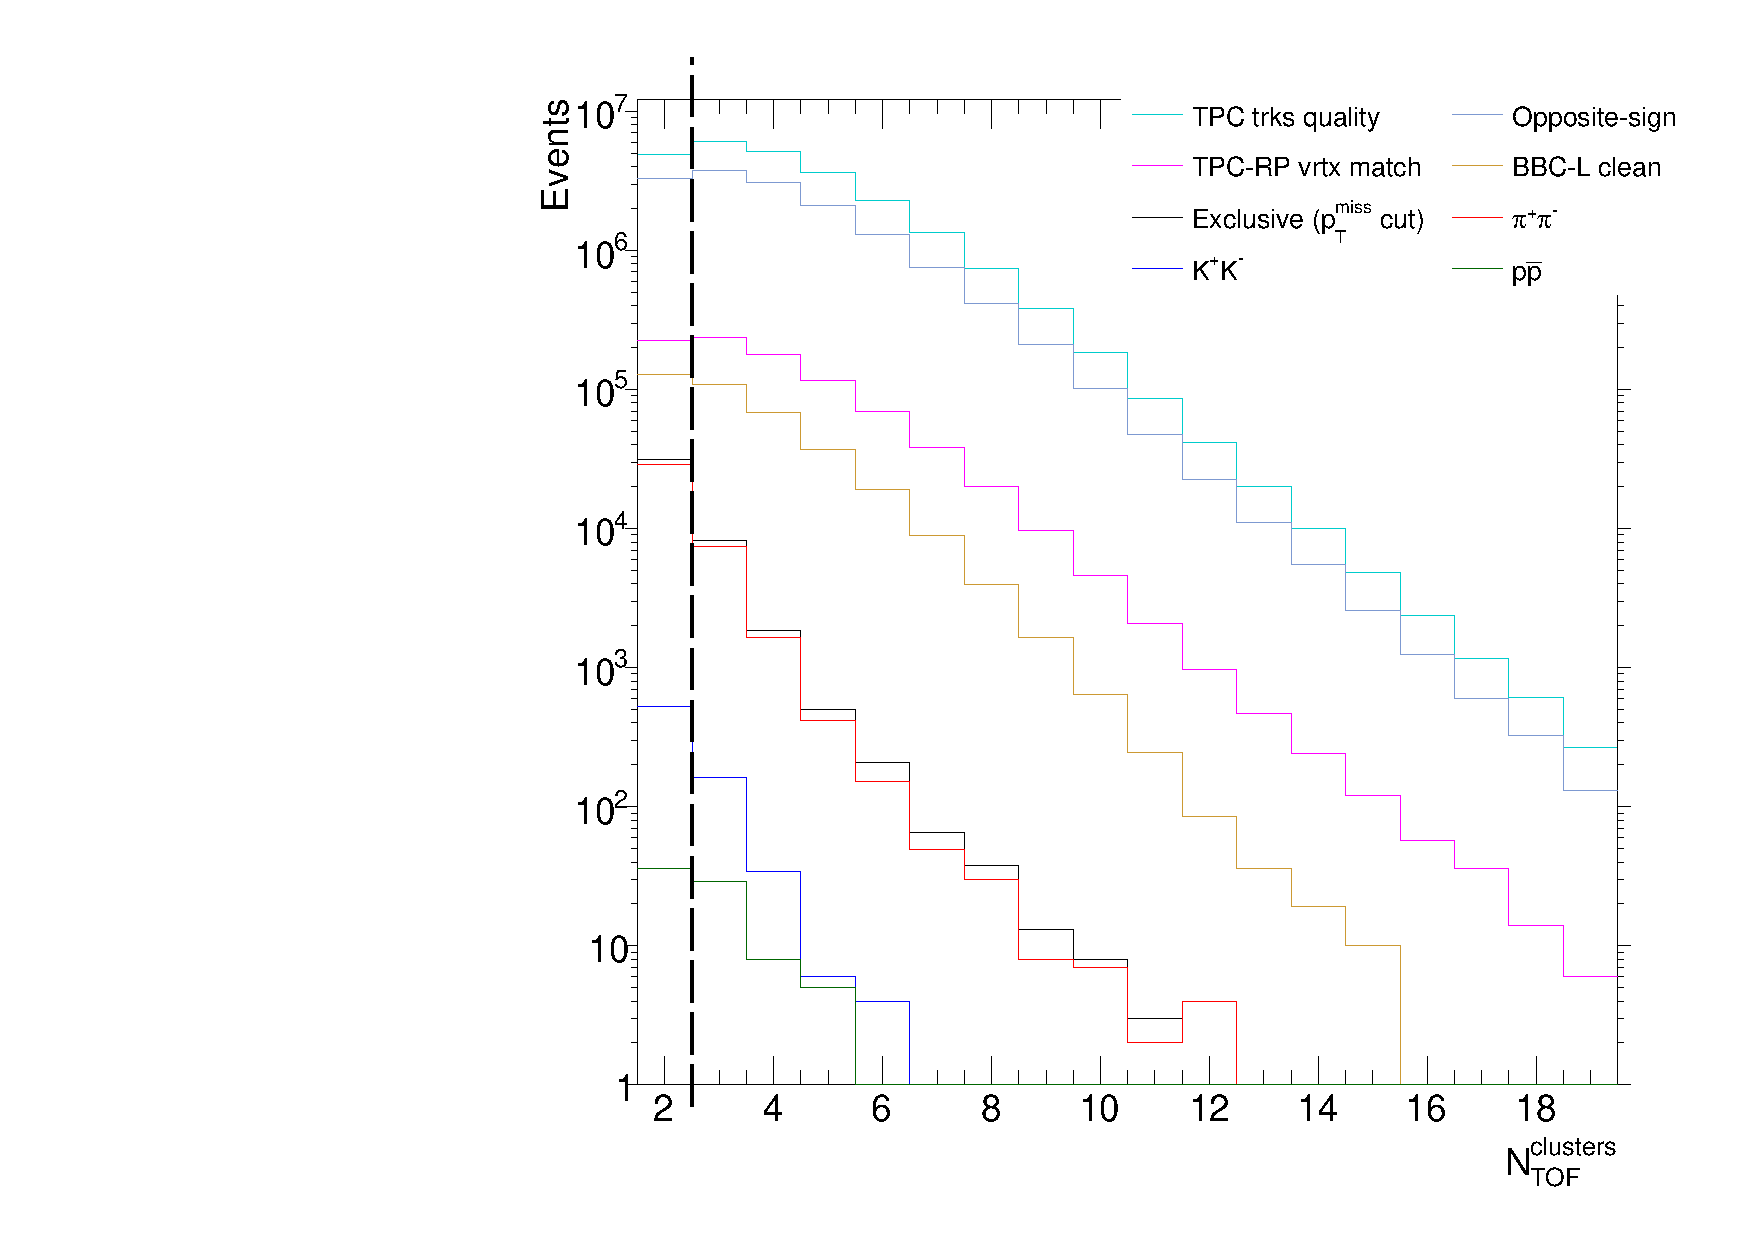
\includegraphics[width=\linewidth,page=1]{graphics/eventSelection/NTofClusters.pdf}%
\caption{NTofClusters.}\label{fig:NTofClusters}%
\end{figure}
% \end{wrapfigure}
%---------------------------

\subsection{(\ref{enum:CutMissingPt})~Exclusivity cut (missing \texorpdfstring{$p_{T}$}{pT} cut)}


%---------------------------
\begin{figure}[ht!]
\centering
\parbox{0.4725\textwidth}{
  \centering
  \begin{subfigure}[b]{\linewidth}{
                \subcaptionbox{\label{fig:PxCentralTrksVsProtons_pion}}{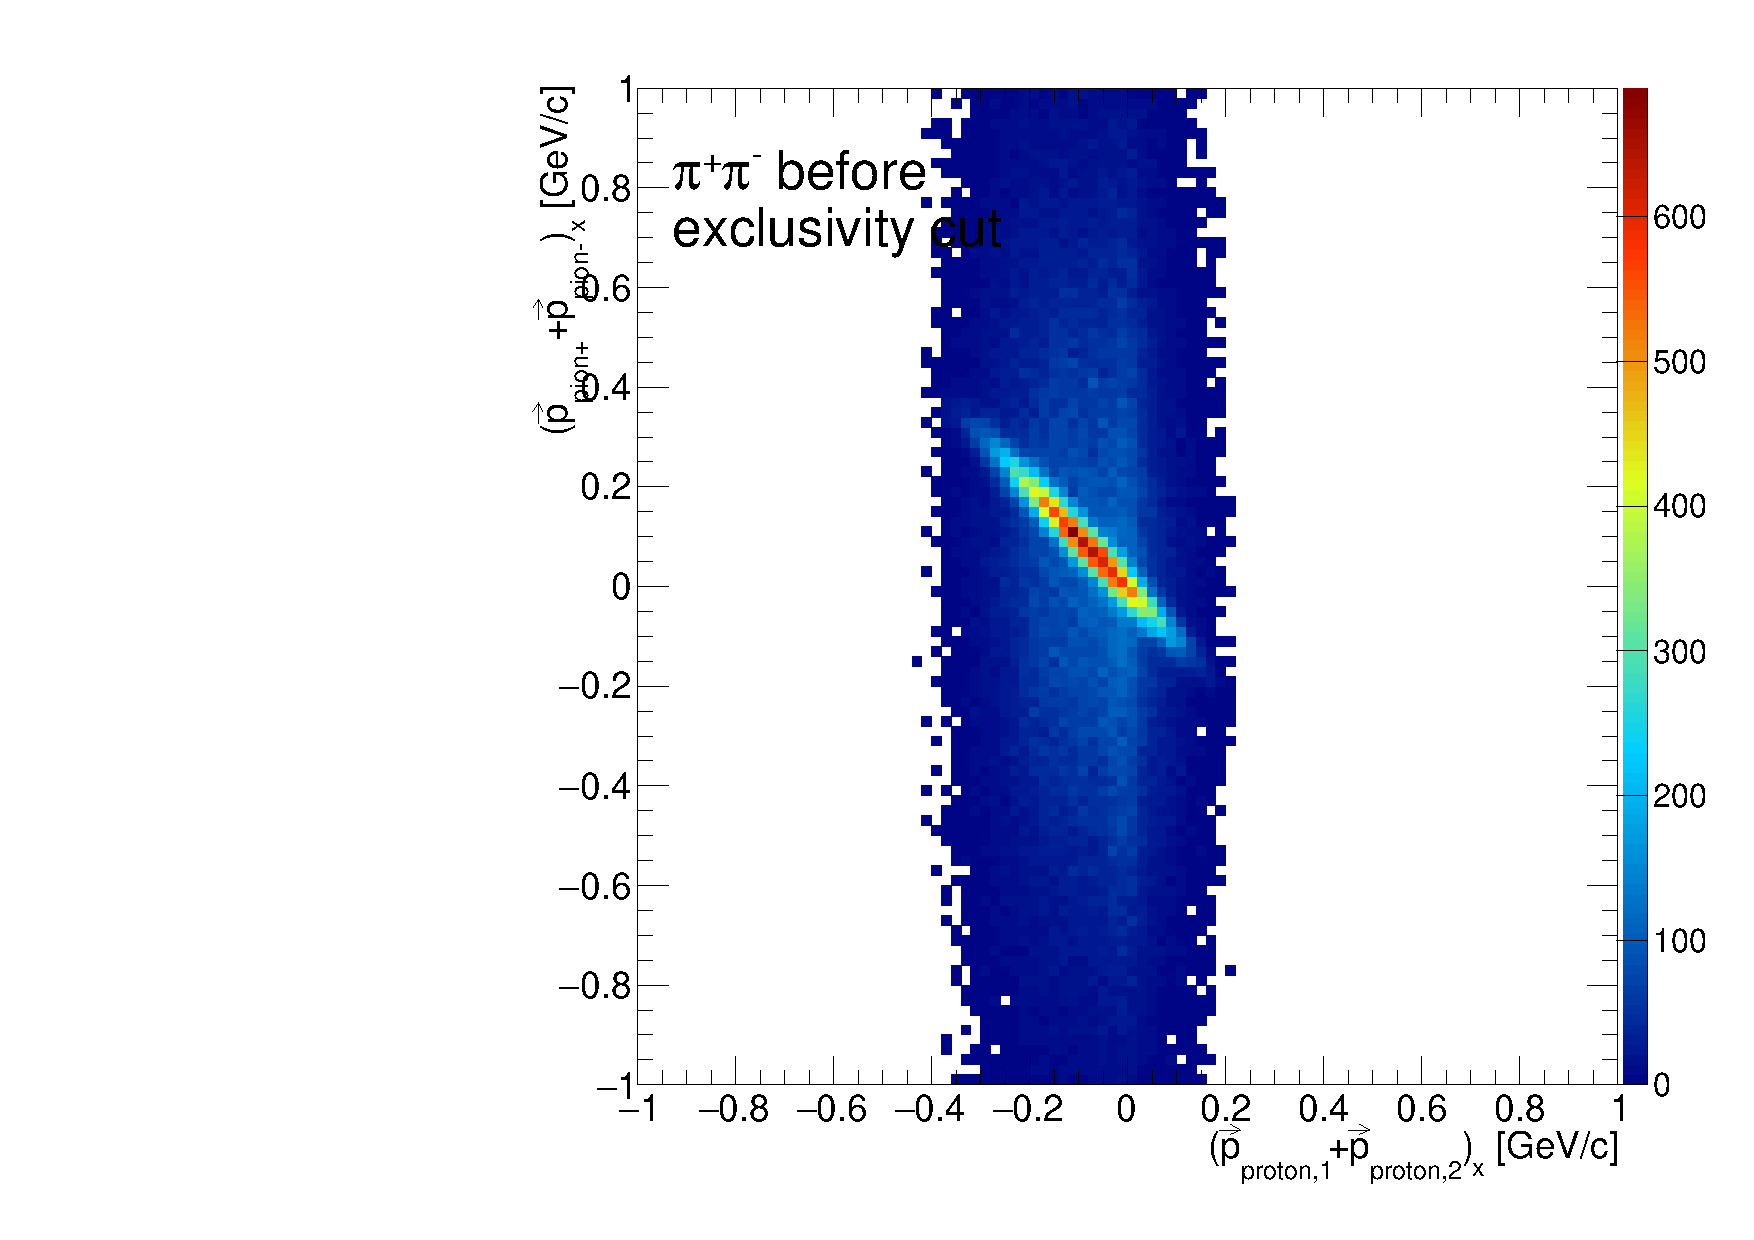
\includegraphics[width=\linewidth]{graphics/eventSelection/PxCentralTrksVsProtons_pion.pdf}}}
  \end{subfigure}
}
\quad
\parbox{0.4725\textwidth}{
  \centering
  \begin{subfigure}[b]{\linewidth}{
                \subcaptionbox{\label{fig:PyCentralTrksVsProtons_pion}}{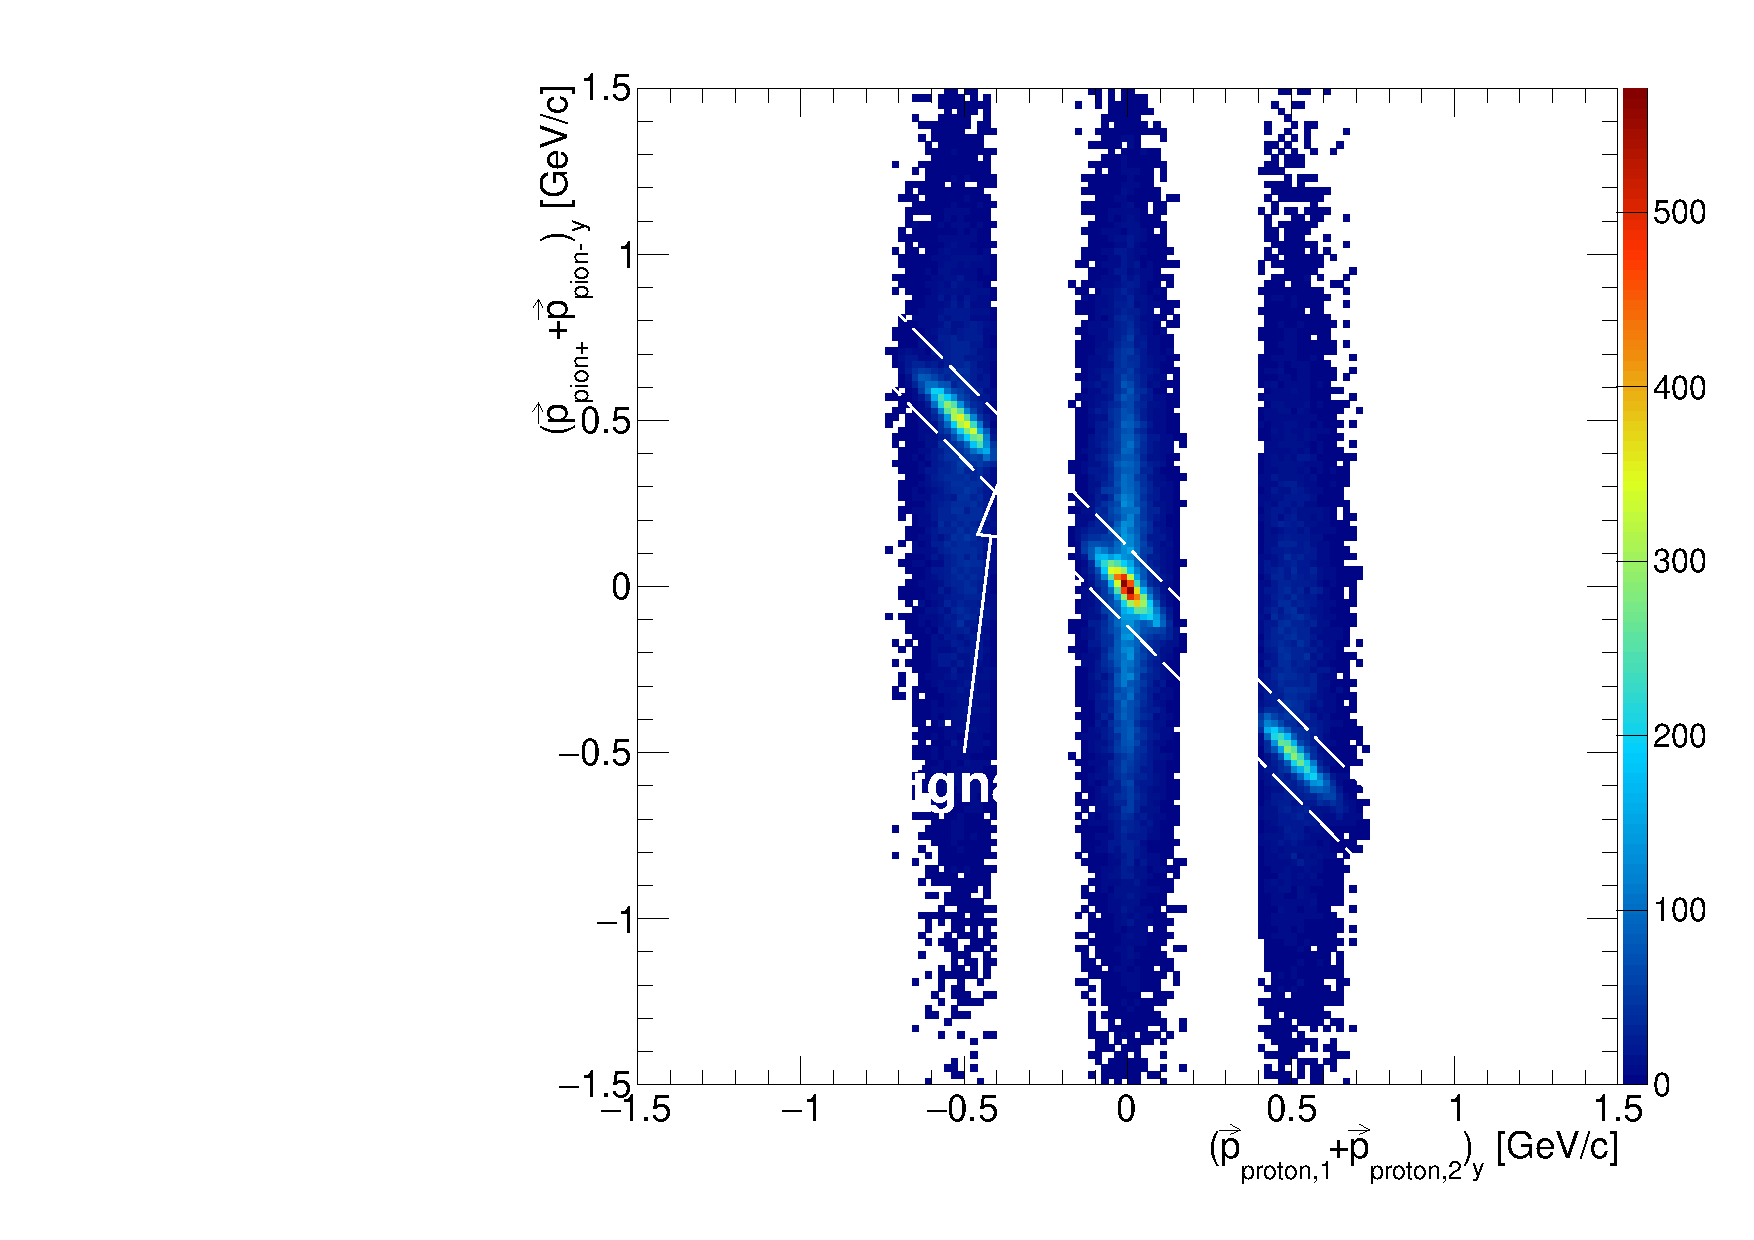
\includegraphics[width=\linewidth]{graphics/eventSelection/PyCentralTrksVsProtons_pion.pdf}}}
  \end{subfigure}
}%
\caption{Correlation between sum of corresponding momentum components ($x$ in Fig.~\ref{fig:PxCentralTrksVsProtons_pion} and $y$ in Fig.~\ref{fig:PyCentralTrksVsProtons_pion}) of Roman Pot proton tracks and TPC tracks.}
\end{figure}
Tutaj dodac rysunki z suma 1D tych wielkosci i uzasadnic stosowanie ciecia na missing pT takimi samymi rozdzielczosciami w x i y
%---------------------------


%---------------------------
\begin{figure}[ht!]
% \begin{wrapfigure}{l}{0.475\textwidth}%[ht!]
\centering%
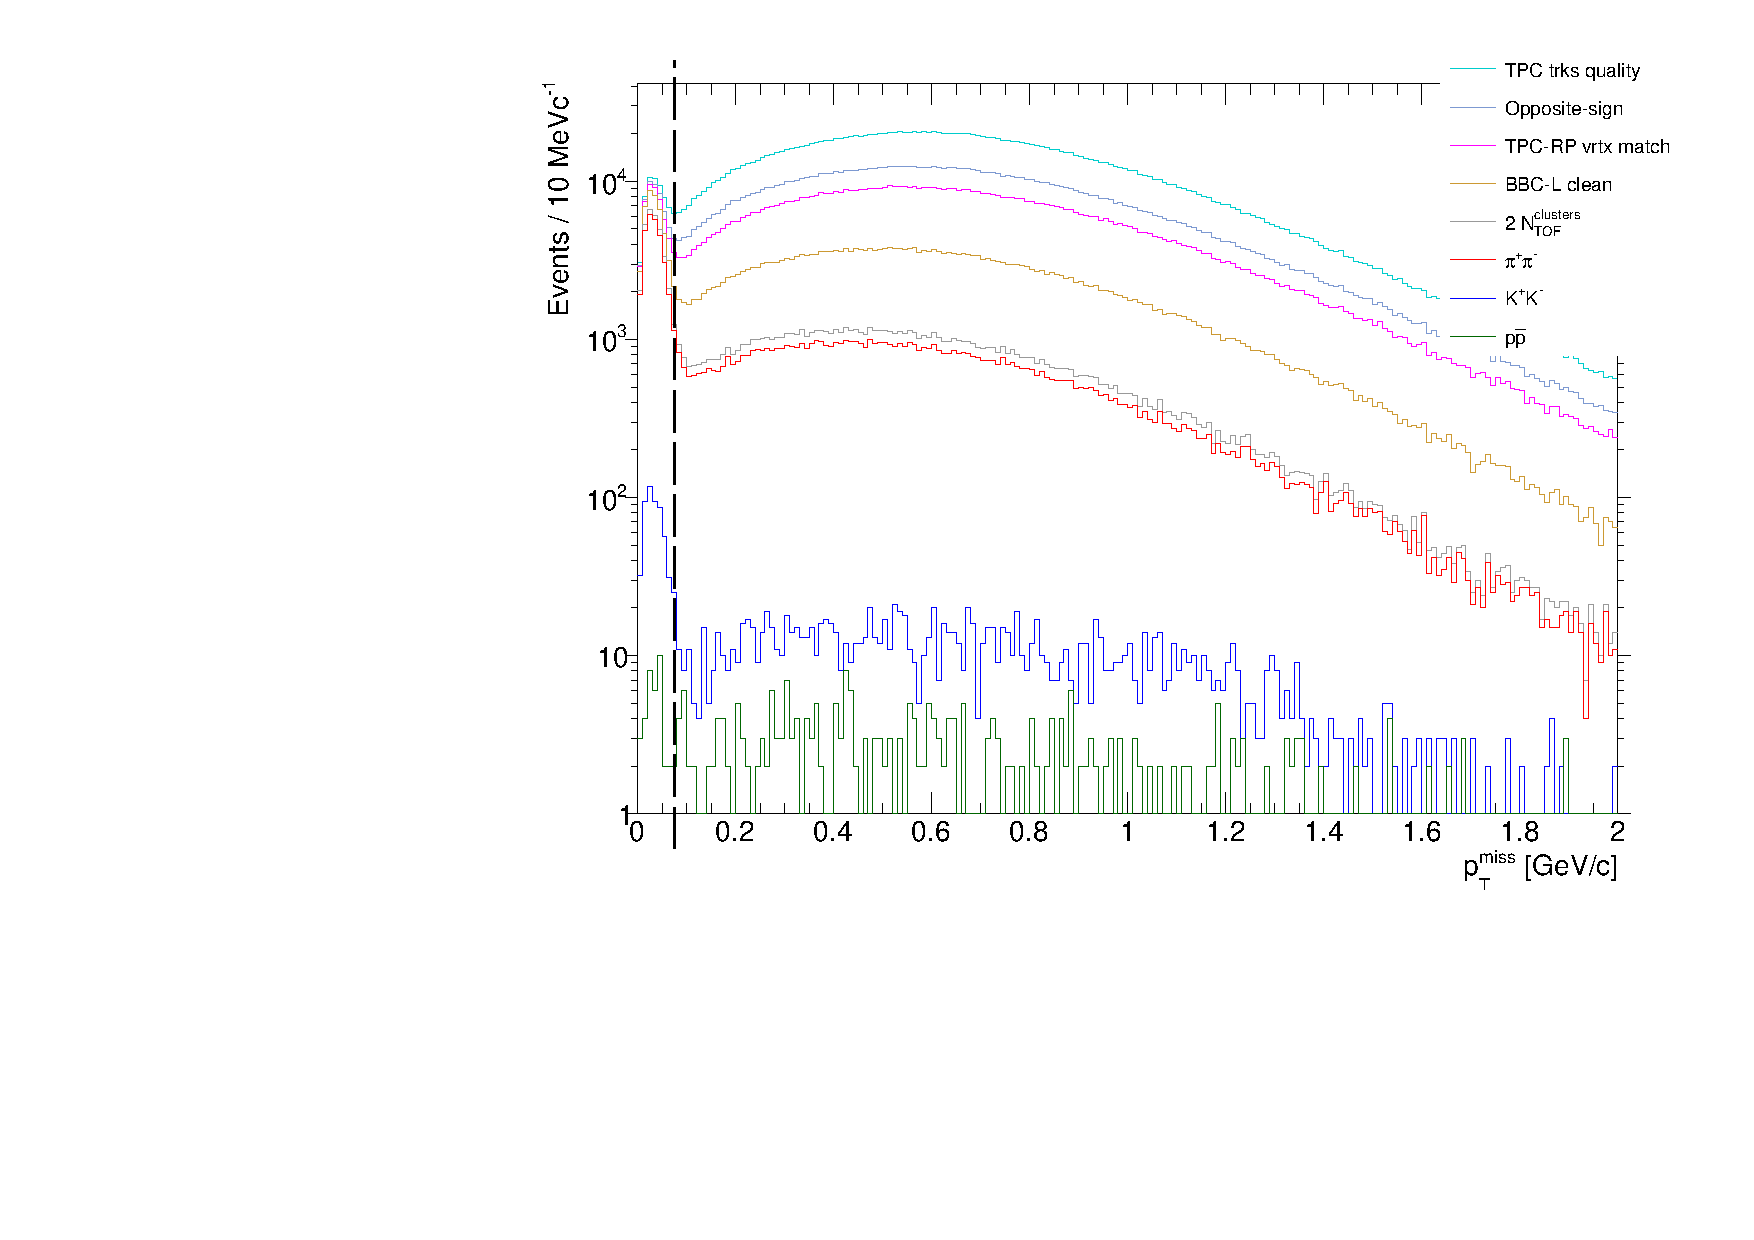
\includegraphics[width=0.633\linewidth,page=1]{graphics/eventSelection/MissingPt.pdf}%
% % 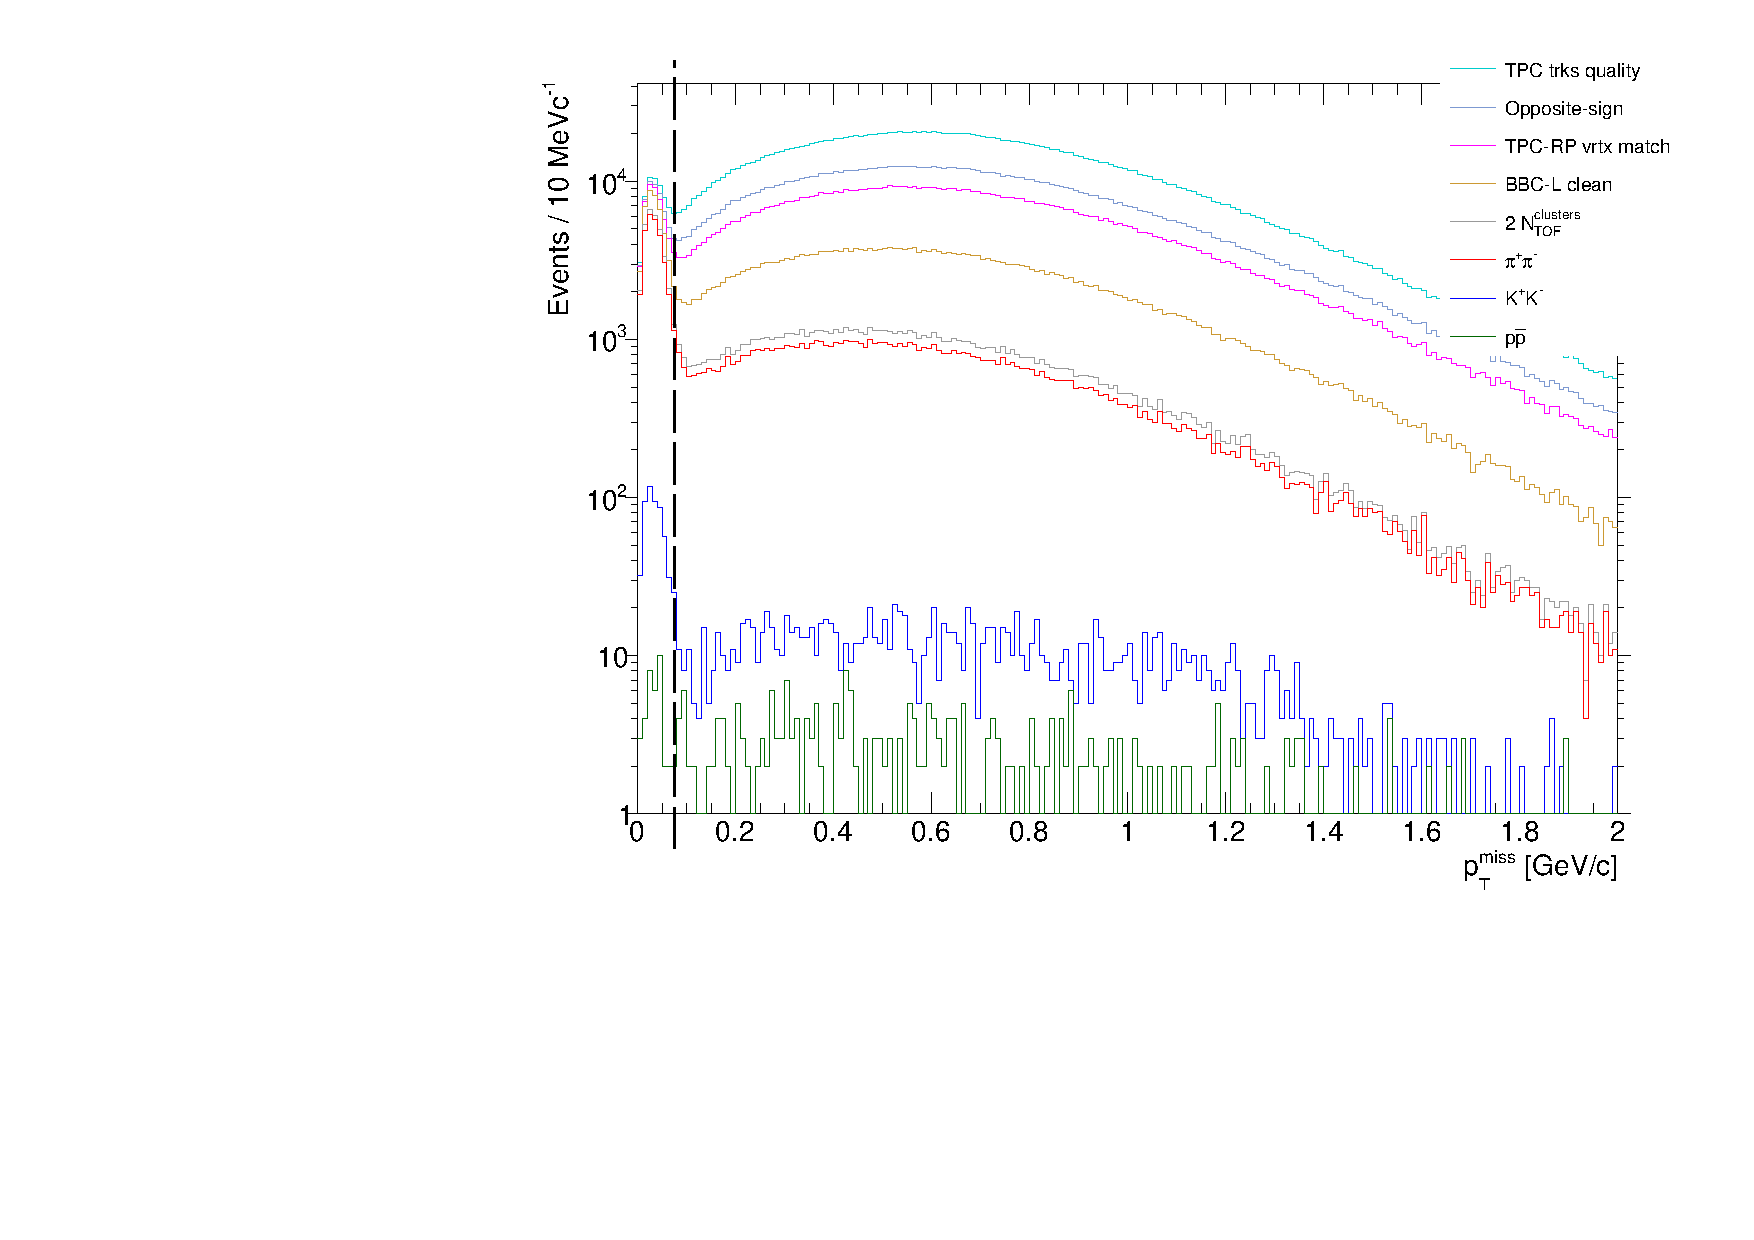
\includegraphics[width=\linewidth,page=1]{graphics/eventSelection/MissingPt.pdf}%
\caption{MissingPt.}\label{fig:MissingPt}%
\end{figure}
% \end{wrapfigure}
%---------------------------


\subsection{(\ref{enum:CutPid})~Particle identification}

In addition to information from the TPC we use time of hit detection in the barrel TOF subsystem. 






%---------------------------
\begin{figure}[ht!]
\centering
\parbox{0.315\textwidth}{
  \centering
  \begin{subfigure}[b]{\linewidth}{
                \subcaptionbox{\label{fig:SqRootNSigmaPionVsKaon}}{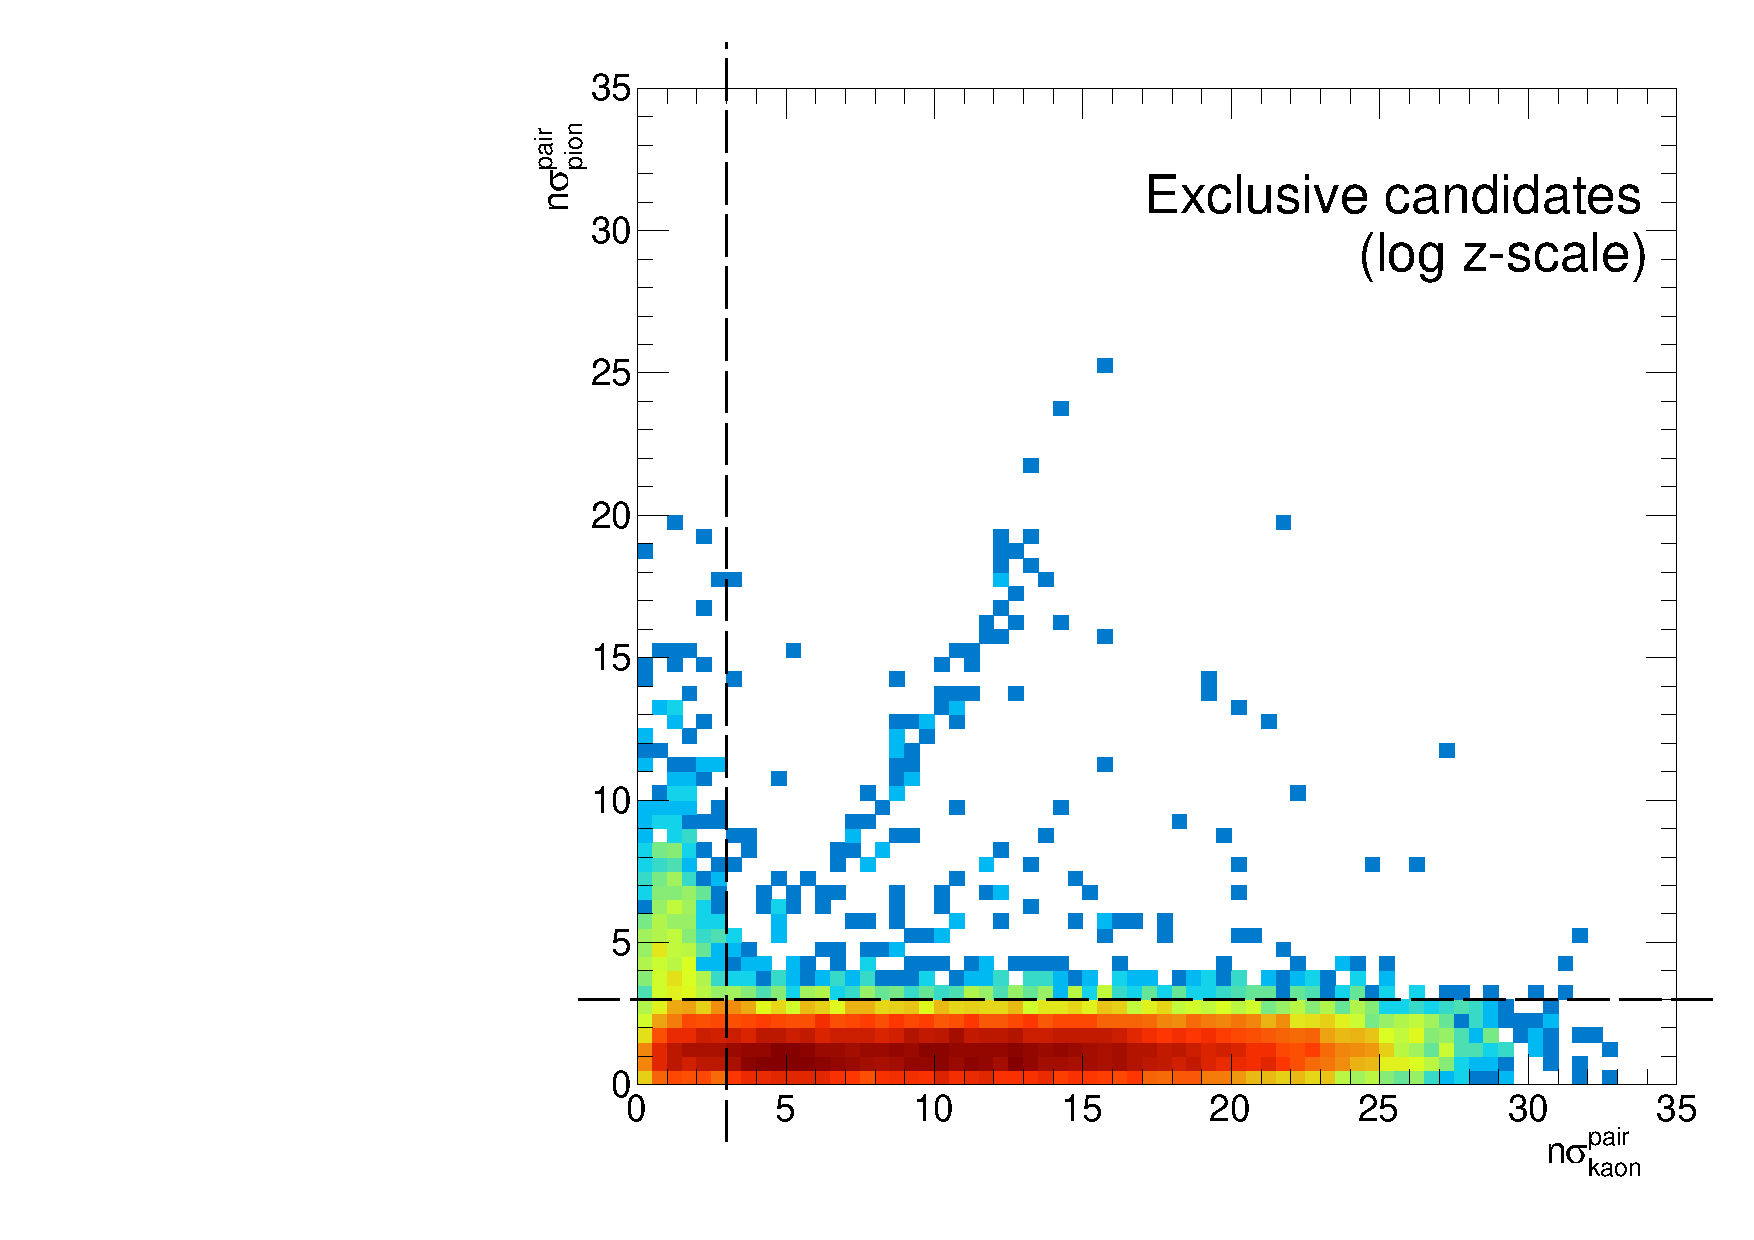
\includegraphics[width=\linewidth]{graphics/eventSelection/SqRootNSigmaPionVsKaon.pdf}}}
  \end{subfigure}
}
\quad
\parbox{0.315\textwidth}{
  \centering
  \begin{subfigure}[b]{\linewidth}{
                \subcaptionbox{\label{fig:SqRootNSigmaPionVsProton}}{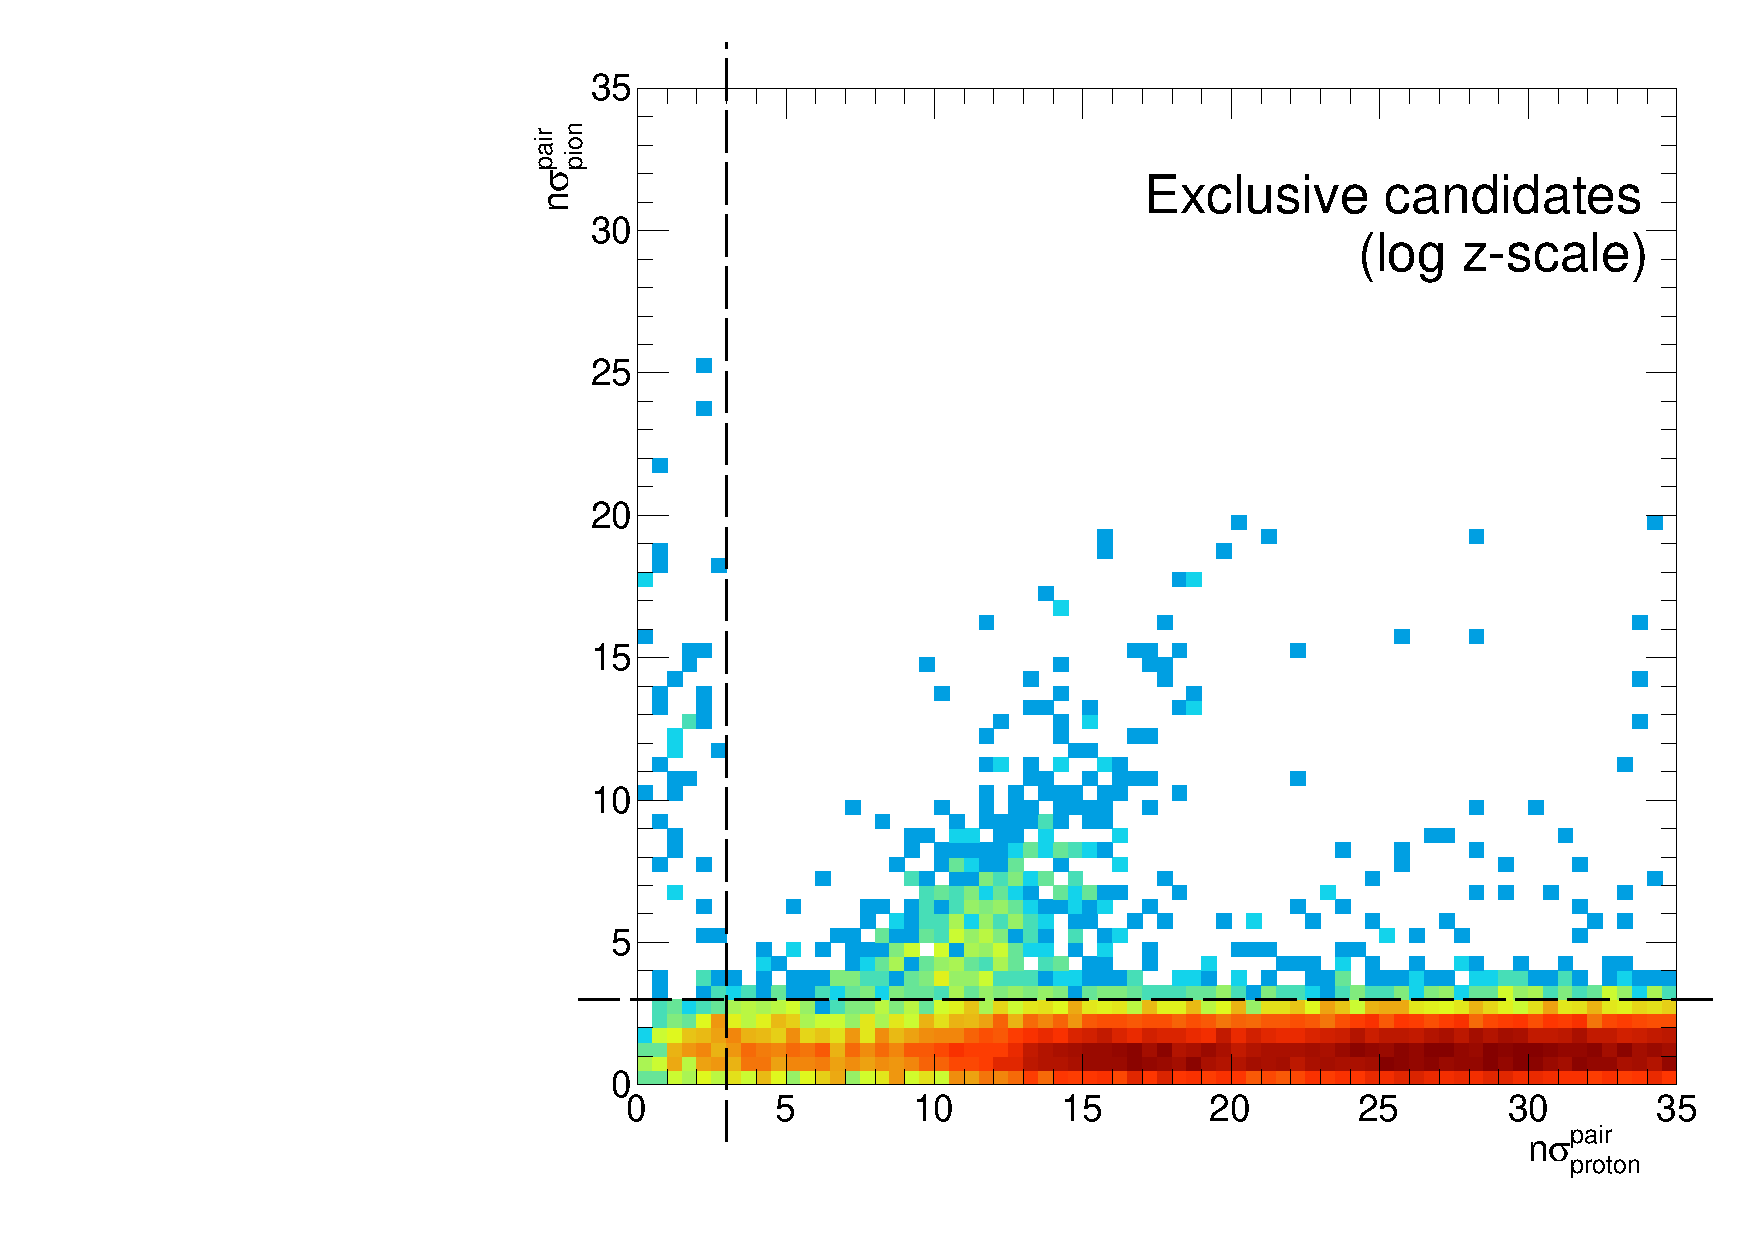
\includegraphics[width=\linewidth]{graphics/eventSelection/SqRootNSigmaPionVsProton.pdf}}}
  \end{subfigure}
}
\quad
\parbox{0.315\textwidth}{
  \centering
  \begin{subfigure}[b]{\linewidth}{
                \subcaptionbox{\label{fig:SqRootNSigmaKaonVsProton}}{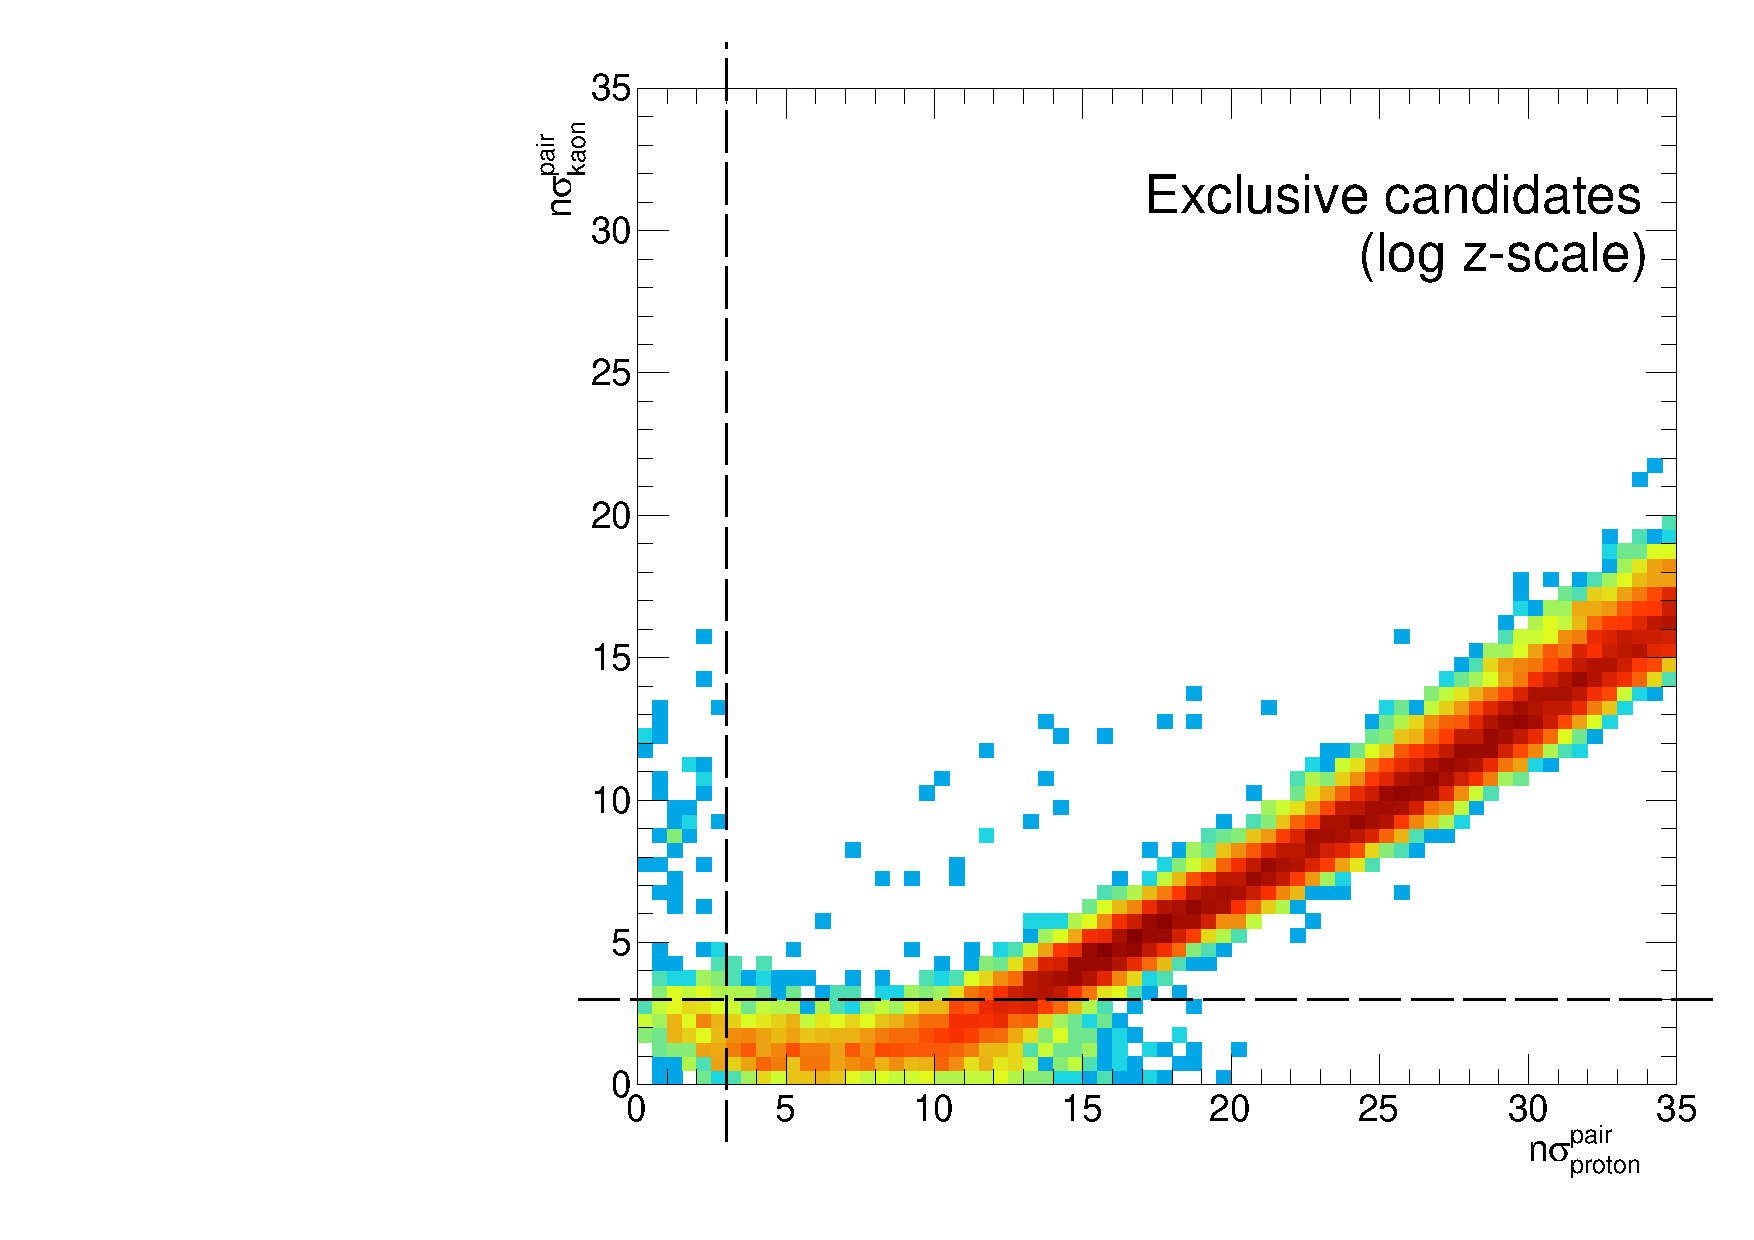
\includegraphics[width=\linewidth]{graphics/eventSelection/SqRootNSigmaKaonVsProton.pdf}}}
  \end{subfigure}
}%
\caption{Correlation between $n\sigma^{\text{pair}}$ from TPC for $\pi^{+}\pi^{-}$, $K^{+}K^{-}$ and $p\bar{p}$.}
\end{figure}
%---------------------------


%---------------------------
\begin{figure}[ht!]
\centering
\parbox{0.315\textwidth}{
  \centering
  \begin{subfigure}[b]{\linewidth}{
                \subcaptionbox{\label{fig:SqMassTofVsSqRootNSigma_pion}}{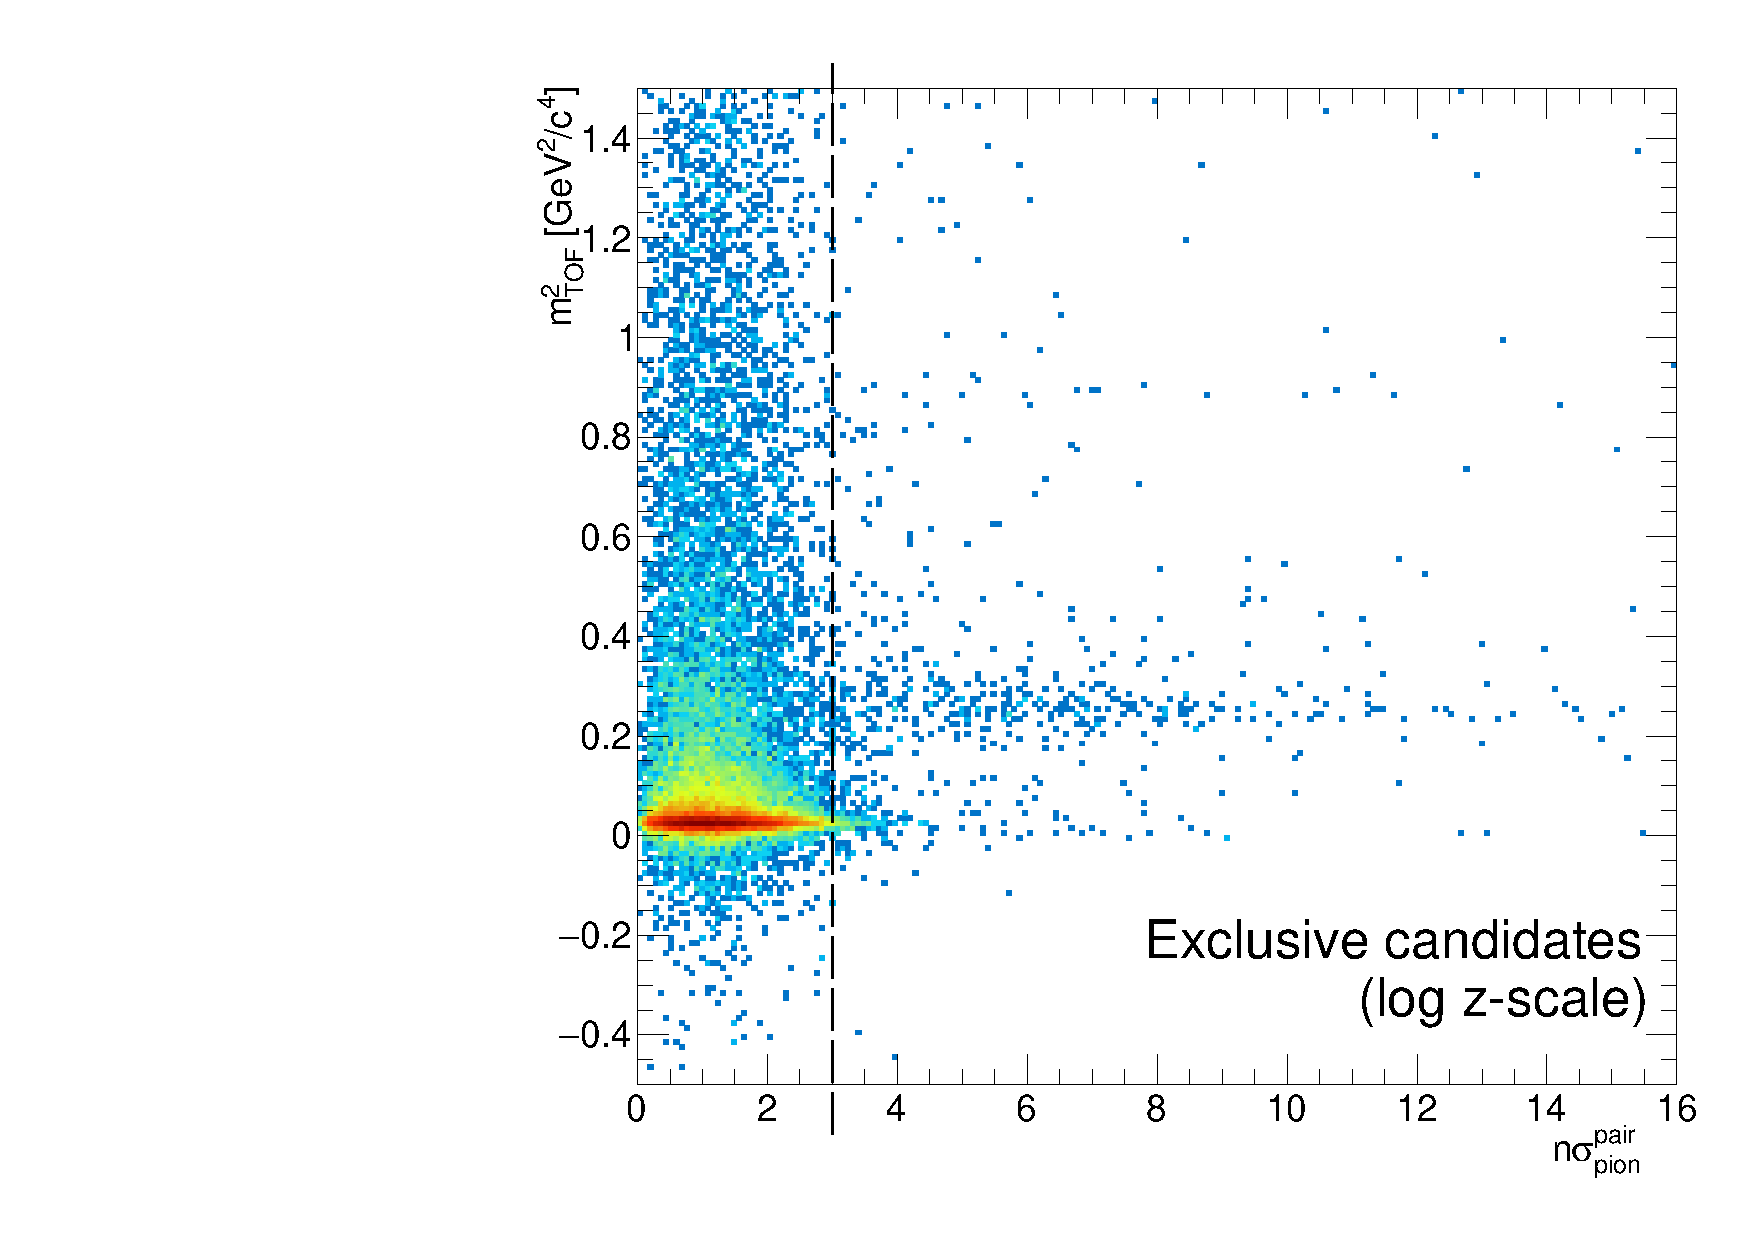
\includegraphics[width=\linewidth]{graphics/eventSelection/SqMassTofVsSqRootNSigma_pion.pdf}}}
  \end{subfigure}
}
\quad
\parbox{0.315\textwidth}{
  \centering
  \begin{subfigure}[b]{\linewidth}{
                \subcaptionbox{\label{fig:SqMassTofVsSqRootNSigma_kaon}}{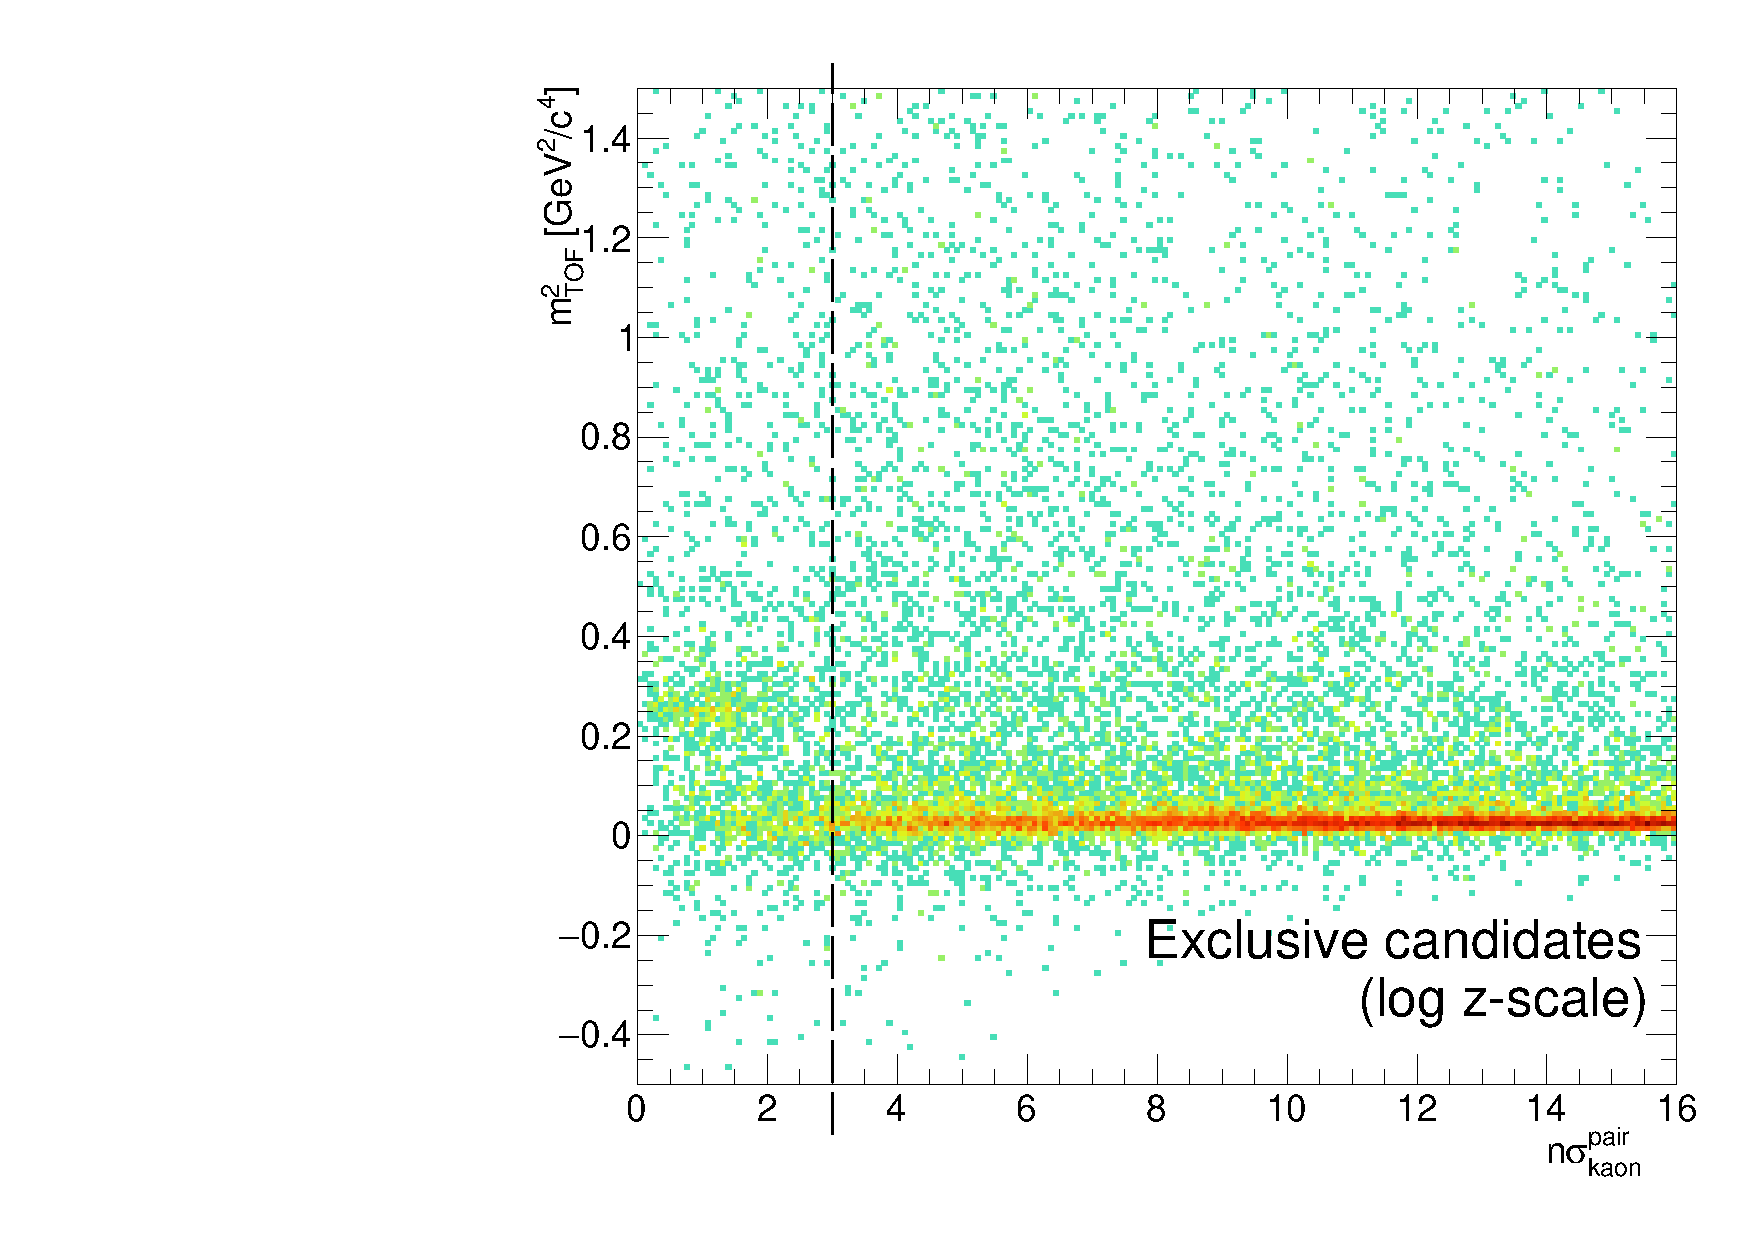
\includegraphics[width=\linewidth]{graphics/eventSelection/SqMassTofVsSqRootNSigma_kaon.pdf}}}
  \end{subfigure}
}
\quad
\parbox{0.315\textwidth}{
  \centering
  \begin{subfigure}[b]{\linewidth}{
                \subcaptionbox{\label{fig:SqMassTofVsSqRootNSigma_proton}}{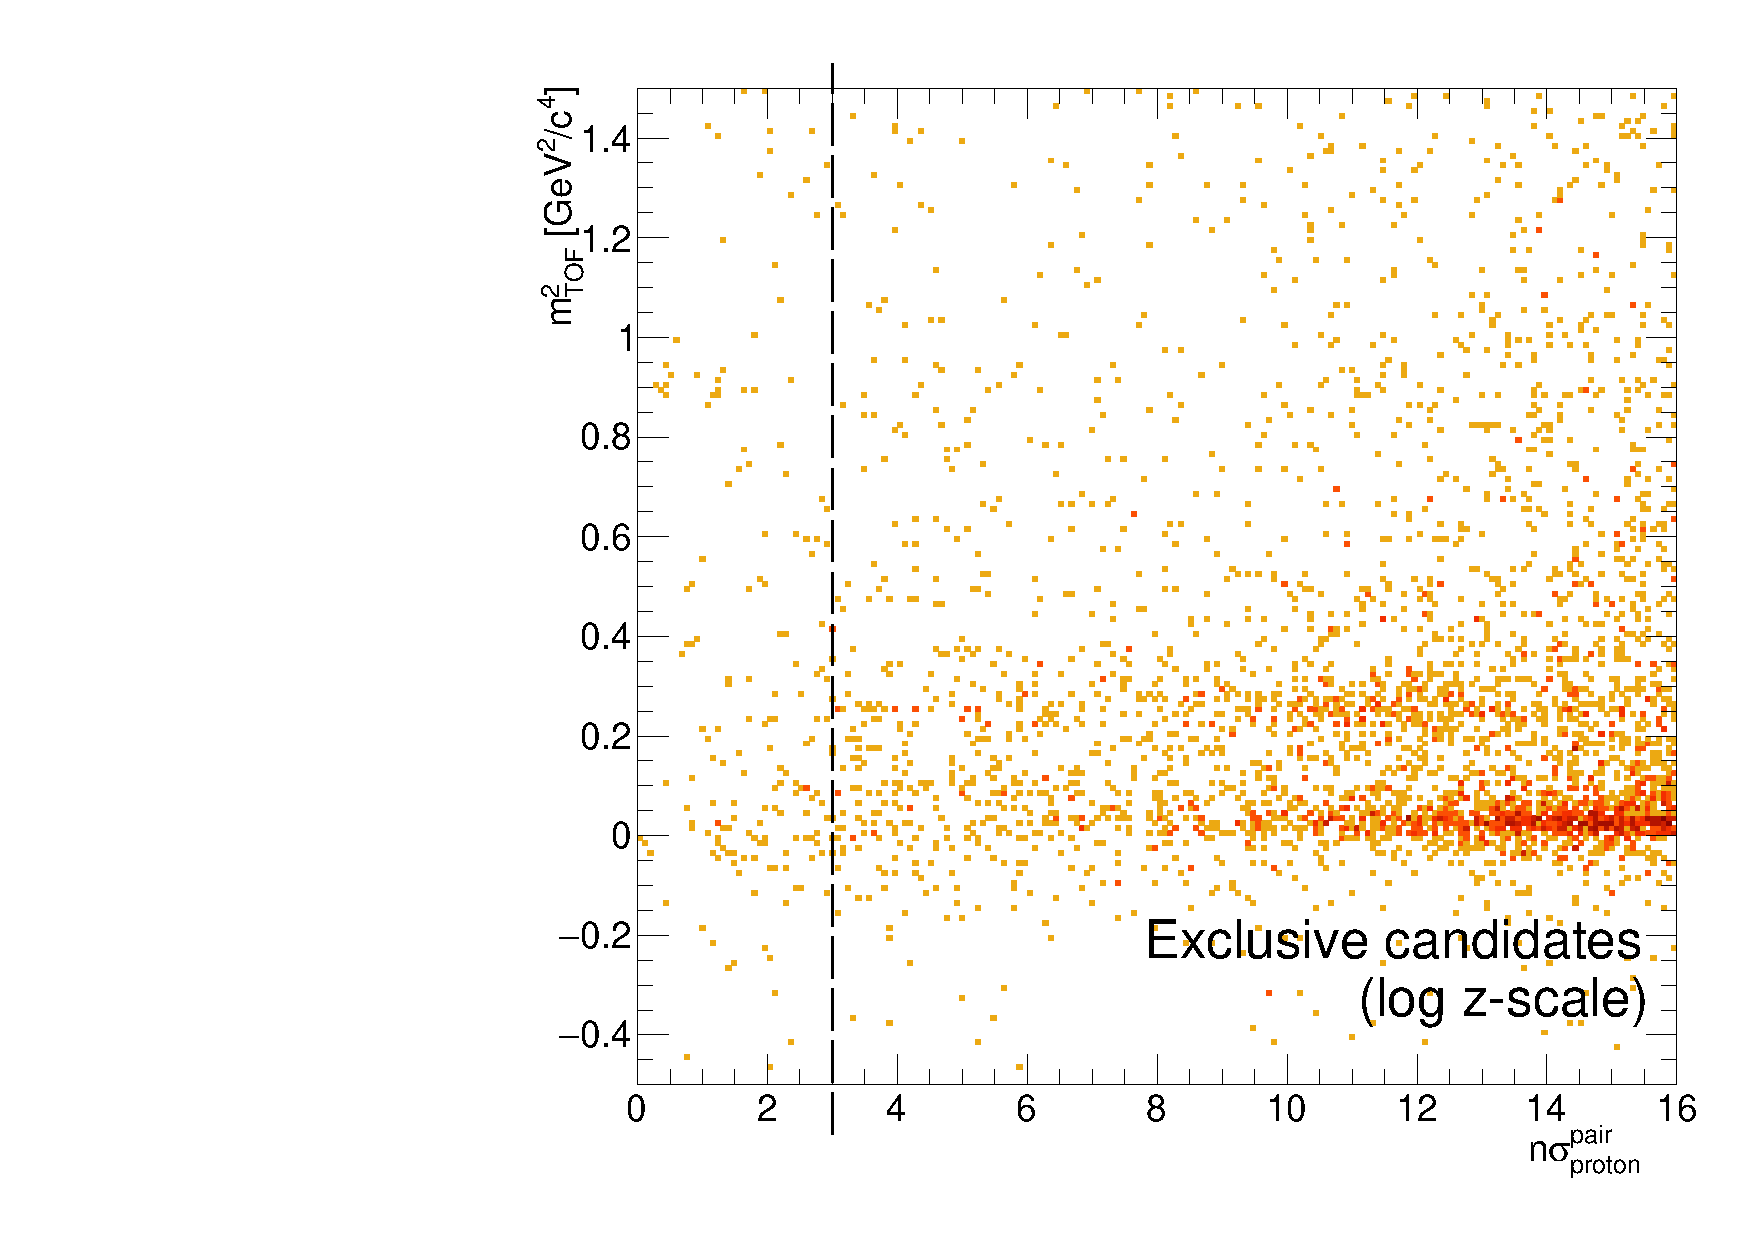
\includegraphics[width=\linewidth]{graphics/eventSelection/SqMassTofVsSqRootNSigma_proton.pdf}}}
  \end{subfigure}
}%
\caption{Correlation between $m^{2}$ from TOF and $n\sigma^{\text{pair}}$ from TPC for $\pi^{+}\pi^{-}$, $K^{+}K^{-}$ and $p\bar{p}$.}
\end{figure}
%---------------------------







%---------------------------
\begin{figure}[ht!]
\centering%
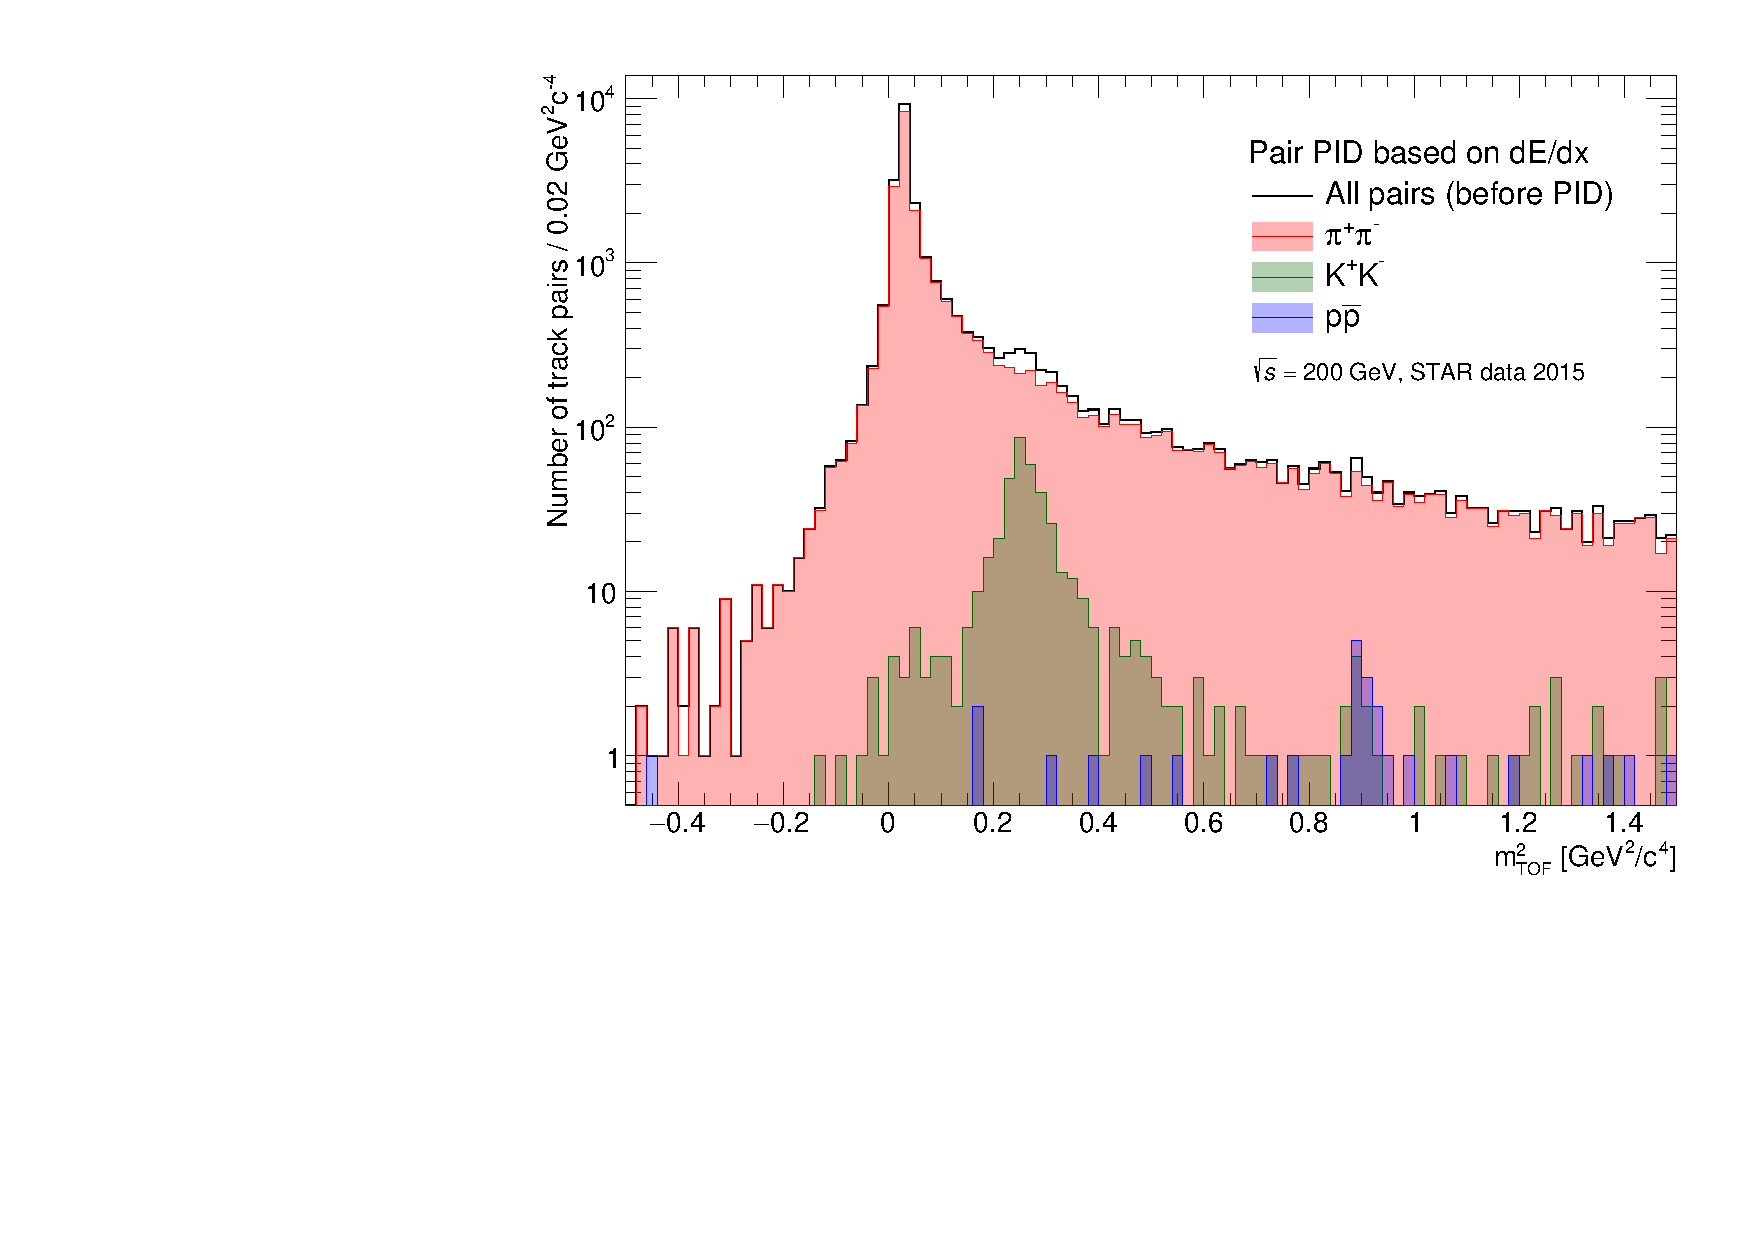
\includegraphics[width=0.65\linewidth,page=1]{graphics/eventSelection/sqMassFromTof.pdf}%
\caption{Squared particle mass from TOF for candidates of given PID selected based on $dE/dx$ in TPC.}\label{fig:sqMassFromTof}%
\end{figure}
%---------------------------









\section{Working point for cuts~\ref{enum:CutBbcLarge}, \ref{enum:CutTofClusters} and \ref{enum:CutMissingPt}}

\begin{tabulary}{\textwidth}{LLL}
\begin{equation}\label{eq:significance}\hspace*{-10pt}
	\text{Significance} = \frac{N_{\text{signal}}^{\text{cut}}}{\sqrt{N_{\text{signal}}^{\text{cut}} + N_{\text{bkgd}}^{\text{cut}}}},
\end{equation}~~~~~~~~~~~~~~~~~&
\begin{equation}\label{eq:efficiency}\hspace*{-10pt}
	\text{Efficiency} = \frac{N_{\text{signal}}^{\text{cut}}}{N_{\text{signal}}^{\text{no~cut}}},
\end{equation}~~~~~~~~~~~~~~&
\begin{equation}\label{eq:purity}\hspace*{-9pt}
	\text{Purity} = \frac{N_{\text{signal}}^{\text{cut}}}{N_{\text{signal}}^{\text{cut}}+N_{\text{bkgd}}^{\text{cut}}},
\end{equation}~~~~~~~~~~~~~~~
\end{tabulary}


%---------------------------
\begin{figure}[hb]
\centering
\parbox{0.4725\textwidth}{
  \centering
  \begin{subfigure}[b]{\linewidth}
                \subcaptionbox{\label{fig:SignificanceVsEff}}{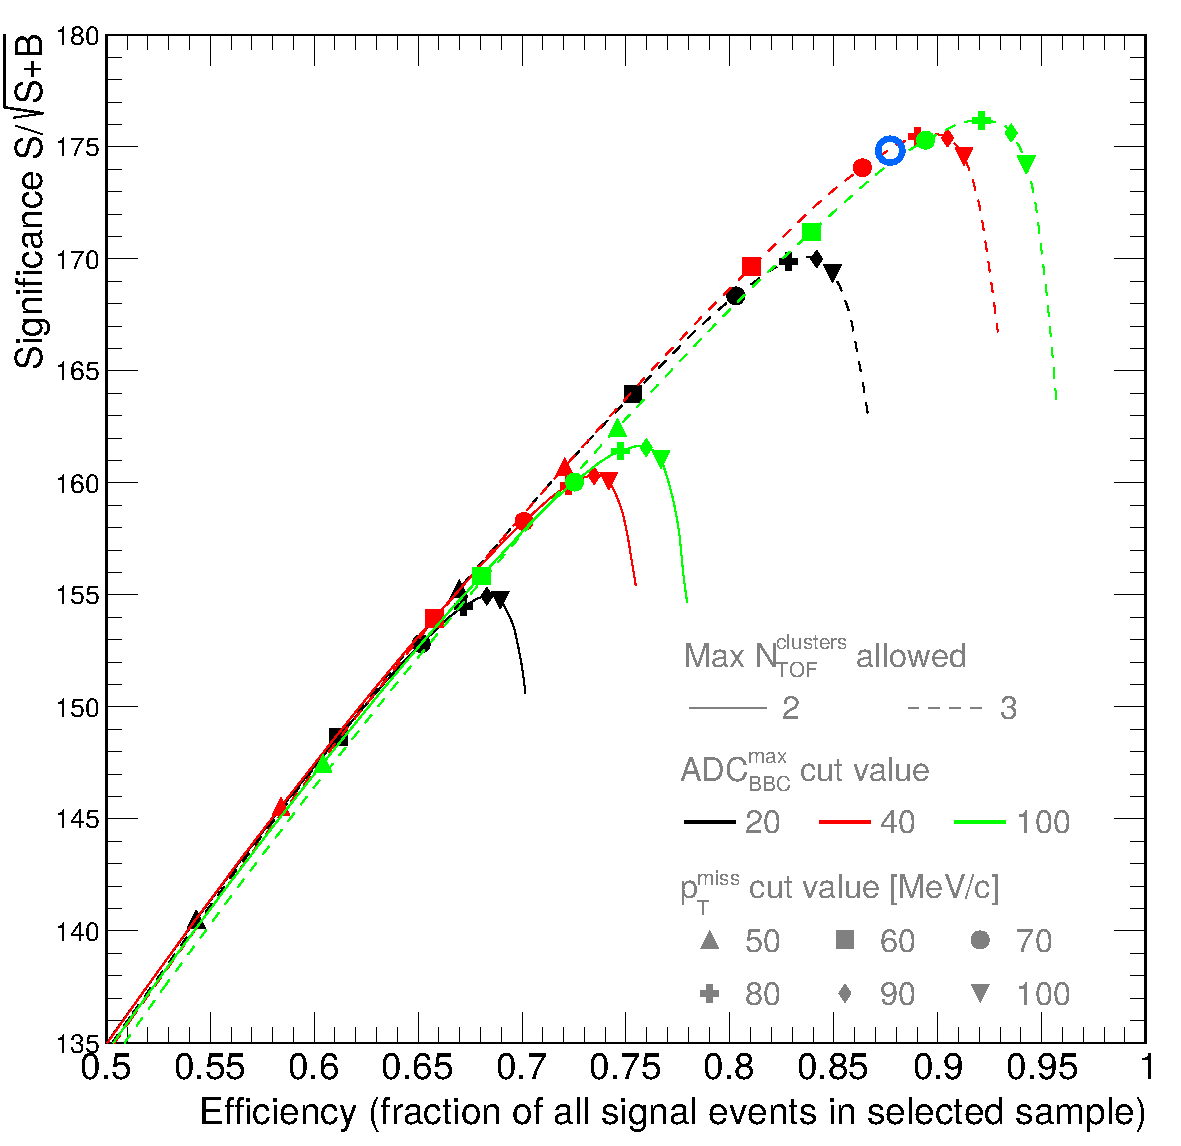
\includegraphics[width=\linewidth]{graphics/eventSelection/SignificanceVsEfficiency_pTmiss.pdf}}
  \end{subfigure}\\
  \begin{subfigure}[b]{\linewidth}\addtocounter{subfigure}{1}
                \subcaptionbox{\label{fig:EffVsBkgdFrac}}{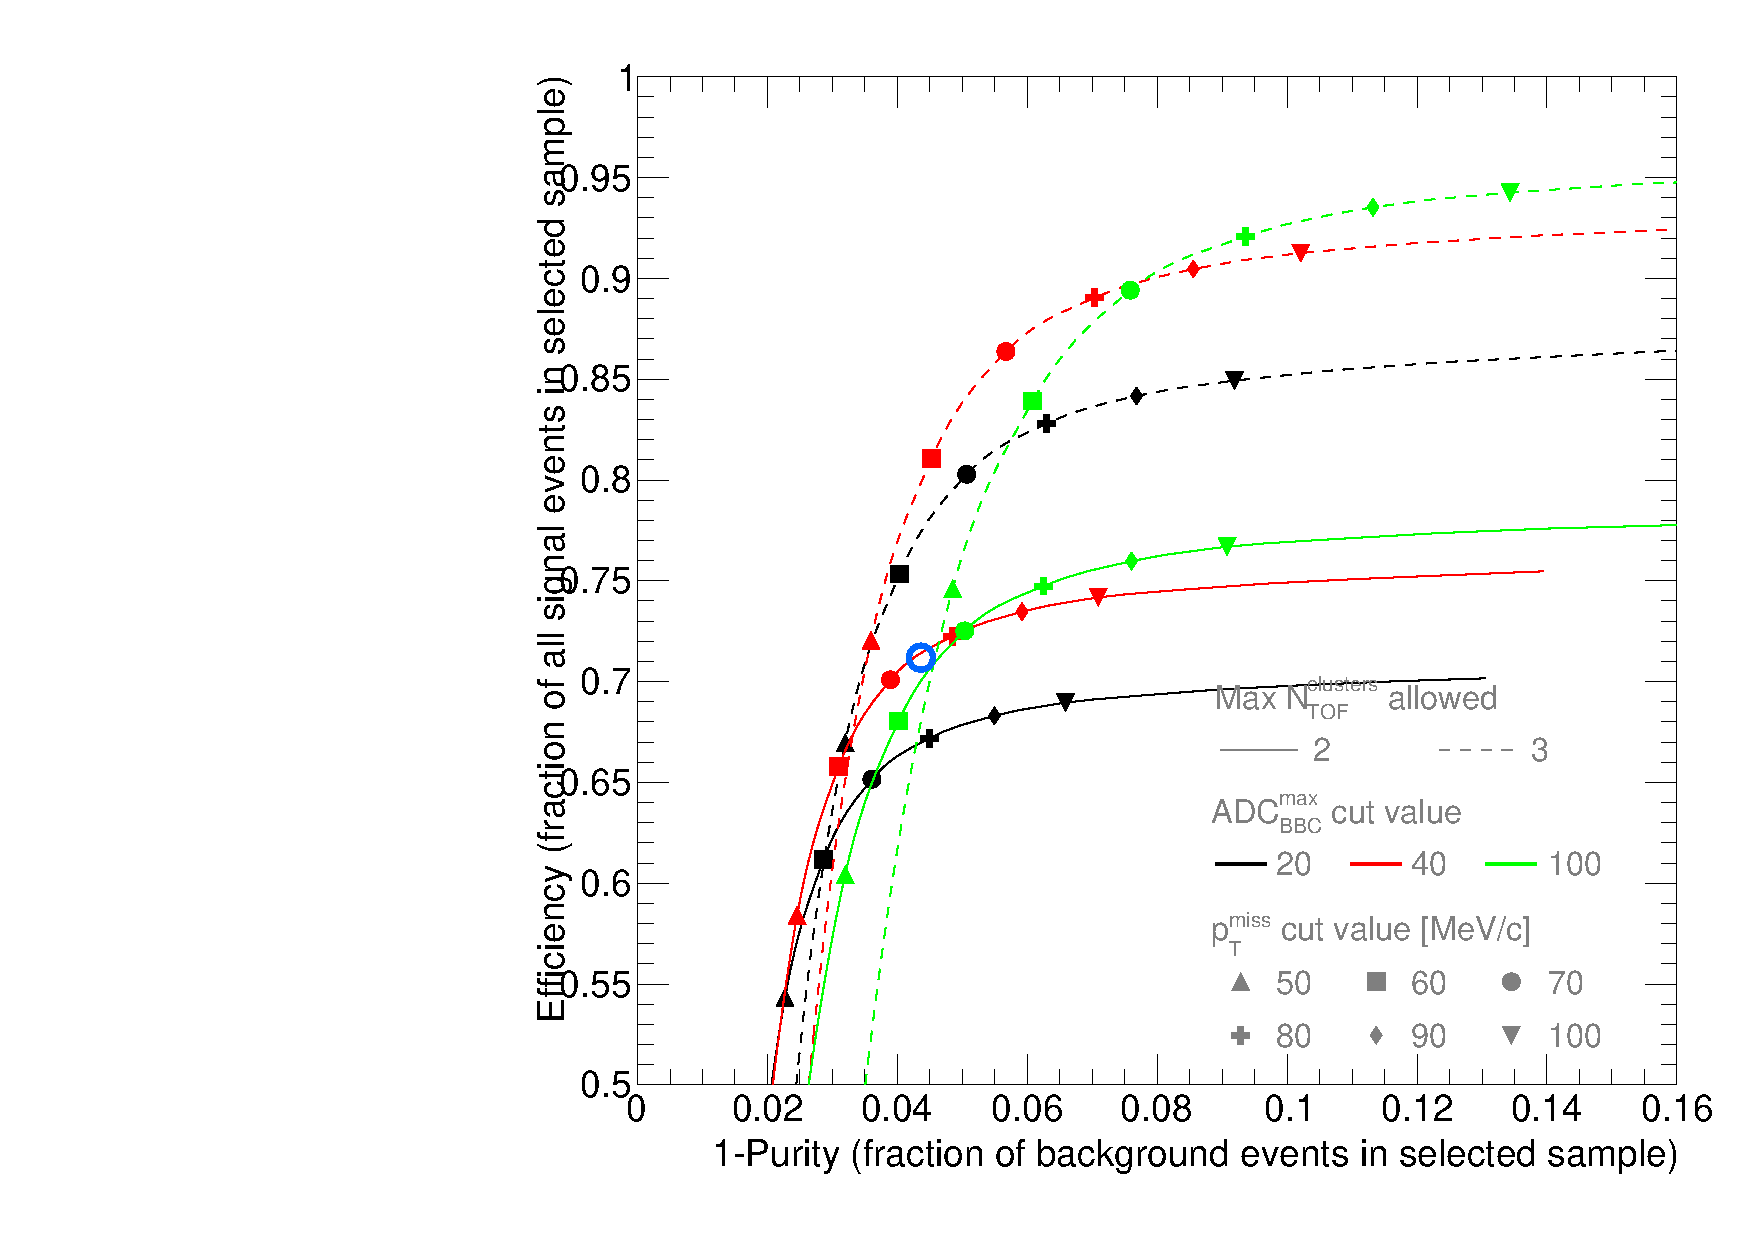
\includegraphics[width=\linewidth]{graphics/eventSelection/ROC_pTmiss.pdf}}
  \end{subfigure}
}%
\quad\quad%
\parbox{0.4725\textwidth}{
  \centering
  \begin{subfigure}[b]{\linewidth}\addtocounter{subfigure}{-2}
                \subcaptionbox{\label{fig:SignificanceVsBkgdFrac}}{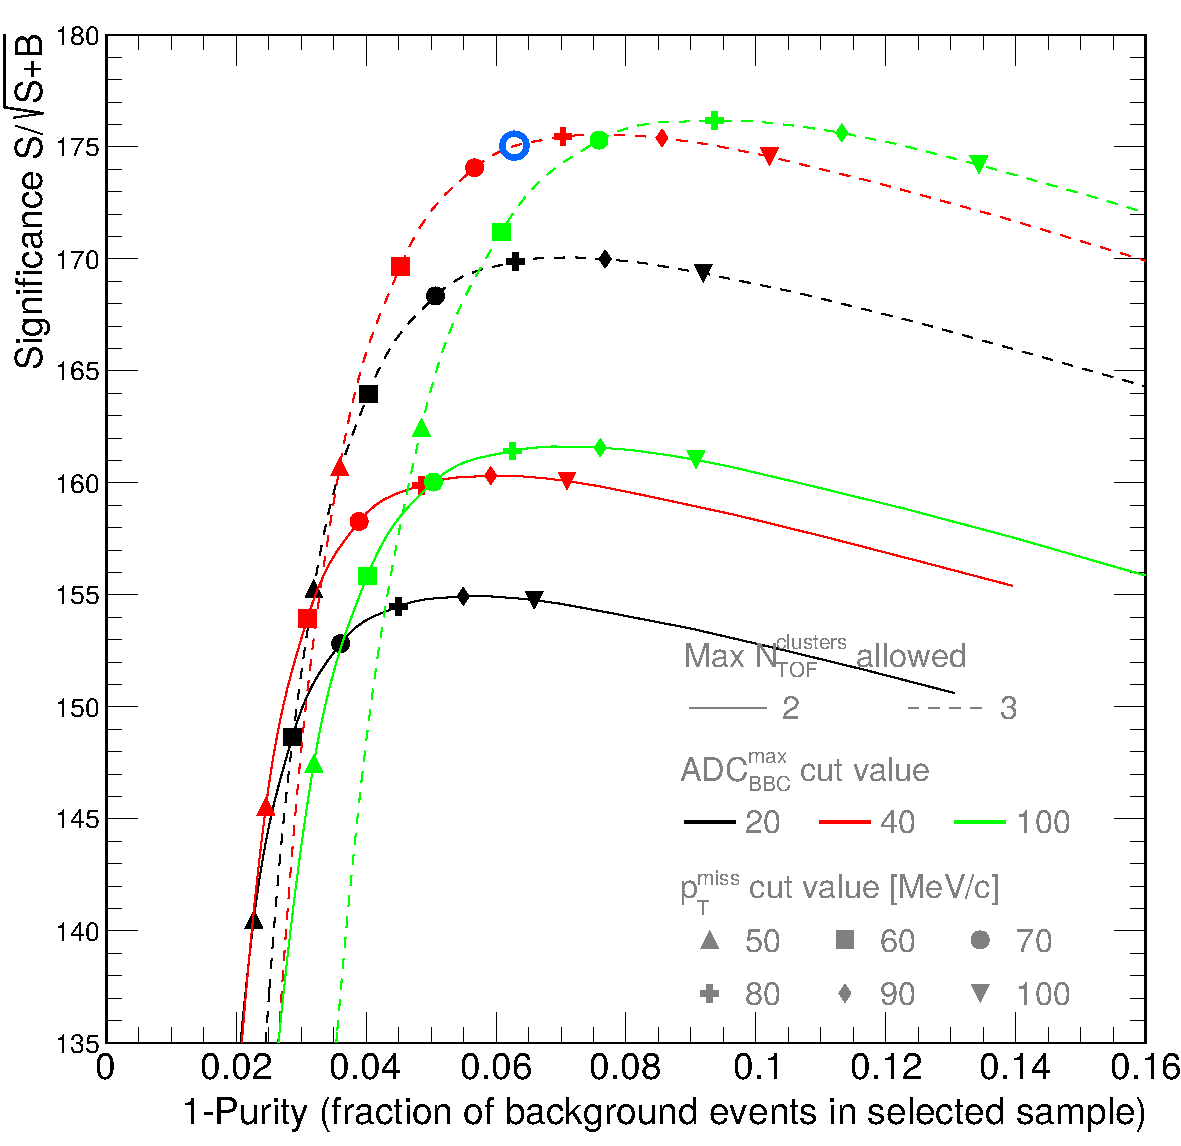
\includegraphics[width=\linewidth]{graphics/eventSelection/BkgdFractionVsEfficiency_pTmiss.pdf}}
  \end{subfigure}\\
  \begin{minipage}[t][1.042\linewidth][t]{\linewidth}\vspace{10pt}
    \caption[Relation between $\pi^{+}\pi^{-}$ significance, efficiency and purity vs. thresholds in cuts~\ref{enum:CutBbcLarge}, \ref{enum:CutTofClusters} and \ref{enum:CutMissingPt}]{Relation between $\pi^{+}\pi^{-}$ signal significance and efficiency (\ref{fig:SignificanceVsEff}), significance and purity (\ref{fig:SignificanceVsBkgdFrac}), and efficiency and purity (\ref{fig:EffVsBkgdFrac}) as a function of cut thresholds in BBC-large veto (\ref{enum:CutBbcLarge}), TOF cluster limit (\ref{enum:CutTofClusters}) and exclusivity cut (\ref{enum:CutMissingPt}). Lines show forementioned relations with changing $p_{T}^\text{miss}$ cut whose some specific values are indicated with different markers. Color denotes ADC threshold in BBC-large veto (black, red or green). Style of line (solid or dashed) denotes $N^{\text{TOF}}_{\text{clstrs}}$ limit. Working point considered optimal is marked with opened blue circle.}\label{fig:workingPoint}
  \end{minipage}
}%

\end{figure}
%---------------------------


\section{Signal per integrated luminosity}

\section{Cut flow}\label{sec:cutFlow}

%---------------------------
\begin{figure}[ht!]
\centering%
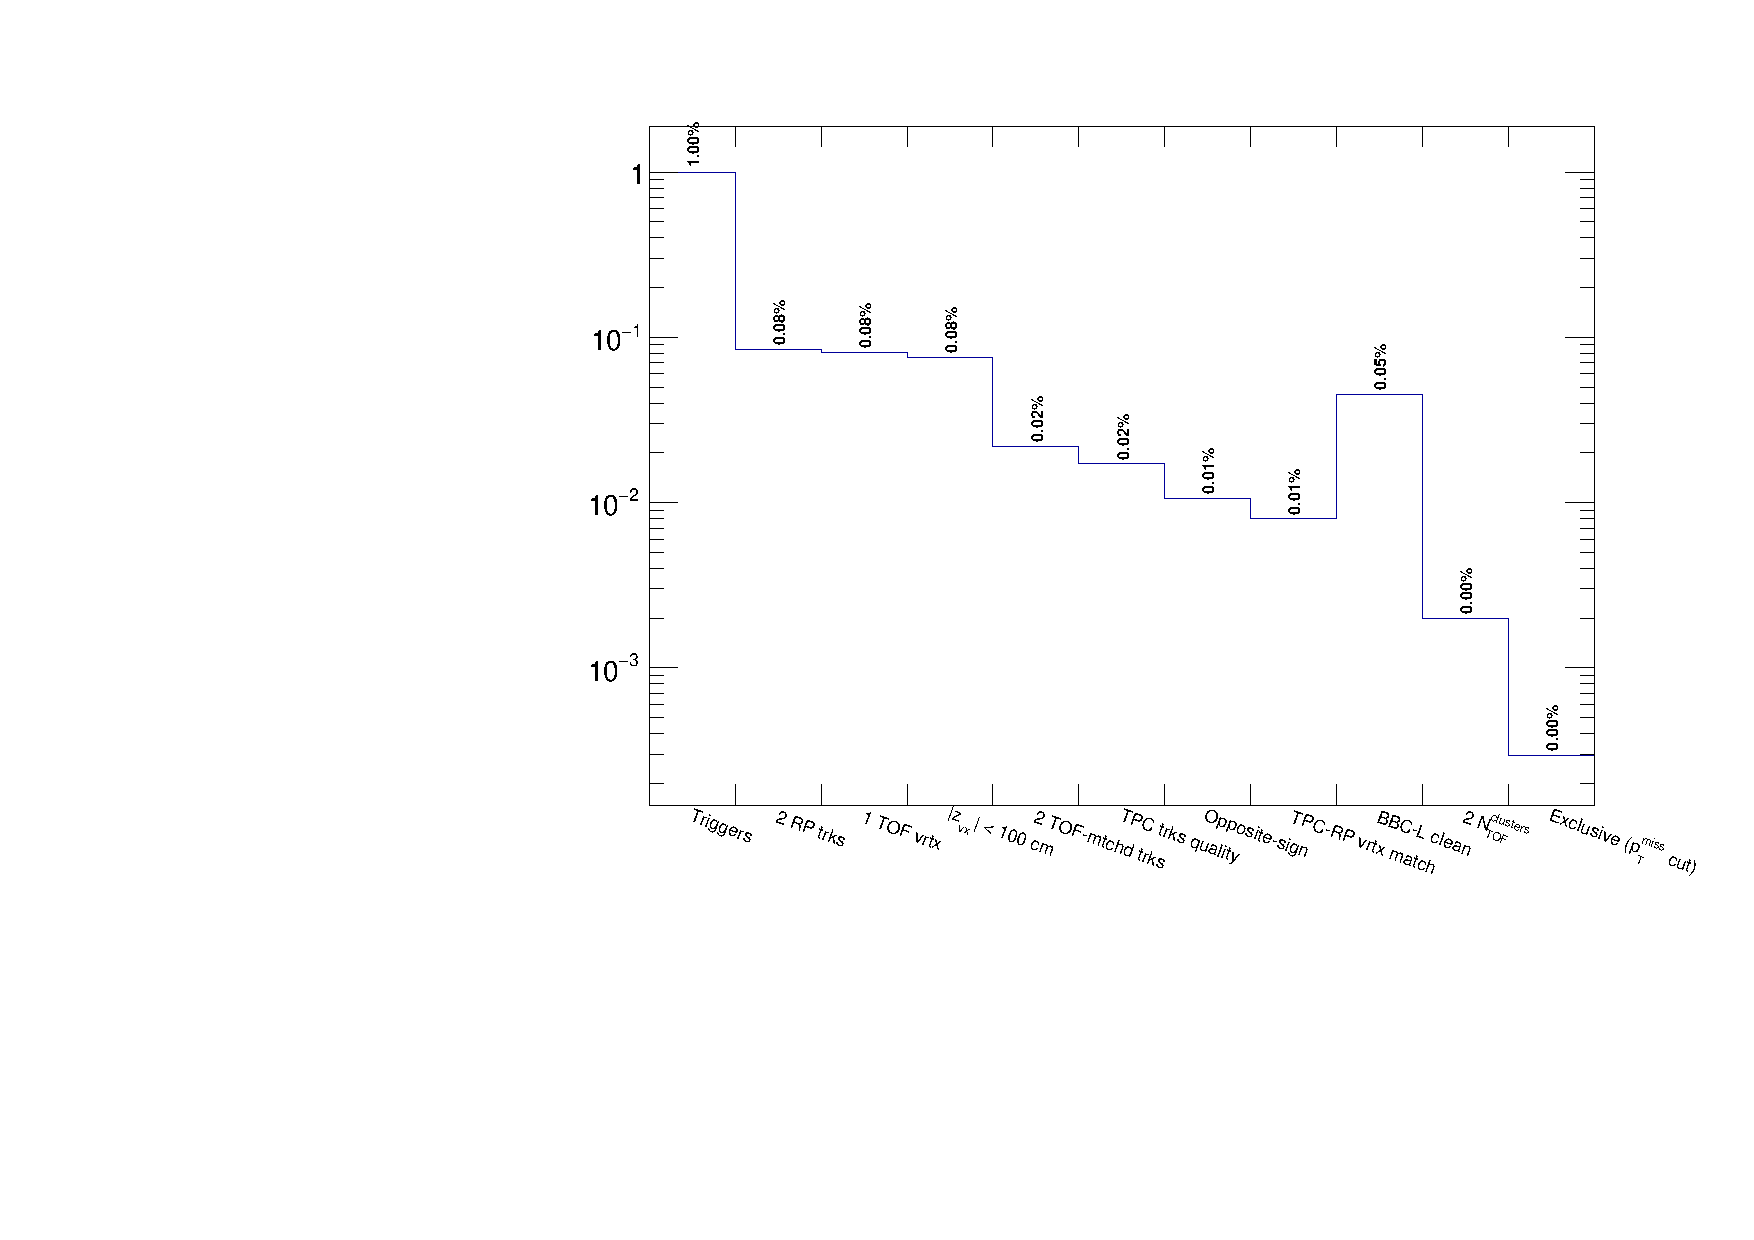
\includegraphics[width=0.85\linewidth,page=1]{graphics/eventSelection/CutFlow.pdf}%
\caption{Cut flow.}\label{fig:CutFlow}%
\end{figure}
%---------------------------
